\documentclass[11pt]{article}
\usepackage{deauthor}
\usepackage{enumitem}
\usepackage{algorithmic}
\usepackage{algorithm}
\usepackage{xcolor}
\usepackage{xspace}
\usepackage{graphicx}
%\usepackage[caption=false]{subfig}
\usepackage{footnote}
\usepackage{hyperref}
\usepackage{multirow}
\usepackage{subfig}
\usepackage{enumitem}
\usepackage{comment}



% simple command to highlight revising
\newcommand\revise[1]{\textcolor{black}{#1}}
% simple command to take notes during drafting process
\newcommand\todo[1]{\textcolor{red}{#1}}
% hybrid index placeholder
\newcommand{\hybridindex}{HQI\xspace}


\begin{document}


\title{Fact Ranking over Large-Scale Knowledge Graphs with Reasoning Embedding Models}

\author{Hongyu Ren$\dagger$\footnote{work done during an internship at Apple.}, Ali Mousavi*, Anil Pacaci*, Shihabur R. Chowdhury*, Jason Mohoney$\ddagger$$^*$, \\ Ihab F. Ilyas*, Yunyao Li*, Theodoros Rekatsinas*\\
  *Apple \\
  $\dagger$Stanford University, hyren@stanford.edu \\
  $\ddagger$University of Wisconsin-Madison, mohoney2@wisc.edu\\
  *{amousavi, apacaci, shihab, iilyas, yunyaoli, thodrek}@apple.com
}


\maketitle
\renewcommand\thesection{\arabic{section}}
\setcounter{section}{0}
\setcounter{figure}{0}
\setcounter{table}{0}

\begin{abstract}
Knowledge graphs (KGs) serve as the backbone of many applications such as recommendation systems and question answering. All these applications require reasoning about the relevance of facts in a KG to downstream applications. In this work, we describe our efforts in building a solution to reason about the importance of facts over continuously updated industry-scale KGs. We focus on the problem of fact ranking and evaluate to what extent modern knowledge graph embedding (KGE) models provide a representation for addressing this problem. To this end, we discuss unique challenges associated with solving this task in industrial settings and evaluate how accurately different KGE models and text-based embedding models can solve the problem of fact ranking.
\end{abstract}
% such as ensuring stability of rankings across updates of a KG


\section{Introduction}\label{sec:ali_intro}

Knowledge graphs (KGs) are the backbone of applications such as question answering in virtual assistants and recommendation systems in. These applications require a broad range of knowledge that is continuously updated with recent facts from disparate data sources~\cite{apple_kp, industry_kgs}. Reasoning about the importance of facts in an industry-scale KG with billions of entities and facts across diverse domains is a challenging problem. An automated and scalable solution scalable across entity types and domains in a KG has obvious benefits.

Here, we focus on the problem of \emph{fact ranking}. Fact ranking provides an importance-based ranking over facts for a given real-world entity. For example, given the question \emph{``What is the occupation of LeBron James?''}, the answer \emph{``basketball player''} should be ranked higher than \emph{``television actor''} or \emph{``screenwriter''} despite the fact that these two are also LeBron James's occupations. Fact ranking generalizes the problem of \emph{recommendation generation}~\cite{bouraga2014knowledge} over KGs. We are interested in facts that cannot be ranked using a simple importance or popularity score. For example, ranking occupation of entities as described earlier. Another example is to generate recommendation for entities that are relevant within users' search context. For example, for the user query \emph{``How tall is LeBron James''}, we want to recommend a ranked list of top KG entities that are related to the query entity ``LeBron James'' and are aligned with users' search intent, \ie, they are ``Person'' entities with a ``height'' attribute. Fact ranking is important during rendering these enriching entity-centric experiences in intelligent assistants. 



In this paper, we propose a solution to fact ranking based on modern Knowledge Graph Embedding (KGE) models and present an experimental evaluation in large-scale settings. Our solution adopts state-of-the-art \emph{multi-hop reasoning} models. Specifically, we build on the recent Query2Box model~\cite{ren2020query2box} and demonstrate how the embeddings obtained by this model can address fact ranking over large-scale KGs. A major challenge in employing KGE models for fact ranking in real-world applications is to reason about the importance score and the rank of a facts obtained by an embedding model. We address this challenge by proposing a new metric for measuring the stability of embedding models across different rounds, namely, an adaptive version of Kendall's Tau that also takes into account the importance scores obtained by the embedding models. In this way, we can better measure the effects of the learned embeddings on the downstream use cases. Our approach is in contrast to using the standard forms of Kendall's Tau or Rank-based Overlap metrics, which measure the consistency across two ranked lists by considering only the number of discordant pairs/swaps between the two lists. We demonstrate that the reasoning-based Query2Box model leads to significantly more stable embeddings compared to one-hop embedding models such as DistMult~\cite{distmult}. We also propose a new indexing scheme and apply multi-query optimization for efficient search over the generated embedding vectors for supporting use-cases such as vector similarity-based related entity search.


Finally, we compare Query2Box against modern generative natural language (NL) models~\cite{liu2019roberta} and demonstrate that NL models require significant fine-tuning of the prompt to obtain similar fact ranking results as the Query2Box model.

\section{Preliminaries}\label{sec:ali_prelim}
We now review background relevant to our study. Our discussion focuses on knowledge graph representation models and aims to highlight the differences between \emph{shallow KG embedding} models such as the popular DistMult~\cite{distmult}, TransE~\cite{transe}, and ~RotatE~\cite{sun2019rotate} models and more recent \emph{reasoning-based embedding models}~\cite{ren2020query2box,ren2020beta}.
\subsection{Shallow Knowledge Graph Embeddings}\label{sec:ali_kg}
A knowledge graph (KG) $\gG=(\gV, \gE, \gR)$ consists of a set of nodes $\gV$, a set of edges $\gE$. $\gG$ also defines a set of relations $\gR$, and each edge $e\in\gE$ represents a triple $(v_s,r,v_o)$ where $r\in\gR$ and $v_s,v_o\in\gV$. Here, $v_s$ corresponds to the vector representation of the \texttt{subject} of the fact that corresponds to the edge and $v_o$ to the \texttt{object} of the fact. Finally, $r$ corresponds to the vector representation of the \texttt{predicate} associated with the triple.

Shallow KG embeddings~\cite{transe,distmult,sun2019rotate,trouillon2016complex} learn an embedding function $f_\theta$ that maps all the entities and relations on the graph to latent space in order to preserve the structure of graph. Most KG embeddings implement the embedding function $f_\theta$ as a matrix lookup. Specifically, the parameters include an entity embedding matrix $\rmV_\theta\in\R^{|\gV|\times d}$ and a relation embedding matrix $\rmR_\theta\in\R^{|\gR|\times d}$, where $d$ is the latent space dimension. 

\newparagraph{Training Shallow KG Embeddings:}
In order to train the two embedding matrices, these methods optimize a contrastive objective, which is to minimize a predefined distance function \texttt{Dist} of existing edges $e=(v_s,r,v_o)\in\gE$ while maximize that of non-existing edges $e'=(v_s,r,v_o')\notin\gE$. Different shallow KG embeddings have different definitions of the distance function \texttt{Dist}, the detail is listed in Table \ref{tab:kg-model}. 
In previous KG embedding works~\cite{sun2019rotate,zhang2019quaternion}, the loss function in the contrastive objective is defined as:
\begin{align} 
    \gL &= -\log \sigma \left(\gamma - \distt{v_s}{r}{v_o} \right) 
    - \sum_{j=1}^k \frac{1}{k} \log \sigma \left(\distt{v_s}{r}{v_{o_j}'} -\gamma \right),\label{eq:kgelossfunc}
\end{align}
where $\sigma$ is the sigmoid function, $\gamma$ is the margin. 
We optimize over the loss function using stochastic training for several iterations. In each iteration, these methods sample a batch of existing edges from the graph and construct non-existing edges by keeping the subject $v_s$ and the type of the edge $r$ fixed while perturbing the object $v_o$.


\begin{table}[t]
\small
\centering
\caption{The distance function of shallow KG embeddings and KG reasoning embeddings. 
\label{tab:kg-model}}
\resizebox{0.9\columnwidth}{!}{%
\begin{tabular}{ccc}
	\toprule
Model & Embedding Space & Distance \\
\hline
TransE~\cite{transe} & $\Em{v_s},\Em{v_o}\in\RR^d$, $\Em{r}\in\RR^d$ & $\|\Em{v_s}+\Em{r}-\Em{v_o}\|$ \\
\hline
RotatE~\cite{sun2019rotate} & $\Em{v_s},\Em{v_o}\in\CC^d$,$\Em{r}\in\CC^{d}$ & $\|\Em{v_s}\circ\Em{r}-\Em{v_o}\|$ \\\hline
DistMult~\cite{distmult} & $\Em{v_s},\Em{v_o}\in\RR^d$,$\Em{r}\in\RR^{d}$ & $-<\Em{v_s},\Em{r},\Em{v_o}>$ \\\hline
ComplEx~\cite{trouillon2016complex} & $\Em{v_s},\Em{v_o}\in\CC^{d}$, $\Em{r}\in\CC^{d}$ & $-\text{Re}(<\Em{v_s},\Em{r},\overline{\Em{v_o}}>)$ \\\hline
Q2B~\cite{ren2020query2box} & $\Em{v_s},\Em{v_o}\in\RR^{d}$, $\Em{r}\in\RR^{2d}$ & $\texttt{Dist}_\text{out}+\alpha\texttt{Dist}_\text{in}$ \\
% BetaE~\cite{ren2020beta} & $\Em{v_s},\Em{v_o}\in\RR^{d}$, $\Em{r}\in\RR^{d}$ & $\texttt{KL}(\text{Beta}(\Em{v_o});\text{Beta}(\texttt{MLP}(\Em{v_s},\Em{r})))$ \\

	\bottomrule
\end{tabular}
}%
\end{table}
\subsection{KG Reasoning Embeddings}\label{sec:ali_background}
KG reasoning embedding methods generalize the shallow KG embeddings to more complex reasoning tasks. KG reasoning embeddings also consider multi-hop reasoning over the KG, \ie, answering complex logical queries with logical/set operators including conjunction, disjunction and negation, \eg, \qu{Predict drugs that might target proteins that are associated with a given disease, and do not have a given side effect}~\cite{hamilton2018embedding}. 
In order to answer such complex queries, one may need to perform multiple reasoning steps and graph traversal -- first find all the proteins associated with the disease, and predict drugs $\gD_1 \subset \gV$ that bind with the proteins, at the same time find the drugs $\gD_2 \subset \gV$ that have the side effect and take complement of the set $\overline{\gD_2}$, and finally take the intersection of the two sets $\gD_1\cap\overline{\gD_2}$ to achieve the answers to the query. 
One of the main challenges of the above graph traversal method is that it suffers from missing and noisy information on the graph.
The key insight of KG reasoning embedding methods is to embed these complex queries in the same latent space as the entity embeddings so that all the reasoning steps can be done in the embedding space instead of symbolic graph traversal. 
In detail, we follow the logical queries defined in \citet{ren2020beta}. 
\begin{definition}[First-order logic queries]\label{def:query}
A first-order logic query $q$ consists of a non-variable anchor entity set $\gV_q \subseteq \gV$, existentially quantified bound variables $V_1, \dots, V_k$ and a single target variable $V_?$, which provides the query answer. The disjunctive normal form of a logical query $q$ is a disjunction of one or more conjunctions. 
\begin{align*}
\centering
    q[V_{?}] = V_?\:.\:\exists V_1, \ldots, V_k : c_1 \vee c_2 \vee ... \vee c_n
\end{align*}
\begin{enumerate}
    \item Each $c$ represents a conjunctive query with one or more literals $e$. $c_i = e_{i1} \wedge e_{i2} \wedge \dots \wedge e_{im}$.
    \item $e$ represents an atomic formula or its negation. $e_{ij} = r(v_a, V)$ or $\neg\:r(v_a, V)$ or $r(V', V)$ or $\neg\:r(V', V)$, where $v_a \in \gV_q$, $V \in \{V_?,V_1,\ldots,V_k\}$, $V' \in \{V_1,\ldots,V_k\}$, $V\neq V'$, $r \in \gR$.
\end{enumerate}
\end{definition}

% We can derive a computation graph for each query in Def.~\ref{def:query}. This computation graph represents the reasoning process in order to answer the query. Specifically, we can take each atomic formula $r(V_1, V_2)$ of the query and represent this formula with a graph with two nodes $V_1$ and $V_2$, and a directed edge $r$ that connects the two nodes. We merge the graphs of all atomic formula with logical edges including conjunction (set intersection), disjunction (set union) and negation (set complement). The merged graph will be the computation graph for this query. Each node of the computation graph represents a set of entities in the KG and each edge represents a logical/relational transformation of this set. 
% The computation graphs of FOL queries are heterogeneous \emph{trees}, where each leaf node corresponds to a set of cardinality one that contains a single anchor entity $v_a\in\gV_q$ (note that one anchor entity may appear in multiple leaf nodes) and the root node represents the unique target variable, which is the set of answer entities. 
% Each edge of the computation graph can take the following operations:
In order to reason over and embed such queries, one needs to consider the following operations. KG reasoning methods design neural logical operators that simulate their real counterparts. We refer the readers to \citep{ren2020query2box} for more details.
\begin{enumerate}
    \item \textbf{Relation Projection:} Given a set of entities $S \subseteq \gV$ and relation type $r \in \gR$, compute adjacent entities $\cup_{v \in S} A_r(v)$ related to $S$ via $r$: $A_r(v) \equiv \{v^{\prime} \in \gV: \ (v, r, v^{\prime})\in\gE\}$.
    \item \textbf{Intersection:} Given sets of entities $\{ S_1, S_2, \ldots, S_n\}$, compute their intersection $\cap_{i = 1}^n S_i$.
    \item \textbf{Complement/Negation:} Given a set of entities $S \subseteq \gV$, compute its complement $\overline{S} \equiv \gV \:\backslash\: S$.
    \item \textbf{Union:} Given sets of entities $\{ S_1, S_2, \ldots, S_n\}$, compute their union $\cup_{i = 1}^n S_i$.
\end{enumerate}


% To answer a given query, we can follow the query formula and execute logical operators. We denote the answer set as $\gA_q^\gG$, which represents the set of entities on $\gG$ that satisfy $q$, \textit{i.e.}, $v \in \gA_q^\gG \iff q[v]=\texttt{True}$. Note that this symbolic traversal of the computation graph is equivalent to traversing the KG, however, it has exponential computation complexity with respect to the number of hops and also cannot handle noisy or missing edges in the KG.

\newparagraph{Capturing Relational Context:} While KG reasoning queries have been traditionally proposed to answer complex queries in the presence of incomplete KGs, here, we utilize them to learn vector representations of the entities that are not biased towards one-hop relationships but take into account a richer \emph{relational context}. We use a set of \emph{query templates} (see Figure~\ref{fig:query}) to \emph{generate a sample workload of queries that can be answered over the input KG} and use that payload to learn robust entity representations as we discuss next. \emph{We experimentally show (see Section~\ref{sec:ali_experiment}) that this relational bias in the training process leads to entity representations that are more robust and lead to more stable representations (see Section~\ref{sec:ali_experiment}).}

\begin{figure}
        \centering
      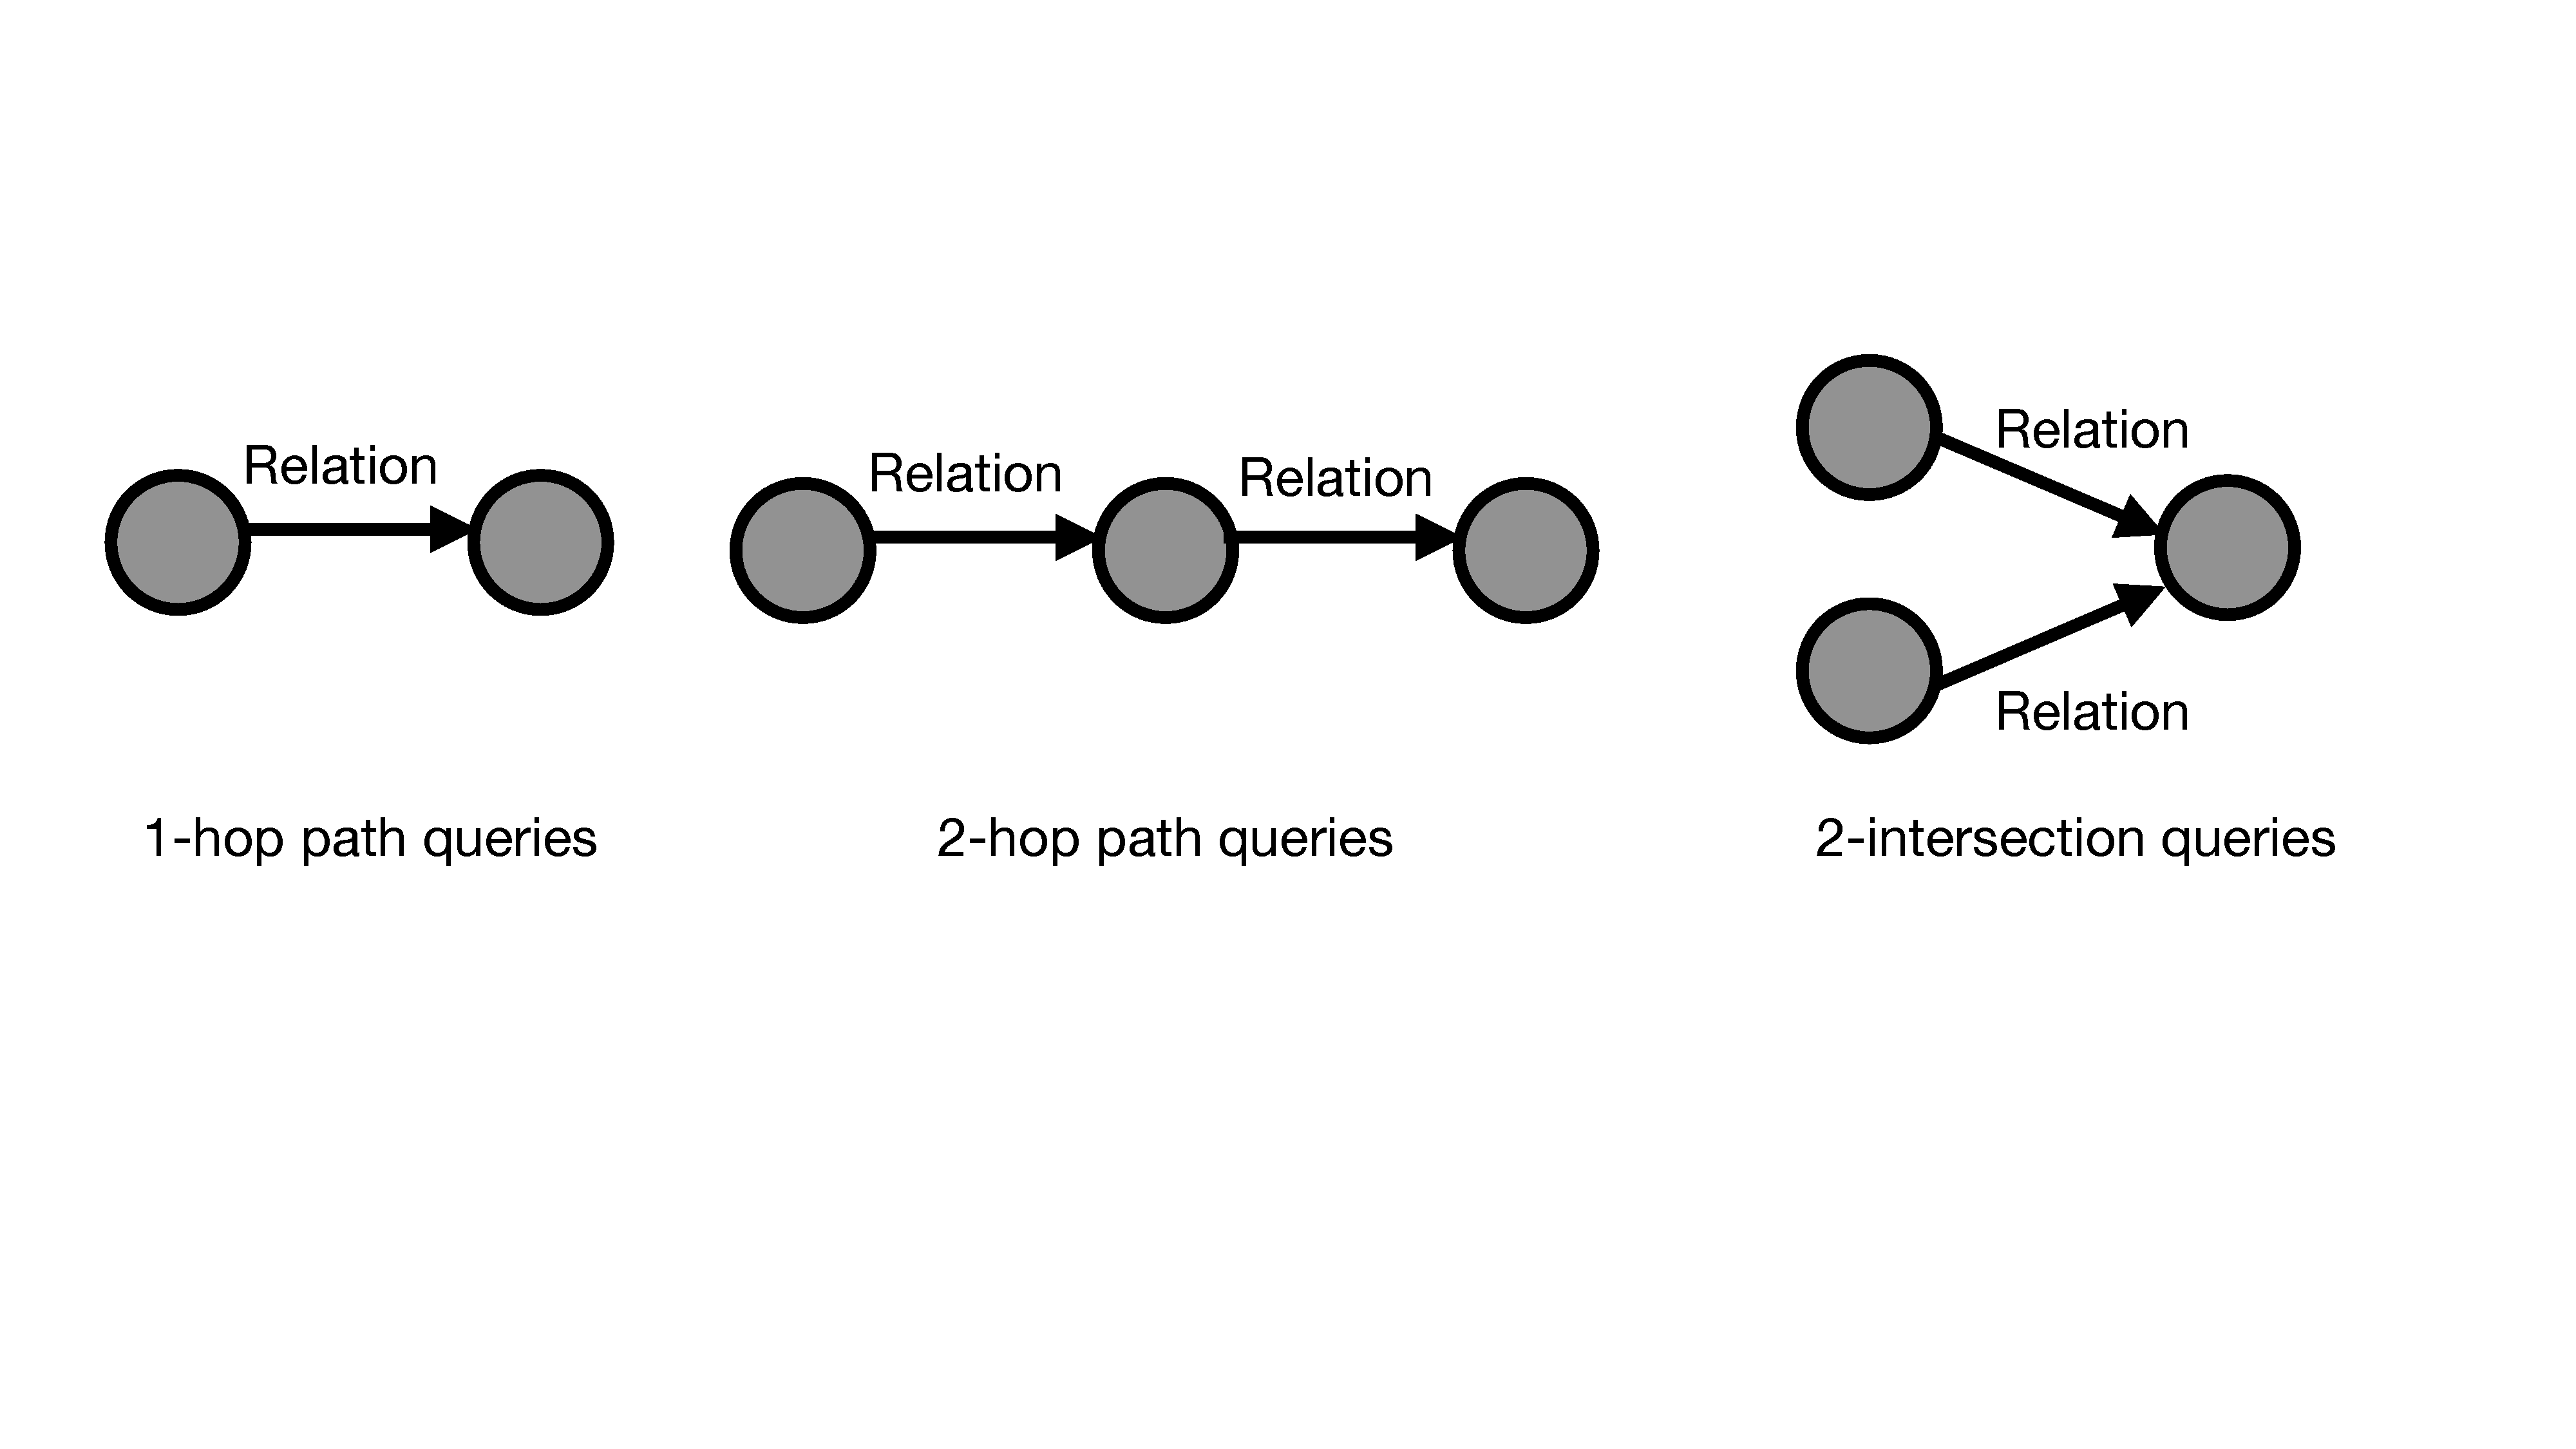
\includegraphics[width=0.5\columnwidth]{submissions/Ali2023/figures/query.pdf}
      \caption{Types of queries we consider to train Query2box.}
    \label{fig:query}
\end{figure}

\newparagraph{Training KG Reasoning Embeddings:} For a KG, $\gG = (\gV, \gE, \gR)$, and a query $q$, we need to learn an embedding function $f_\theta$ that maps from a computation graph of a query to its embedding with the parameterized neural logical operators. Together with the entity and relation embedding matrices (same as the shallow KG embeddings), $f_\theta$ also embeds all the nodes on the graph by embedding lookup. In order to measure the similarity/distance between a query $q$ and an entity $v \in \gV$, a distance function $\texttt{Dist}(\cdot,\cdot)$ is defined that takes as input the query embedding $f_\theta(q)$ and the entity embedding $f_\theta(v)$ and outputs the distance. The distance function $\texttt{Dist}(\cdot,\cdot)$ is tailored to different embedding space and model design $f_\theta$ as in Table \ref{tab:kg-model}.

During training, we are given a data sampler $\gD$, each sample in $\gD$ is a tuple $(q,\gA_q,\gN_q)$, which represents a query $q$, its answers $\gA_q\subseteq \gV$ and the negative samples $\gN_q\subseteq\overline{\gA_q}$. The training objective is to minimize the distance between the query embedding and its answers $\texttt{Dist}(q, v), v\in\gA_q$ while maximizing the distance between the query embedding and the negative samples $\texttt{Dist}(q, v'), v'\in\gN_q$, optimizing a contrastive loss term similar to the shallow KG embeddings. As used in most previous KG reasoning embedding works~\cite{ren2020beta,ren2020query2box}, the loss is defined as:
\begin{align} 
    \gL &= -\log \sigma \left(\gamma - \texttt{Dist}(q,v) \right) 
    - \sum_{j=1}^k \frac{1}{k} \log \sigma \left(\texttt{Dist}(q,v_j^{\prime})-\gamma \right),\label{eq:lossfunc}
\end{align}
where $\gamma$ is a margin hyperparameter and $\sigma$ is the sigmoid function. 

\section{Fact Ranking}\label{sec:usecase}

\revise{Here we introduce the task of fact ranking and its corresponding applications that power critical user experiences over KGs.
We define a fact on KG as a triple $(v_s, r, v_o)$, where $v_s$ and $v_o$ are entities and $r$ is a relation type from the KG.
User queries we target (such as the  \emph{``What is the occupation of LeBron James?''}) correspond to queries of the form $q=(v_s, r, ?)$ .
}

% We now introduce the tasks of fact ranking that is a critical production task over KGs. First we define a fact on KG as a triple $(v_s, r, v_o)$, where $v_s$ and $v_o$ are entities and $r$ is a relation type from the KG. These tasks correspond to queries of the form $q=(v_s, r, ?)$.



\subsection{Problem Description}\label{sec:ranking}
Intelligent assistants rely on entity-centric experiences to answer user queries. For many of these experiences, facts or answers to queries are of different importance/accuracy/uncertainty to users. Besides providing all the answers, one key aspect of service quality is to display relevant facts in a sorted way according to the importance or uncertainty score. For example, the answer to a query \qu{What is the occupation of Selena Gomez?} includes \emph{singer} and \emph{child actor}, but for the majority of users, we know the answer \emph{singer} should rank higher than \emph{child actor}.
The goal of fact ranking is to rank all the answers to a given set of queries that aligns well with user expectation. Fact ranking is ubiquitous in intelligent assistants and the key to improving the user experience. 

We define fact ranking as follows: Given a query $q=(v_s, r, ?)$ for a subject $v_s$ and a predicate $r$ we see to find answers $\gA_q$ (achieved by graph traversal as discussed in \Secref{sec:prelim}) for the missing object. The goal of fact ranking is to find a function $\rank{a}$ which can be used to obtain an importance ranking for each answer $a\in\gA_q$ and generate the ranking list $[\rank{a_1}, \dots, \rank{a_n}], \:\: a_1, \dots, a_n\in\gA_q$. We focus on queries that target facts that cannot be ranked using simple popularity scores, \eg, occupations, genres \etc, (an occupation is not necessarily more important than the other).

Unsupervised machine learning (ML) mechanisms are needed to learn a function $\rank{\cdot}$. It is typical that KGs do not associate any importance scores and weights to their edges, which applies to many large KGs including FreeBase~\cite{bollacker2008freebase} and WikiData~\cite{wikidata}. Consequently, it is not possible to use simple traversal mechanisms to implement the ranking functions for fact ranking and different mechanisms need to be considered. Such a mechanism may correspond to PageRank-based algorithms which can be used to assign an importance score for each answer $a$ (or fact $(q,a)$ with personalized PageRank), however, they are often not effective on such large-scale heterogeneous graphs where multiple edge types exist~\cite{10.1145/3447548.3467342}. To alleviate these challenges, we consider a setting (see Section~\ref{sec:method}) where \emph{unsupervised representation learning} is used to learn Function $\rank{\cdot}$.

\iffalse
\subsection{Fact Verification}\label{sec:verification}
As introduced in \Secref{sec:intro}, industrial KGs are often noisy and contain missing facts. A critical task is to verify facts and impute missing facts to deliver high-accuracy services to users. 
Most previous KG works formulate and evaluate this problem as a \emph{link prediction task}~\cite{wang2017know}: Given a query $q=(v_s, r, ?)$ and its missing object $v_o$, the methods plug in all the entities on the KG $\forall v\in\gV$ as object, score them and rank the missing objects against other entities. The goal is that the missing objects rank higher than the other true negative object entities. Based on the ranking, different methods are evaluated using different functions of the ranking, \eg, mean reciprocal rank (MRR), Hits@$k$ (H@$k$), for those missing answers/facts. 
% 
However, this formulation is impractical in real use cases since different queries vary in the number of answers and it is hard to define a threshold that strikes a good balance between covering all promising facts to verify and at the same time keep the size of the set minimum to reduce the cost of human curation.
% 

In this work, we define the fact verification task as follows:
Given a set of triplets $\{(v_s^1, r^1, v_o^1), \dots, (v_s^n, r^n, v_o^n)\}$ to verify, the goal is to prioritize and select the most promising ones and use human curators to manually check the prioritized facts. Adopting a human-in-the-loop approach ensures that the strict precision requirements for industrial KGs are satisfied~\cite{apple_kp}. Promising triplets can either be (1) existing triplets on the graph that are considered as \emph{False}, and thus, human curators are required to check and remove the triplets from the graph or (2) non-existing triplets on the graph that are missing but are correct with high probability.
The task definition shares a similar flavor with the triplet classification task. The idea is to perform a binary classification task over the list of triplets and find the promising ones.
In this task, we evaluate methods using the AUC-ROC score, which measures how much better the method is compared with random sampling triplets from the given list.
\fi


\subsection{A Solution with KG Embeddings}\label{sec:method}
We obtain a solution to the fact ranking problem by leveraging graph embedding models. This solution applies to both shallow KG embeddings and KG reasoning embeddings. 
The idea is to first train the entity embeddings, relation embeddings, and neural logical operators on the KG using standard training protocols \cite{distmult,ren2020query2box} (see \Secref{sec:background}). Then, given a fact $(v_s,r,v_o)$, we can use the pre-trained embeddings to efficiently calculate the distance $\distt{v_s}{r}{v_o}$. The distance plays a crucial role for solving the fact ranking problem since it represents a \emph{proxy of plausibility of a fact}. This solution is inspired by our prior work on error detection, missing value imputation, and data repairs which showed that all problems correspond to inference tasks over a pre-trained model that learns how to \emph{reconstruct} the input data~\cite{de2018formal}. Nonetheless, using the distance obtained by different KG embedding models raises two critical considerations for industrial settings. 

For fact ranking, the distance obtained by the KG embedding model can be applied to rank the candidate objects for a specific subject and object configuration. However, different models can learn significantly different geometries and in most cases the distances in these spaces can lead to significant variations in the obtained rankings. In the settings we consider, it is critical that the rankings obtained are stable (i.e., we do not have significant variations in the order of different objects) across training iterations of the embedding model. To this end, we use a post-processing step that verifies the stability of KG embedding models before deployment. This post-processing step utilizes a consistency metric that extends standard ranking comparison methods such as Kendall's Tau to also consider the distance value associated with each query (see Section~\ref{sec:consistency}). 

%For fact verification, we convert the distances into \emph{calibrated confidence scores} across different subjects/predicates in the KG. This step is important as we need to obtain a unified prioritization score to decide which facts should be surfaced for verification to human graders. Past works~\cite{DBLP:conf/iclr/TabacofC20, sun2019re} have shown that the absolute distance calculated using \eqref{eq:kgelossfunc} is not well calibrated and leads to biased results. To this end, we design a separate post-processing step that converts the raw distance measurements from KG embeddings to calibrated scores. We provide a detailed discussion in Section~\ref{sec:calibration}.


% \section{A KGE Framework}\label{sec:method}
% We propose a framework that uses graph embedding models to obtain a unified solution for fact ranking and fact verification. Our solution extends to both shallow KG embeddings as well as the KG reasoning embeddings. 
% The idea is to first train the entity embeddings, relation embeddings, and neural logical operators on the KG using standard training protocols \cite{yang2014embedding,ren2020query2box} as introduced in \Secref{sec:background}. Then given a fact $(v_s,r,v_o)$, we can use the pre-trained embeddings to efficiently calculate the distance $\texttt{Dist}(f_\theta(v_s), f_\theta(r), f_\theta(v_o))$. The distance plays a crucial role in our framework to solve both tasks since it represents our belief over the plausibility of a fact. 
% \todo{Revisit: As an overview, for fact ranking, our framework ranks all the answers of a query using the distance score. To satisfy the two requirements, we conduct a user study on several facts to measure the utility of our framework on the ranking task and design various metrics to measure the consistency of the ranking lists of various facts across multiple runs of training. 
% For fact verification, we develop a novel method based on in-distribution detection and out-of-distribution detection in order to calibrate the distance across facts and thus prioritize those most promising facts for human curators to verify.}

\section{Consistency in Fact Ranking}\label{sec:consistency}
We consider different ways to measure the stability of ranking across different training runs. Given a query $(v_s, r, ?)$ and its answers $\gA_q=\{a_1, \dots, a_n\}$, we calculate: $d_i = \distt{v_s}{r}{a_i},$ $\forall i=1, \dots, n,$
and create a distance list $\texttt{DistList}=[d_1, \dots, d_n], d_i\in\R$ and a ranking list of the answers by the distance $\texttt{RankList}=[\rank{a_1}, \dots,  \rank{a_n}], \rank{a_i}\in\{1, 2, \dots, n\}$. We consider training KG embeddings multiple times, and obtain multiple $\texttt{DistList}$ and  $\texttt{RankList}$. Our goal is to measure the stability/consistency of the lists across different runs. We assume the KG stays unchanged across different runs/training of the embedding models, hence the items in the list of a query also remain the same. 

To measure the stability of ranking, \ie, compare whether two $\texttt{RankList}$ from two runs are consistent, we consider several metrics, including 1) the Kendall rank correlation coefficient, 2) a weighted version of Kendall's Tau, 3) set-based overlap, and 4) rank-biased overlap. Given two distance lists $\texttt{DistList}_1=[x_1, \dots, x_n]$ and $\texttt{DistList}_2=[y_1, \dots, y_n]$, the four metrics are calculated as:
\begin{enumerate}
    \item Kendall's Tau: $\frac{m_c - m_d}{\binom{m}{2}}$, where $m_c$ is the number of concordant pairs between $\texttt{DistList}_1$ and $\texttt{DistList}_2$, and $m_d$ is the number of discordant pairs. A pair of $(i, j)$ is concordant if the sort order of $(x_i, x_j)$ and $(y_i, y_j)$ is the same, otherwise the pair is discordant. Kendall's Tau ranges from -1 to 1.
    \item Weighted Tau: It is an extension of Kendall's Tau where each pair also has a weight that is inverse-proportional to the rank, \ie, low ranking objects are not as important as the top ranking objects.
    \item Rank-biased overlap (RBO): $(1-p)\sum_{i=1}^n p^{i-1} \cdot A_i$, where $i$ is the depth of the ranking being examined. With $ArgSort$ function, let $\texttt{ASList}=ArgSort(\texttt{DistList})$, we define $A_i=\frac{|\texttt{ASList}_1[:i]\cap\texttt{ASList}_2[:i]|}{i}$. The idea of RBO is to compare the overlap of the two rankings at incrementally increasing depths. It is a weighted metric, which means that the top rank items get higher weights. 
\end{enumerate}

% \todo{residue function, computation graph, improve figure, unify title capital}
However, the downside of the above metrics is that they do not explicitly consider the absolute value of items in \texttt{DistList}. One observation is that when two answers have similar distance with the query embedding, a swap in the ranking of the two answers from two runs should not matter as much as a swap in the ranking when the two answers have different distance to the query embedding. Consider the following two scenarios, assume in both scenarios, the length of the \texttt{DistList} is 3. In Scenario \#1 we have $\texttt{DistList}_1: [0.20, 0.30, 0.33] \quad \texttt{DistList}_2: [0.45, 0.61, 0.60]$ and in Scenario \#2 we have $\texttt{DistList}_1: [0.20, 0.30, 0.63] \quad \texttt{DistList}_2: [0.45, 0.61, 0.50]$.
% \begin{align*}
% \text{Scneario \#1:}& \\
% \texttt{DistList}_1&: [0.20, 0.30, 0.33] \quad \texttt{DistList}_2: [0.45, 0.61, 0.60] \\
% \text{Scneario \#2:}& \\
% \texttt{DistList}_1&: [0.20, 0.30, 0.63] \quad \texttt{DistList}_2: [0.45, 0.61, 0.50]
% \end{align*}

Although in both scenarios, there exists one discordant pair (the second and third item), yet in Scenario \#1, the two items have extremely close distance compared with Scenario \#2. So an ideal metric would output a higher consistency score for Scenario \#1 than Scenario \#2. However, all above metrics give the same results.


\begin{algorithm}[t]
\small
\caption{AdaptiveCluster}
\label{alg:adaptive-cluster}
\SetKwInOut{Input}{Input}
\SetKwInOut{Output}{Output}
\Input{A list of distance of answers $\texttt{DistList}=[x_1, \dots, x_n]$, a scalar threshold $\delta'$ (hyperparameter).}
\Output{A list of cluster IDs $\texttt{ClusterList}$.}
\BlankLine
$\texttt{DiffList} = []$\;
\For{$i\gets 1$ \KwTo $n$}{
    $\texttt{DiffList}.\text{append}(x_i - x_{i-1})$\;
}
$\mu=\texttt{DiffList}.\text{mean}()$, $\sigma=\texttt{DiffList}.\text{std}()$\;
Threshold $\delta=\min(\mu-0.2\sigma,\: \delta')$\;
$\texttt{ClusterList}=[0]$, $clusterid=0$\;
\For{$i\gets 0$ \KwTo $n-1$}{
    \If{$\texttt{DiffList}[i]>\delta$}{
        $clusterid++$\;
    }
    $\texttt{ClusterList}.\text{append}(clusterid)$\;
}
\Return{\texttt{ClusterList}}\;
\end{algorithm}

\begin{algorithm}[t]
\small
\caption{Adaptive Tau}
\label{alg:adaptive-tau}
\SetKwInOut{Input}{Input}
\SetKwInOut{Output}{Output}
\Input{Two lists of distance of answers $\texttt{DistList}_1$, $\texttt{DistList}_2$, a scalar threshold $\delta'$ (hyperparameter).}
\Output{Kendall's Tau coefficient.}
\BlankLine
$\texttt{ClusterList}_1=\text{AdaptiveCluster}(\texttt{DistList}_1, \delta')$\;
$\texttt{ClusterList}_2=\text{AdaptiveCluster}(\texttt{DistList}_2, \delta')$\;
\Return{KendallTau($\texttt{ClusterList}_1$, $\texttt{ClusterList}_2$)}\;
\end{algorithm}

To address the above shortcoming, we use an evaluation metric that adaptively considers the margins of different items when measuring the consistency of two \texttt{DistList}. In order to identify the items with close values, we sort the \texttt{DistList}, calculate the difference between neighbor items, and measure the average and variance, which we use to set as a threshold. Then, we loop over all the items and aim to cluster the item by checking whether the difference between the current item and the previous item is larger than the threshold. 
For items in the same cluster, we assign the same value to them such that they will have the same ranking. Finally, we run Kendall's Tau metric over this updated list. The details are shown in Algorithms \ref{alg:adaptive-cluster} and \ref{alg:adaptive-tau}.
We refer to this method as \emph{Adaptive Tau} since it considers the absolute value of the discordant pairs using clustering with an adaptive threshold. An experimental analysis of the different metrics is shown in Section~\ref{sec:experiment}. We find that Adaptive Tau provides a more precise description of the stability and utility of the rankings obtained by embedding models.

%%%%%%%%%%%%%%%%%%%%%%%%%%%%%%%%%%%%%%%%%%%%%%%%%%%%%%%%%%%%%%%%%%%%%%%%%%%%%
\iffalse

\section{Calibrated Fact Verification}\label{sec:calibration}
Given a set of facts $\gE_\text{V}=\{(v_s^1, r^1, v_o^1), \dots, (v_s^n, r^n, v_o^n)\}$, the goal of fact verification is to prioritize a subset $\gE_\text{P}\subseteq \gE_\text{V}$ that are likely to have the opposite label, which we refer to as the \emph{promising triples}.
This subset includes both existing facts in the KG that may be False, or non-existing triplet facts that may be True.
  
Our framework implements multiple calibration mechanisms for fact verification: 1) The first mechanism uses \emph{out-of-distribution detection} to identify candidate facts that correspond to \emph{outliers} when compared against a random sample of artificially generated facts; 2) The second mechanism assumes that most existing facts are accurate and uses \emph{in-distribution detection} to prioritize facts for verification that seem to be True; 3) The third mechanism considered a candidate fact jointly with a set of \emph{related facts} and standardizes the distances of all facts to obtain a confidence score of correctness for the target candidate fact. All mechanisms are used for different instances of fact verification. Moreover, a variety of methods ranging from sampling and clustering-based methods to transitive closure rule-based inference methods can be used to obtain relevant facts for a candidate fact.

% we design methods to obtain a pool of \emph{related facts} for each of the triplet fact to verify, obtain a score $s_i$ for each triplet in the set in order to capture the relationship between the triplet and the pool, and effectively identify the promising triplets. We provide details on the whole process and different design choices below.
% by capturing the relationship between the score of a triplet fact and a pool of \emph{related facts}, which will be elucidated below. 

% Without loss of generality, we start with prioritization of facts that do not exist on the KG but with high probability are \texttt{True} in reality and should be imputed by the human curators, \ie, missing fact imputation. As for the opposite case, \ie, the facts that exist on the KG but are not True in reality, it falls under the same framework, and we will discuss it at the end of the section.
% In detail, for each triplet in the given set $\gE_\text{V}$, the key idea of our formulation is that instead of directly scoring each triplet with the distance, we collect a pool of related triplet facts for each fact in $\gE_\text{V}$, and quantify the \emph{delta} between the distribution of the related triplet facts and the triplet fact to verify.
% The remaining questions are (1) how to define the related facts for each triplet fact $(v_s^i, r^i, v_o^i)$; (2) and how to measure and quantify the \emph{delta} between the triplet fact and the related triplet facts, such that with the delta being the score of the triplet fact, \ie, $s_i$ for $(v_s^i, r^i, v_o^i)$, we can effectively identify the promising triplet facts and prioritize them for human curators.

\begin{figure}
        \centering
      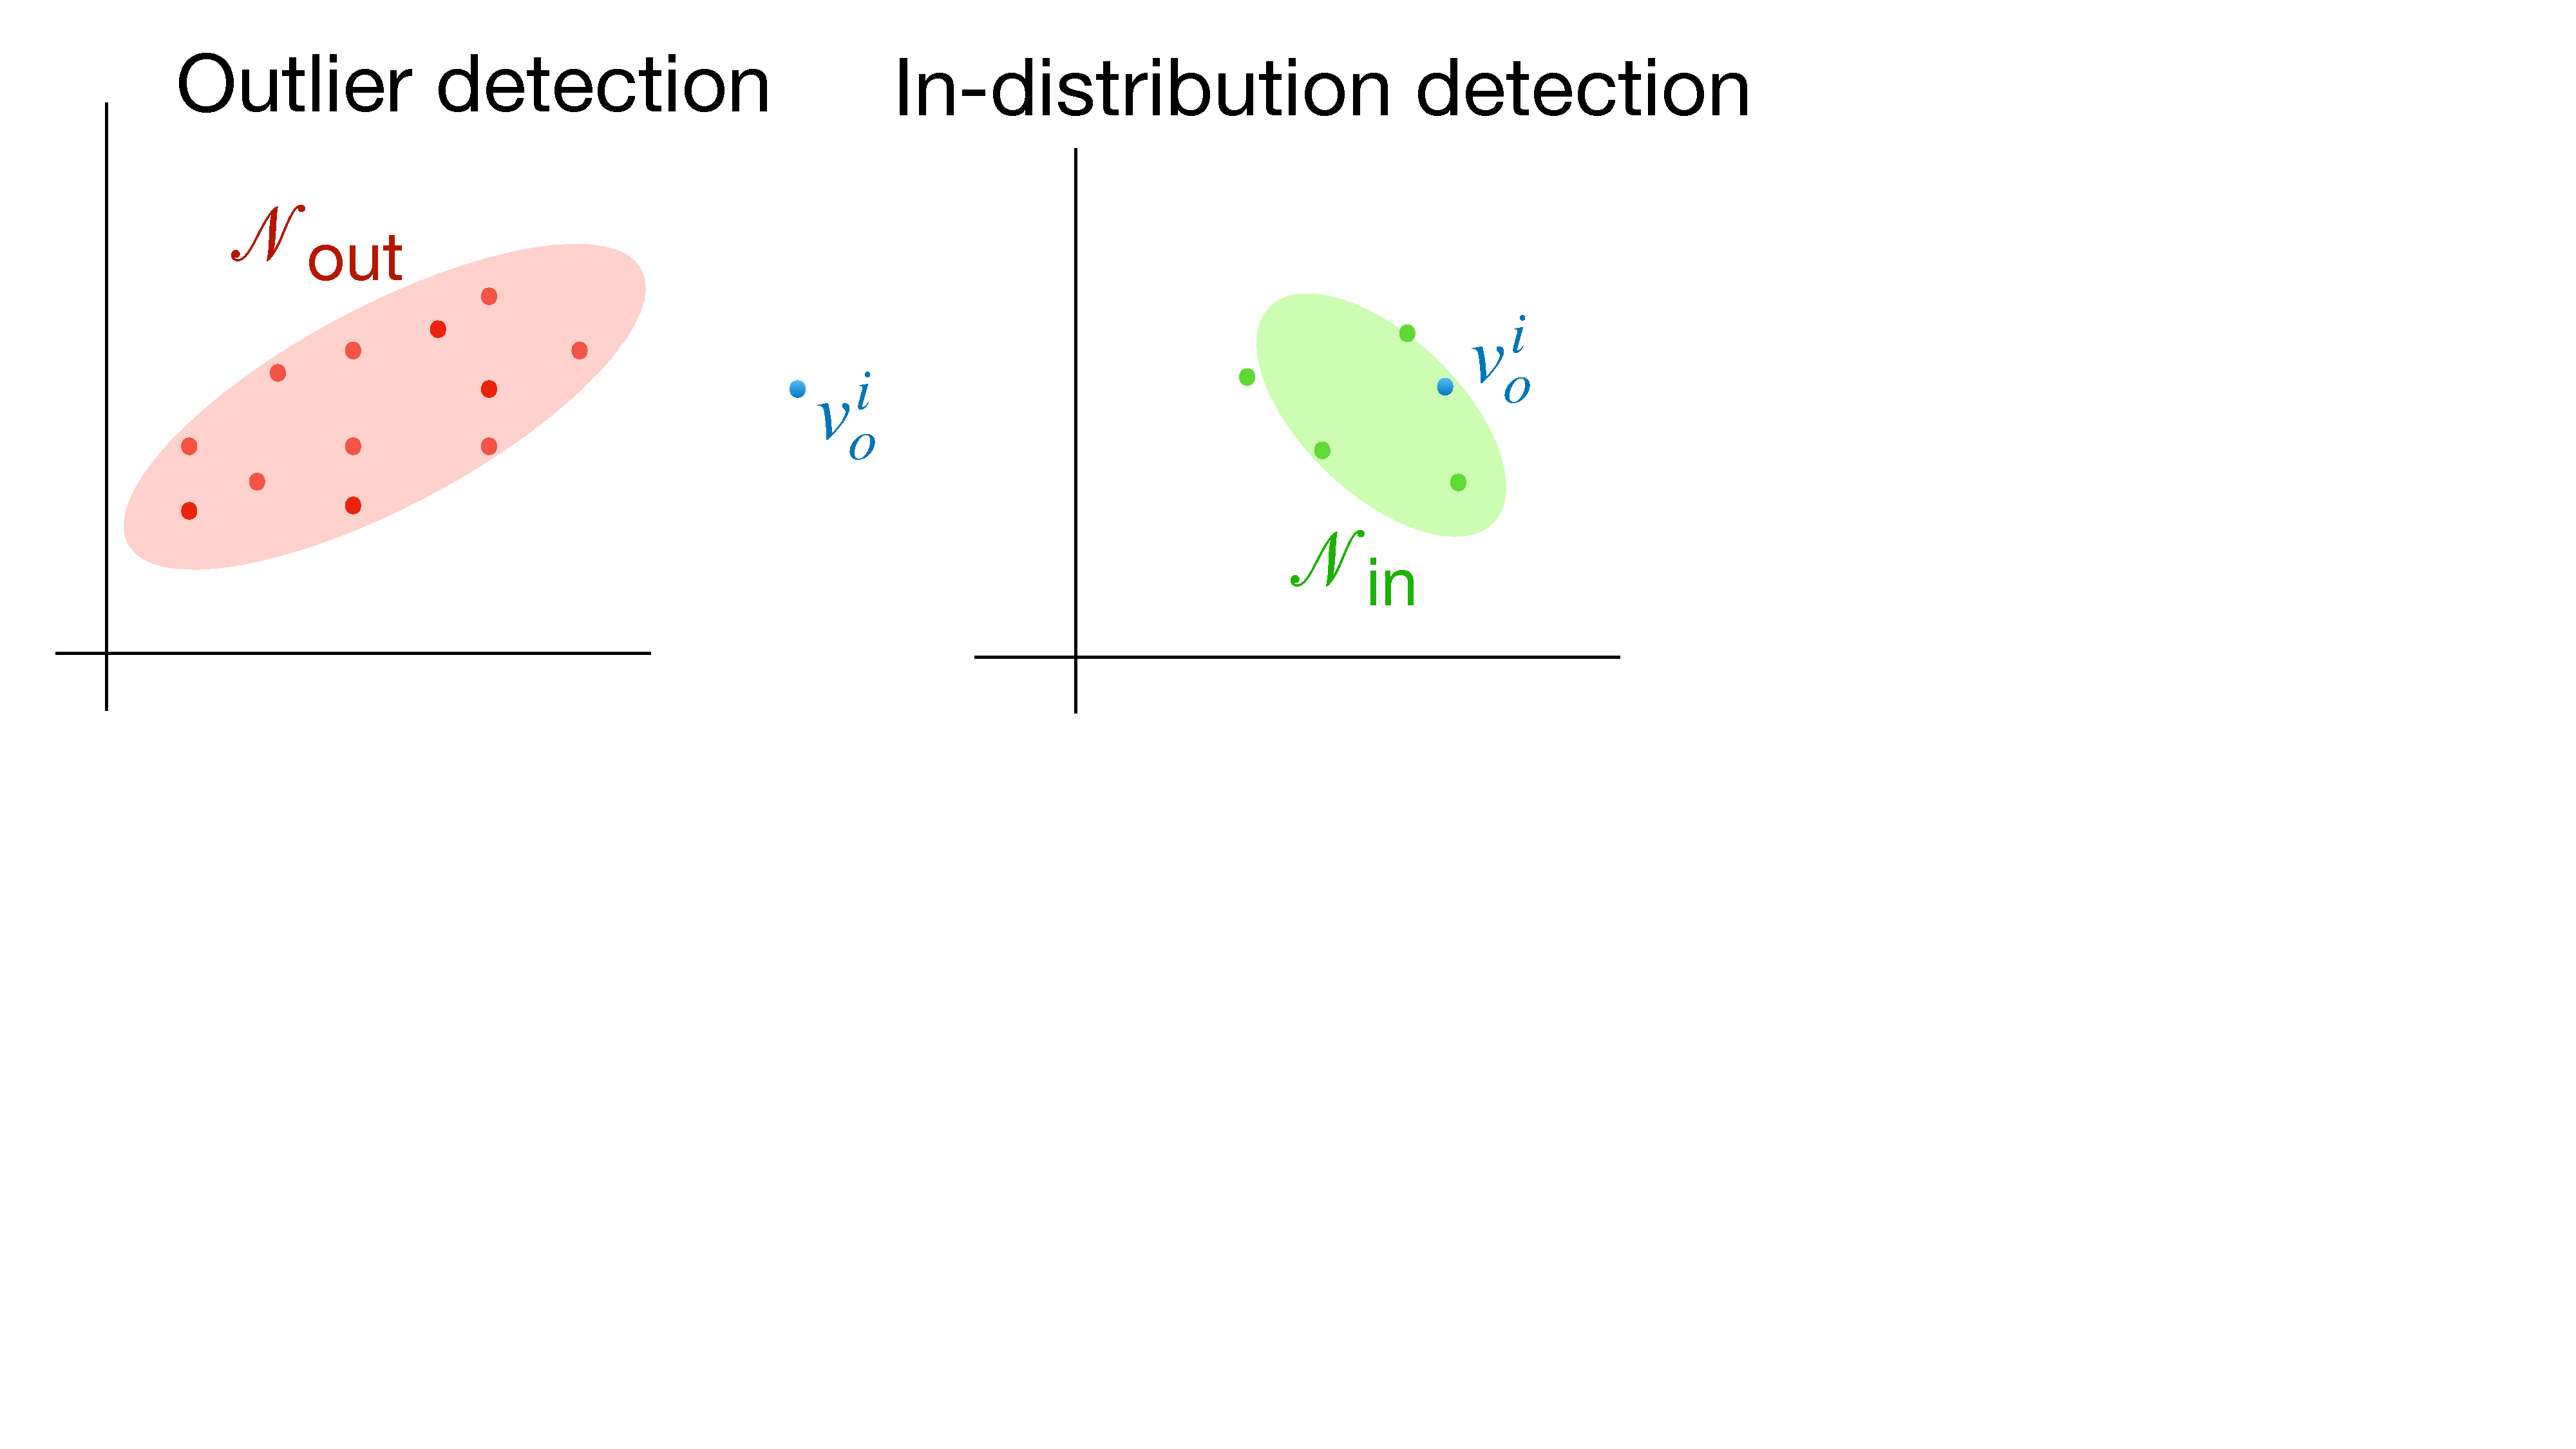
\includegraphics[width=0.9\columnwidth]{submissions/Ali2023/figures/outin.pdf}
      \caption{Two formulations for fact verification. Outlier detection samples a pool of non-existing facts and prioritizes objects that are outliers (left); in-distribution detection samples a pool of existing facts and prioritizes facts that are in-distribution samples to the pool (right).}
    \label{fig:met_out}
\end{figure}


\subsection{Out-of-distribution Sample Detection}
% \paragraph{Out-of-distribution sample detection non-existing facts with same head entity $v_s^i$ and relation $r_i$}
The first method considers a pool of non-existing facts with the same subject entity $v_s^i$ and relation $r^i$ as the related facts for the triplet $(v_s^i, r^i, v_o^i)$ in $\gE_\text{V}$.
We can formulate fact verification---especially verification of facts that might be missing---as an out-of-distribution sample detection task.
We can score the triplet $(v_s^i, r^i, v_o^i)$ by checking whether this is an ``outlier'' to the pool of non-existing facts. If it is an outlier, we may prioritize this triplet fact since it is more likely to be a True missing fact.
For each triplet in the given set of triplets $\gE_\text{V}: \{(v_s^1, r^1, v_o^1), \dots, (v_s^n, r^n, v_o^n)\}$, we score it in the following way against a set of related non-existing facts:
In order to score $(v_s^i, r^i, v_o^i)$, we first construct non-existing facts by replacing the objects of the query $(v_s^i, r^i, ?)$. We sample entities $v$ from KG as the object if $(v_s^i, r^i, v) \notin \gE$ using importance sampling, where the weight of each non-existing fact is proportional to the distance $p_{(v_s^i, r^i, v)}\propto\exp({\distt{v_s^i}{r^i}{v}})$ since we would like to sample non-existing facts with high confidence measured by the learned embeddings.
% Note this is sufficient in our use case and achieves empirically nice experimental results (detailed in \Secref{sec:experiment}), but one could design better negative sampling strategies \tocite{} to further improve fact pool. 
Assume we sample a pool of $k$ non-existing facts for the $i$-th triplet $(v_s^i, r^i, v_o^i)$, $\gP^i_\text{NE}: \{(v_s^i, r^i, v_1), \dots, (v_s^i, r^i, v_k)\}$ as well as the triplet fact $(v_s^i, r^i, v_o^i)$ to verify, we measure the delta using Mahalanobis distance-based confidence score. In detail, we estimate the mean and covariance of the entity embeddings of these negative samples $v_1, \dots, v_k$:
\begin{align}
    \vmu_\text{out}&=\frac{1}{k} \sum_j f_\theta(v_j) \nonumber\\
    \mSigma_\text{out}&=\frac{1}{k} \sum_j (f_\theta(v_j) - \vmu)(f_\theta(v_j) - \vmu)^\intercal,\label{eq:distribution_out}
\end{align}
which is the maximum likelihood estimation of the parameters of the multi-variate Gaussian distribution $\gN_\text{out}$.
We define the score $s_i$ of $(v_s^i, r^i, v_o^i)$ using the Mahalanobis distance between the embedding of and the Gaussian distribution $\gN_\text{out}$:
\begin{align}
    s_i = (f_\theta(v_o^i) - \vmu_\text{out})^\intercal \mSigma^{-1}_\text{out}(f_\theta(v_o^i) - \vmu_\text{out}).\label{eq:score_out}
\end{align}
Since large-scale KGs are often extremely sparse, we can easily construct a pool of $k$ non-existing facts with $k>1000$. In such a way, we can have an accurate estimation of the distribution $\gN_\text{out}$.
In order to identify the promising triplet facts, we formulate the problem as a binary classification task using the $s_i$, and prioritize ones with large $s_i$, which means that they are far from the $\vmu_\text{out}$ and likely to be a missing fact.

\subsection{In-distribution Sample Detection}
% \paragraph{Existing facts with same subject entity $v_s^i$ and relation $r_i$}
We can also approach the problem from the opposite perspective. Instead of scoring the fact $(v_s^i, r^i, v_o^i)$ using a set of related non-existing facts, we can score it using a set of existing facts with the same subject entity $v_s^i$ and relation $r^i$.  
For a given $(v_s^i, r^i, v_o^i)$, we find all answers $\gA_q$ to query $q=(v_s^i, r^i, ?)$ in the KG, and define the pool of related triple facts to be $\gP^i_\text{E}: \{(v_s^i, r^i, v_1), \dots, (v_s^i, r^i, v_k)\}$, where $v_1, \dots, v_k\in\gA_q$. 
Similarly, we can estimate a multivariate Gaussian distribution $\gN_\text{in}$:
\begin{align}
    \vmu_\text{in}&=\frac{1}{k} \sum_j f_\theta(v_j) \nonumber\\
    \mSigma_\text{in}&=\frac{1}{k} \sum_j (f_\theta(v_j) - \vmu)(f_\theta(v_j) - \vmu)^\intercal.\label{eq:distribution_in}
\end{align}
We define the score $s_i$ of $(v_s^i, r^i, v_o^i)$ using the Mahalanobis distance between the embedding of $v_o^i$ and the Gaussian distribution $\gN_\text{in}$:
\begin{align}
    s_i = (f_\theta(v_o^i) - \vmu_\text{in})^\intercal \mSigma^{-1}_\text{in}(f_\theta(v_o^i) - \vmu_\text{in}).\label{eq:score_in}
\end{align}
Since the pool of related facts are existing facts on the graph, we need to identify triplets with small score, which means that they are an in-distribution sample of the pool.
The key challenge of this method is that the estimation has high variance due to the limited number of answer size $|\gA_q|$. For example, the average number of answers for predicate \texttt{OccupationOf} is 1.32 in Wikidata. 

To improve the estimation accuracy we loosen the definition of related triple facts for $(v_s^i, r^i, v_o^i)$ by finding entities $v$ that are close to the subject entity $v_s^i$ in the embedding space. The intuition is that entities that are close in the embedding space share similar semantic meaning, \eg, the neighbors obtained by the Query2Box model for `Selena Gomez' node are all singer entities: including the nodes corresponding to `Taylor Swift', `50 Cent', `Miley Cyrus', `Halsey', and `Jay-Z'. Assume we find $m$ close entities of $v_s^i$: $\{v_1, \dots, v_m\}$, we collect the pool of existing related facts as the \emph{union} of all the triplet with one of the close entities as the subject and the relation of interest $r^i$ as the relation type, \ie, $\gP^i_\text{U}: \cup_{j=1}^m\:\{(v_j, r^i, v) | v\in\gA_q, q=(v_j, r^i, ?)\}$. 
We can tune the parameter $m$ to achieve a balance between computation efficiency and the accuracy of the estimation.
However, here we cannot simply use the previous framework, \ie, we cannot aggregate all the object entities in the pool and estimate the mean and covariance matrix only using the embeddings of the object entities as in \eqref{eq:distribution_in} and \eqref{eq:score_in}. The reason is that (1) there may be overlapping object entities, \ie, there exists an entity $v_\text{object}$ that is the object to multiple subject entities in the $\gP^i_\text{U}$, \ie, $\exists v_\text{object}, v_\text{subject}^1 \neq v_\text{subject}^2, \: (v_\text{subject}^1, r^i, v_\text{object}) \in \gP^i_\text{U}$ and $(v_\text{subject}^2, r^i, v_\text{object}) \in \gP^i_\text{U}$; (2) since the subject entities are different in the pool $\gP^i_\text{U}$, we need to \emph{align} the object entity $v_\text{object}$ with the subject entity $v_\text{subject}$ given a $(v_\text{subject}, r^i, v_\text{object})$ in the pool $\gP^i_\text{U}$. 

\begin{figure}
        \centering
      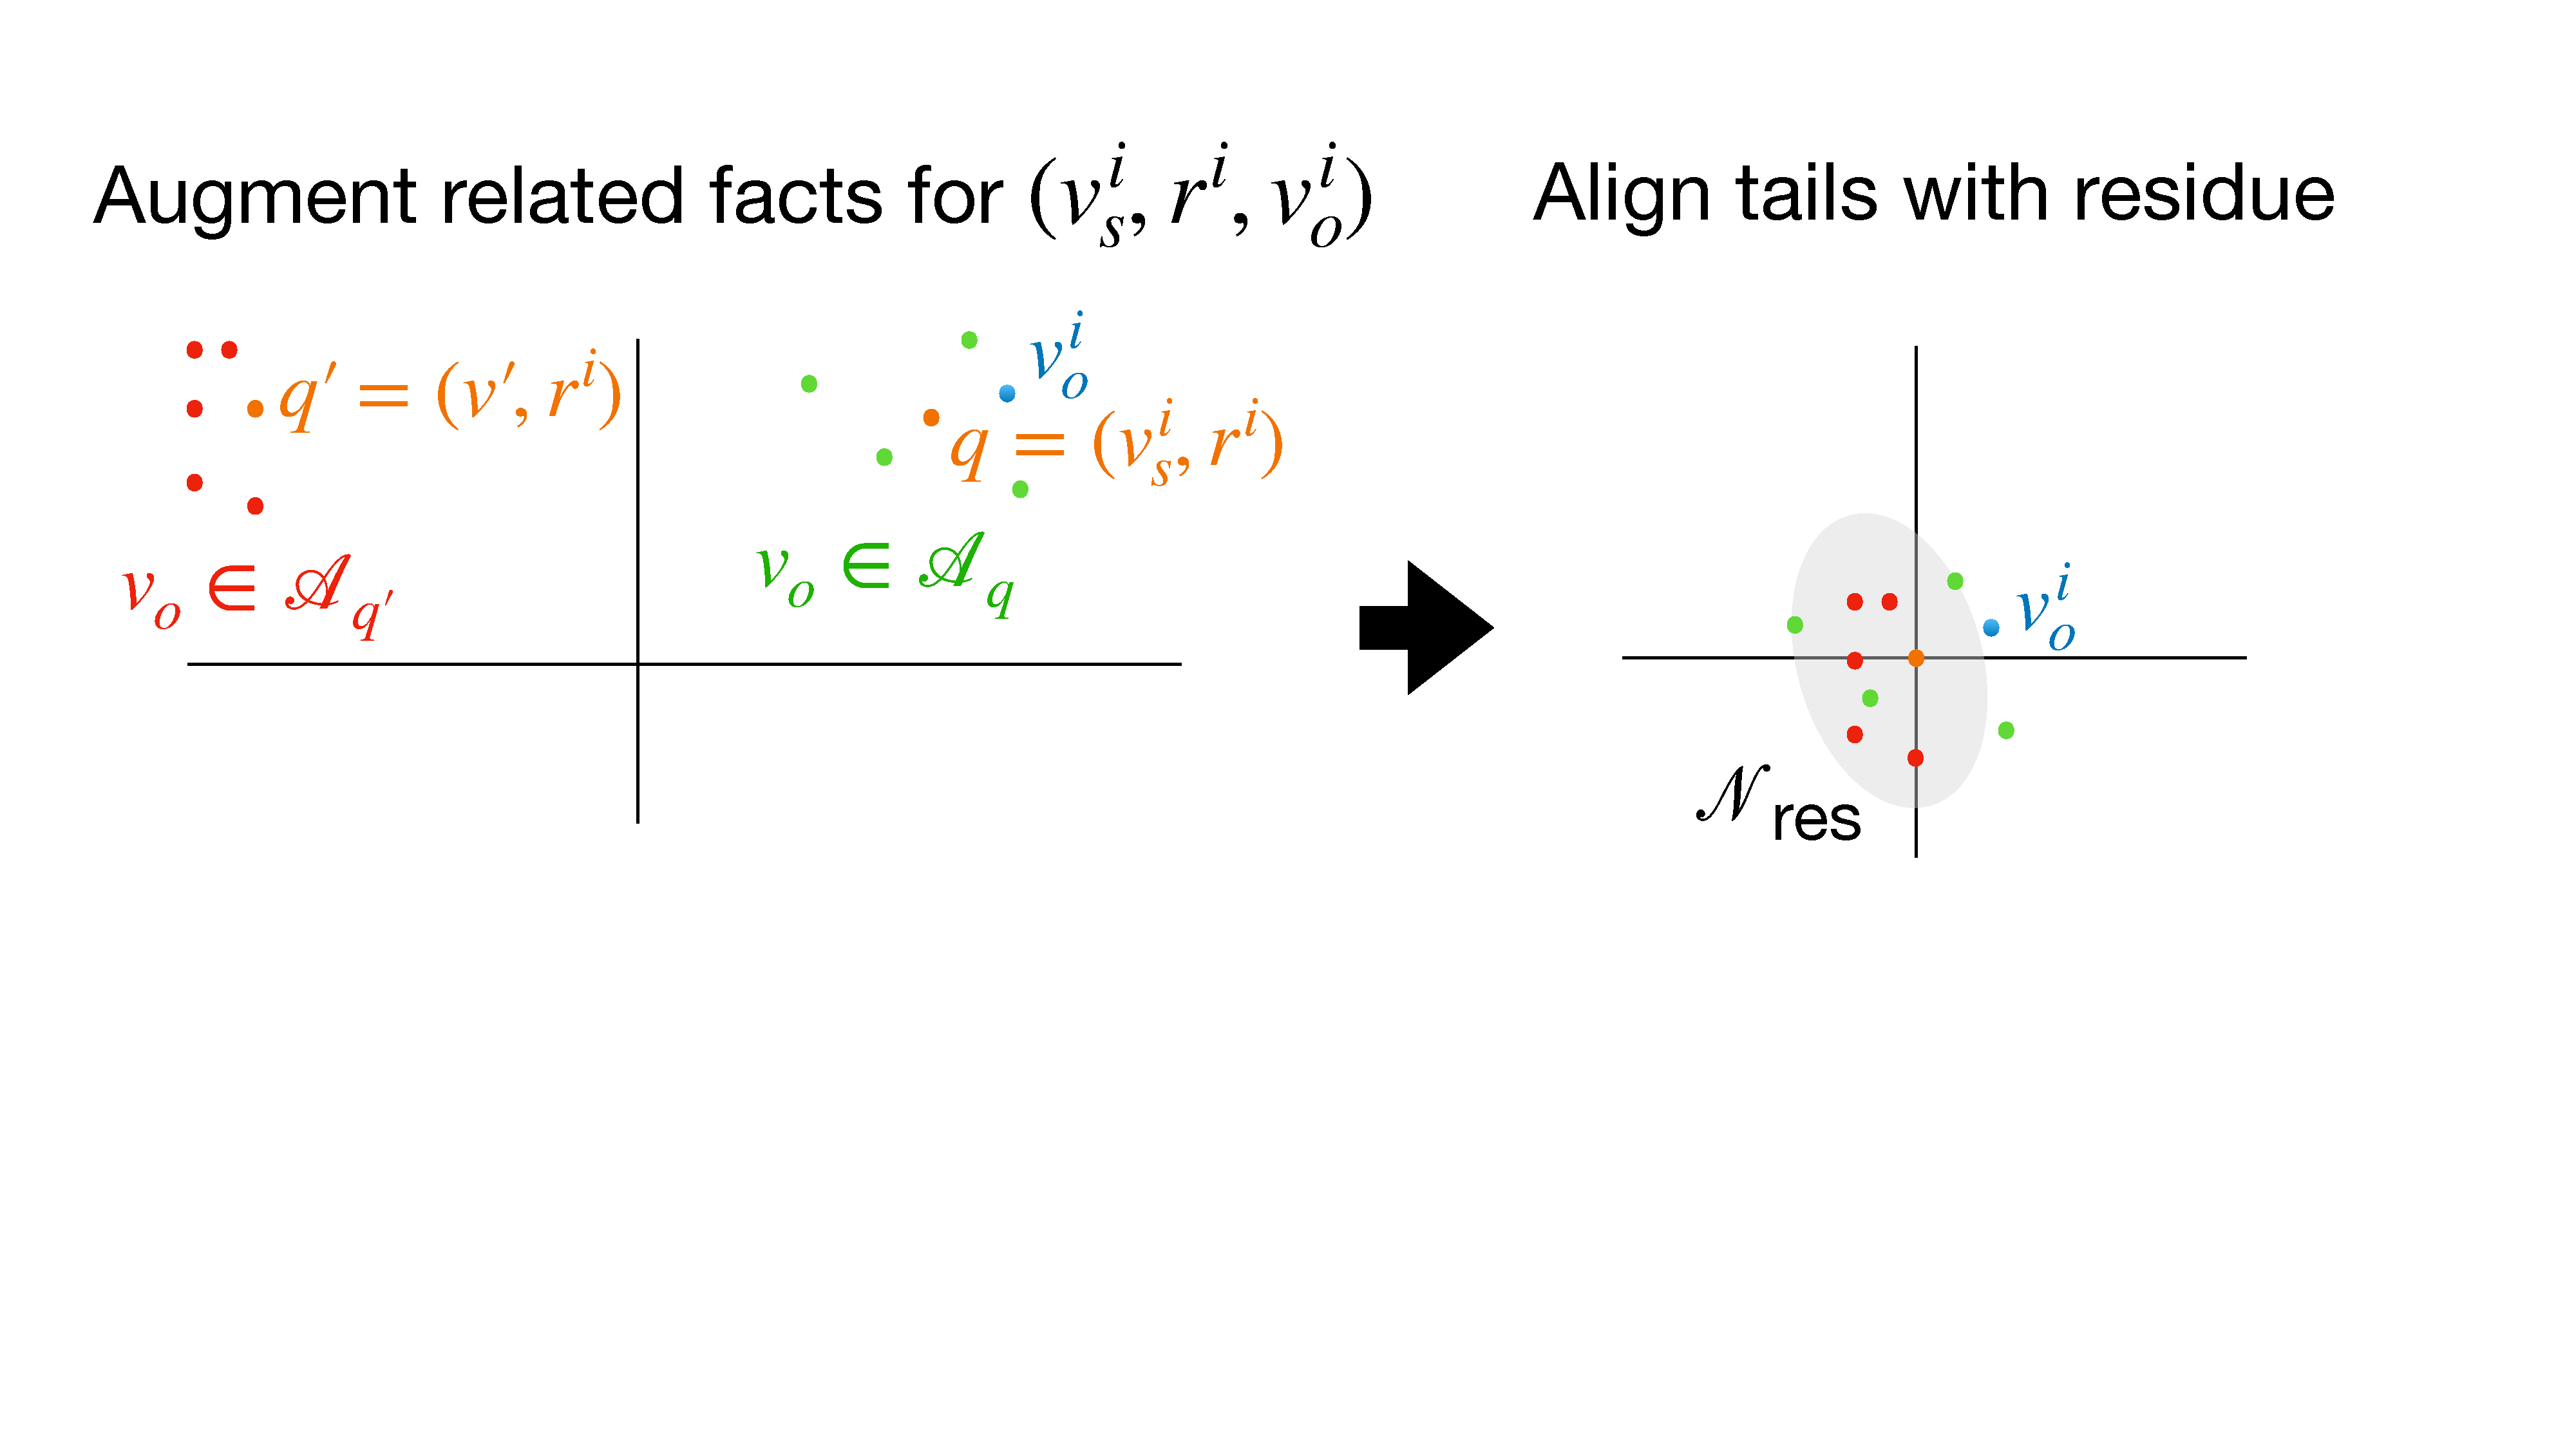
\includegraphics[width=\columnwidth]{submissions/Ali2023/figures/residue.pdf}
      \caption{In the in-distribution sample detection method, for a given fact $(v_s^i, r^i, v_o^i)$, we augment the pool of related facts by including facts with similar subject entities and the same relation $r^i$. As shown in the left Figure, we also consider facts $\{(v', r^i, v_o)\:|\:v_o\in\gA_q', q'=(v', r^i)\}$ as related facts. We align the object embeddings by finding the residue and estimate the $\gN_\text{res}$. We finally check whether the object $v_o^i$ is an in-distribution sample from $\gN_\text{res}$.}
    \label{fig:residue}
\end{figure}

Inspired by product quantization~\cite{jegou2010product}, here we align the object embedding by finding the residue between the query, \ie, the (subject, relation) pair $(v_\text{subject}, r^i)$ and the object entity $v_\text{object}$. Since the entity embeddings are high dimensional, the goal of this residue function is to capture the difference between the query and object \emph{along each dimension}. Different KG embedding methods may have different residue functions. Below we show the residue function of TransE with L1 distance for example.
\begin{align}
    \texttt{Residue}(v_s, r, v_o) = f_\theta(v_s) + f_\theta(r) - f_\theta(v_o).\label{eq:residue}
\end{align}
We emphasize that the residue function is different from the distance function in \eqref{eq:kgelossfunc}. The output of the residue function is a high-dimensional vector that represents the difference between a subject-relation pair and an object along each dimension, while \texttt{Dist} outputs a scalar distance.

Now given the related existing fact pool $\gP^i_\text{U}$ for triplet fact $(v_s^i, r^i, v_o^i)$, we first calculate the residue for each related fact in the pool: $\mathcal{S}^i_\text{U}: \{\texttt{Residue}(v_\text{subject}, r^i, v_\text{object}) | (v_\text{subject}, r^i, v_\text{object})\in\gP^i_\text{U}\}$, and then fit a multi-variate Gaussian distribution $\gN_\text{res}$:
\begin{align}
    \vmu_\text{res}&=\frac{1}{|\mathcal{S}^i_\text{U}|} \sum_{\vx\in\mathcal{S}^i_\text{U}} \vx \nonumber\\
    \mSigma_\text{res}&=\frac{1}{|\mathcal{S}^i_\text{U}|} \sum_{\vx\in\mathcal{S}^i_\text{U}} (\vx - \vmu)(\vx - \vmu)^\intercal.\label{eq:distribution_res}
\end{align}
Then we define the score $s_i$ using the Mahalanobis distance between the residue of $(v_s^i, r^i, v_o^i)$ and the Gaussian distribution $\gN_\text{res}$:
\begin{align}
    s_i = (\distr{v_s^i}{r^i}{v_o^i} - \vmu_\text{res})^\intercal \mSigma^{-1}_\text{res}(\distr{v_s^i}{r^i}{v_o^i} - \vmu_\text{res}).\label{eq:score_res}
\end{align}
We can prioritize facts with small $s_i$: although these facts do not exist in the graph, they are close to existing facts, so we should have human curators to verify these facts first.

\subsection{Distance Compared with Related Facts}
Besides the formulations of out-of-distribution/in-distribution sample detection, we also design a simple method that directly score the triplet $(v_s^i, r^i, v_o^i)$ by modeling the difference of the absolute distance of $(v_s^i, r^i, v_o^i)$ and the related facts.
Here we may reuse the definition of related facts as in previous sections, including non-existing facts with the same $v_s^i$ and relation $r^i$ as subject and relation, or existing facts with close subject entities and relation $r^i$.

Consider that we sample $k$ non-existing facts for the $i$-th triplet $(v_s^i, r^i, v_o^i)$: $\gP^i: \{(v_s^i, r^i, v_1), \dots, (v_s^i, r^i, v_k)\}$ as well as the triplet fact $(v_s^i, r^i, v_o^i)$ to verify, we formulate and measure the delta using the distance calculated by the embeddings. We calculate the distance $d_1=\distt{v_s^i}{r^i}{v_1}\in\R, \dots, d_k$, together with $d_t=\distt{v_s^i}{r^i}{v_o^i}$, and measure how $d_t$ is compared against $\{d_1, \dots, d_k\}$. We estimate a Gaussian distribution $\gN_\text{D}=(\mu_\text{D}, \sigma_\text{D})$ over the distances of non-existing facts $\{d_1, \dots, d_k\}$, and score $(v_s^i, r^i, v_o^i)$ by calculating how many standard deviations $d_t$ are away from the mean: $s_i=\frac{d_t - \mu_\text{D}}{\sigma_\text{D}}$. Here in order to identify the promising triplet facts, we prioritize ones with small $s_i$, which means that the distance of $(v_s^i, r^i, v_o^i)$ is considered much smaller than that of the related facts (estimated using $\gN_\text{D}$) and thus the triplet is likely to be a missing fact.

\subsection{Application to Verification of Existing Facts}
Above we introduced how we use our framework to solve one of the fact verification tasks, namely identifying the likely missing triplet facts. Another task that falls within the same domain is that we want to prioritize the existing triplet facts on the graph that are likely to be False. Our framework can be naturally adapted for this setting, where we can still collect related triplet facts, do outlier / in-distribution sample detection, or estimate a distribution of distance, and calculate how many standard deviations is this triplet fact away from the mean. Then we can use this score to identify and prioritize promising triplet facts in this setting.

\fi
\section{Scaling to Large KGs}\label{sec:system}
We discuss systems considerations when using KG reasoning embedding models over large-scale KGs. Beyond scalable training, we also require that inference over Query2Box models is scalable and incremental. This requirement is important to enable practical deployments over dynamic billion-scale KGs. We next discuss the main components of the architecture we adopt (see Figure~\ref{fig:sys_overview}).

 \begin{figure}
        \centering
      \includegraphics[width=0.7\columnwidth]{submissions/Ali2023/figures/embedding_models_q2box_v2.pdf}
      \caption{An overview of using Knowledge Graph Embedding models for large-scale fact ranking.}
    \label{fig:sys_overview}
\end{figure}

The multi-hop nature of embedding models such as Query2Box poses unique challenges when training these models over billion-scale KGs. In the case of shallow KG embedding models, graph partitioning is a common method for scaling training~\cite{zhu2019graphvite, lerer2019pytorch}. Unfortunately, these methods are not applicable in the case of reasoning-based embeddings. When using Query2Box it is important that we can generate training samples by performing multi-hop traversals of the graph. Such traversals can span multiple partitions. At the same time, it is not always practical to pre-compute such samples in advance. To alleviate this issue, we opt for a single-machine multi-GPU deployment during training and leverage the recently introduced SMORE engine~\cite{ren2021smore} to perform training. SMORE provides a mixed GPU-CPU solution that leverages both the main memory and GPU memory to scale training. In addition, training examples are generated on the fly thus avoiding unnecessary pre-compution. Indicative throughput measurements and scaling of SMORE is shown in Figure \ref{fig:speedup}. A requirement here is that the machine have sufficient main and on-device memory to store the entire graph and thus avoid partitioning. While this requirement is satisfied by modern hardware configurations it is a cost-hungry option. We believe disk-based or distributed training of reasoning-based KG embeddings is an exciting research direction. Once training is complete, the embedding models are archived and then used for inference.

\begin{figure}[t]
\centering
    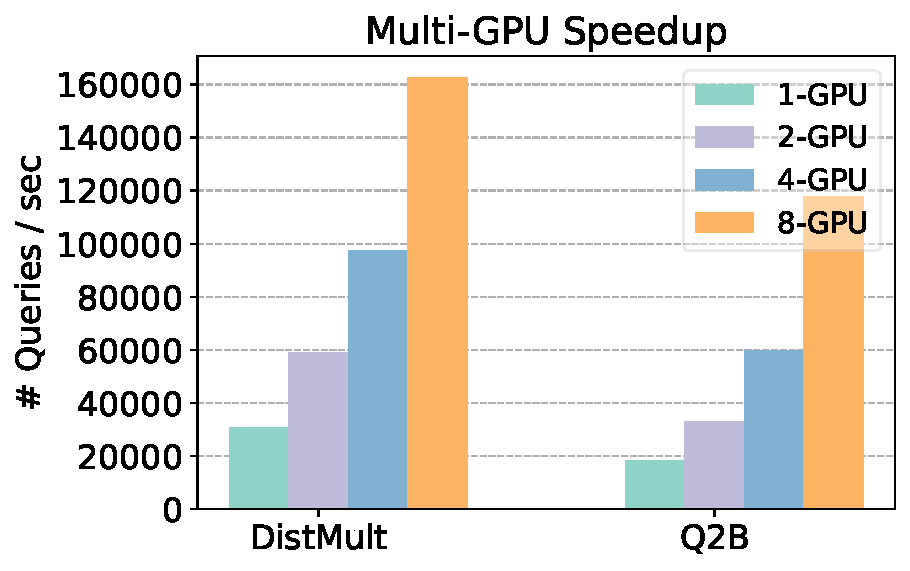
\includegraphics[width=0.3\columnwidth]{submissions/Ali2023/figures/wiki-speedup.pdf}
    \caption{Multi-GPU scaling of SMORE for training the DistMult and Query2box embedding models.
    }
\label{fig:speedup}
\end{figure}

At inference time, we opt for a batch inference setting. We first compute a series of candidate queries that correspond to the set of facts that we want to enable ranking over. We leverage a computation graph engine to materialize all \emph{candidate} queries (\ie, \texttt{(subject, predicate, object} triples) and use the learned Query2Box model to obtain a score for each query. The number of candidate facts can exceed the size of the original KG as we consider multiple subject, object configurations that may not appear in the original graph. To deal with the volume of generated queries we opt for a scatter gather-based multi-GPU inference across multiple machines in a GPU cluster. The trained model is loaded in the executor allocated to each machine and the candidate facts are partitioned across machines. The corresponding inference results are gathered into a single relational store and then used for downstream processing. Given the stability of the Query2Box representations (see Section~\ref{sec:experiment}), we maintain the fact ranking results via periodic retraining of the Query2Box models followed by batch inference. Inference results for fact ranking are versioned across different training and batch inference runs.

\iffalse

\revise{
Performing batch inference for related entity search (Section \ref{sec:related_entities}) has additional requirements due to the unique characteristics of the related entity search task: (i) hybrid queries and their relational predicates require inference techniques beyond traditional vector similarity search-based solutions, and (ii) the volume and variety of candidate queries that are generated from available prior workloads render static, ``one size fits all'' solutions ineffective. 
To this end, we employ \hybridindex~\cite{mohoney2023high} hybrid vector similarity search system for  batch inference over KG embeddings, which provides the following suite of optimizations for \textit{high-throughput batch processing of hybrid queries}:
}

% The batch processing requirement of our workload is in fundamentally different from the existing industrial-scale systems focus on latency optimized online hybrid query processing. Therefore, in contrast to the other fact ranking tasks, our primary challenge here is performing \textit{high-throughput batch processing of hybrid queries} on KG embedding trained for the use-case. The requirements of related entity search use-case necessitate new optimizations that current vector database systems do not cover. To this end, we proposes the following suite of solutions including a \emph{workload-aware vector index} and a \emph{multi-query optimization technique}:

\textbf{Workload-aware vector index:}
First, we introduce a new workload-aware index for vector databases.
Specialized vector indexes that either partition the data or form multi-level indexes over centroids are commonly used in vector databases to speed-up vector similarity search \cite{guo2022manu, wang2021milvus, yang2020pase}. Here, we use past workload information to guide the partitioning of the vectors in the underlying index in a  way that hybrid queries can be answered by accessing as few partitions as possible. We extend the concept of \emph{query-data routing trees (qd-trees)}~\cite{qd-tree} to consider both vectors and relational predicates from a hybrid query workload when generating physical data layout at data loading time. The resulting data layout partitions the vectors using the distribution of the attributes associated with vectors, the attribute constraints, and similarity of vectors present in the hybrid query workload. We then use the resulting partitioning scheme to generate an index layout that enables us to process a batch workload of hybrid queries by accessing vectors from as few partitions as possible.

\textbf{Batch query optimization:}
Second, we introduce a multi-query optimization technique that (i) batches queries with similar attribute and vector similarity constraints; and (ii) performs batch vector distance computation against a posting list of vectors obtained from a clustering-based index over the vectors. 
This optimization is motivated by the fact that the set of candidate queries are computed from past user queries and evaluated in a batch setting, which enables computation sharing across queries.
% This optimization is motivated by the fact that our target hybrid query workloads need to be evaluated in a batch setting, enabling computation sharing across queries. 
Note that this optimization is orthogonal to the workload-aware vector index and is applicable to any clustering-based vector index.

\fi
% \begin{figure*}[]

% % \subfloat{%
% %   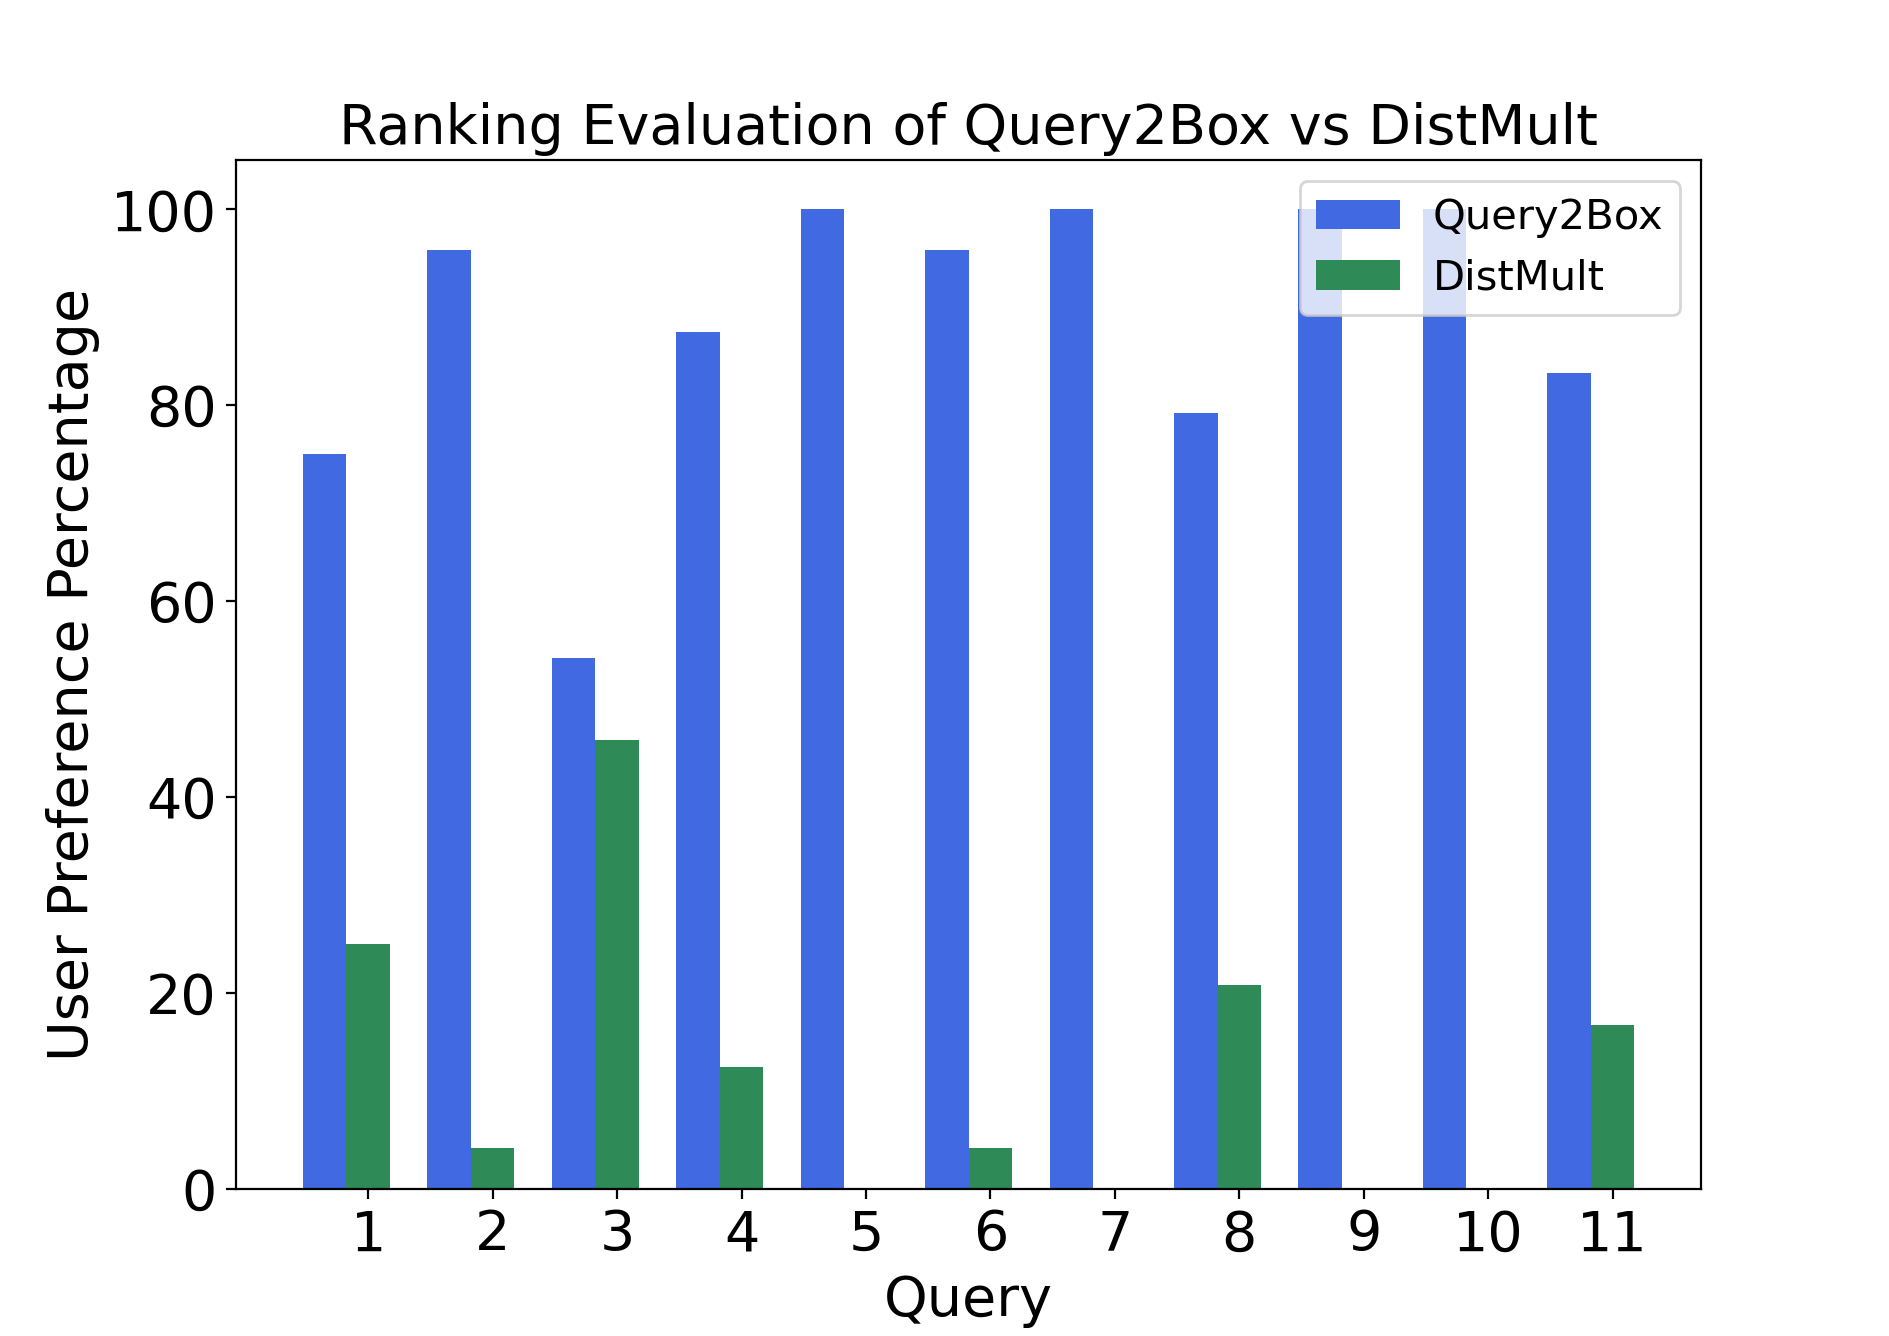
\includegraphics[clip,width=0.75\columnwidth]{submissions/Ali2023/figures/q2b_distmult.png}%
% % }
% \subfloat{%
%   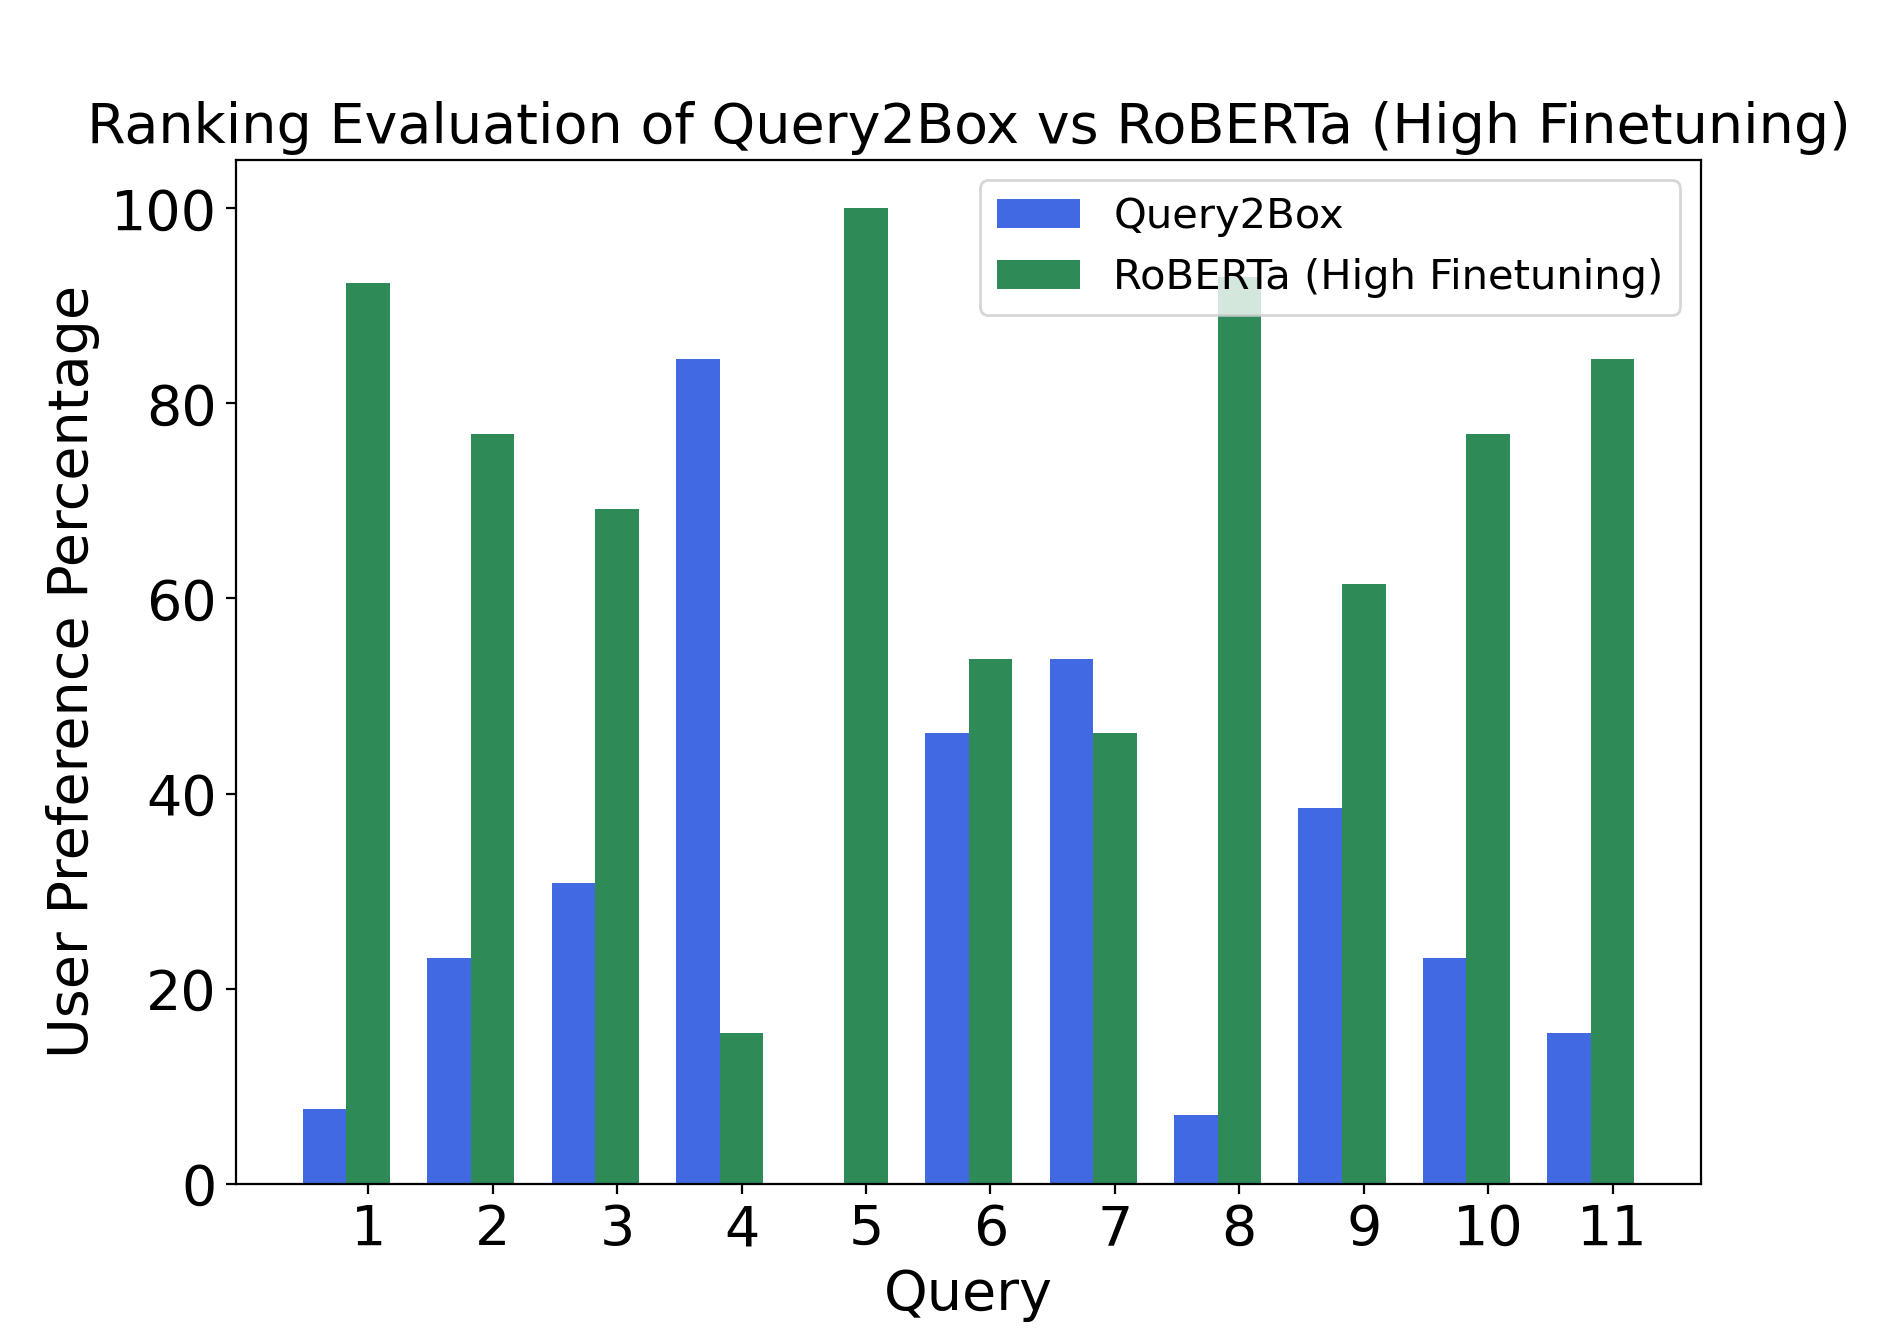
\includegraphics[clip,width=0.65\columnwidth]{submissions/Ali2023/figures/q2b_r1.png}%
% }
% ~
% \subfloat{%
%   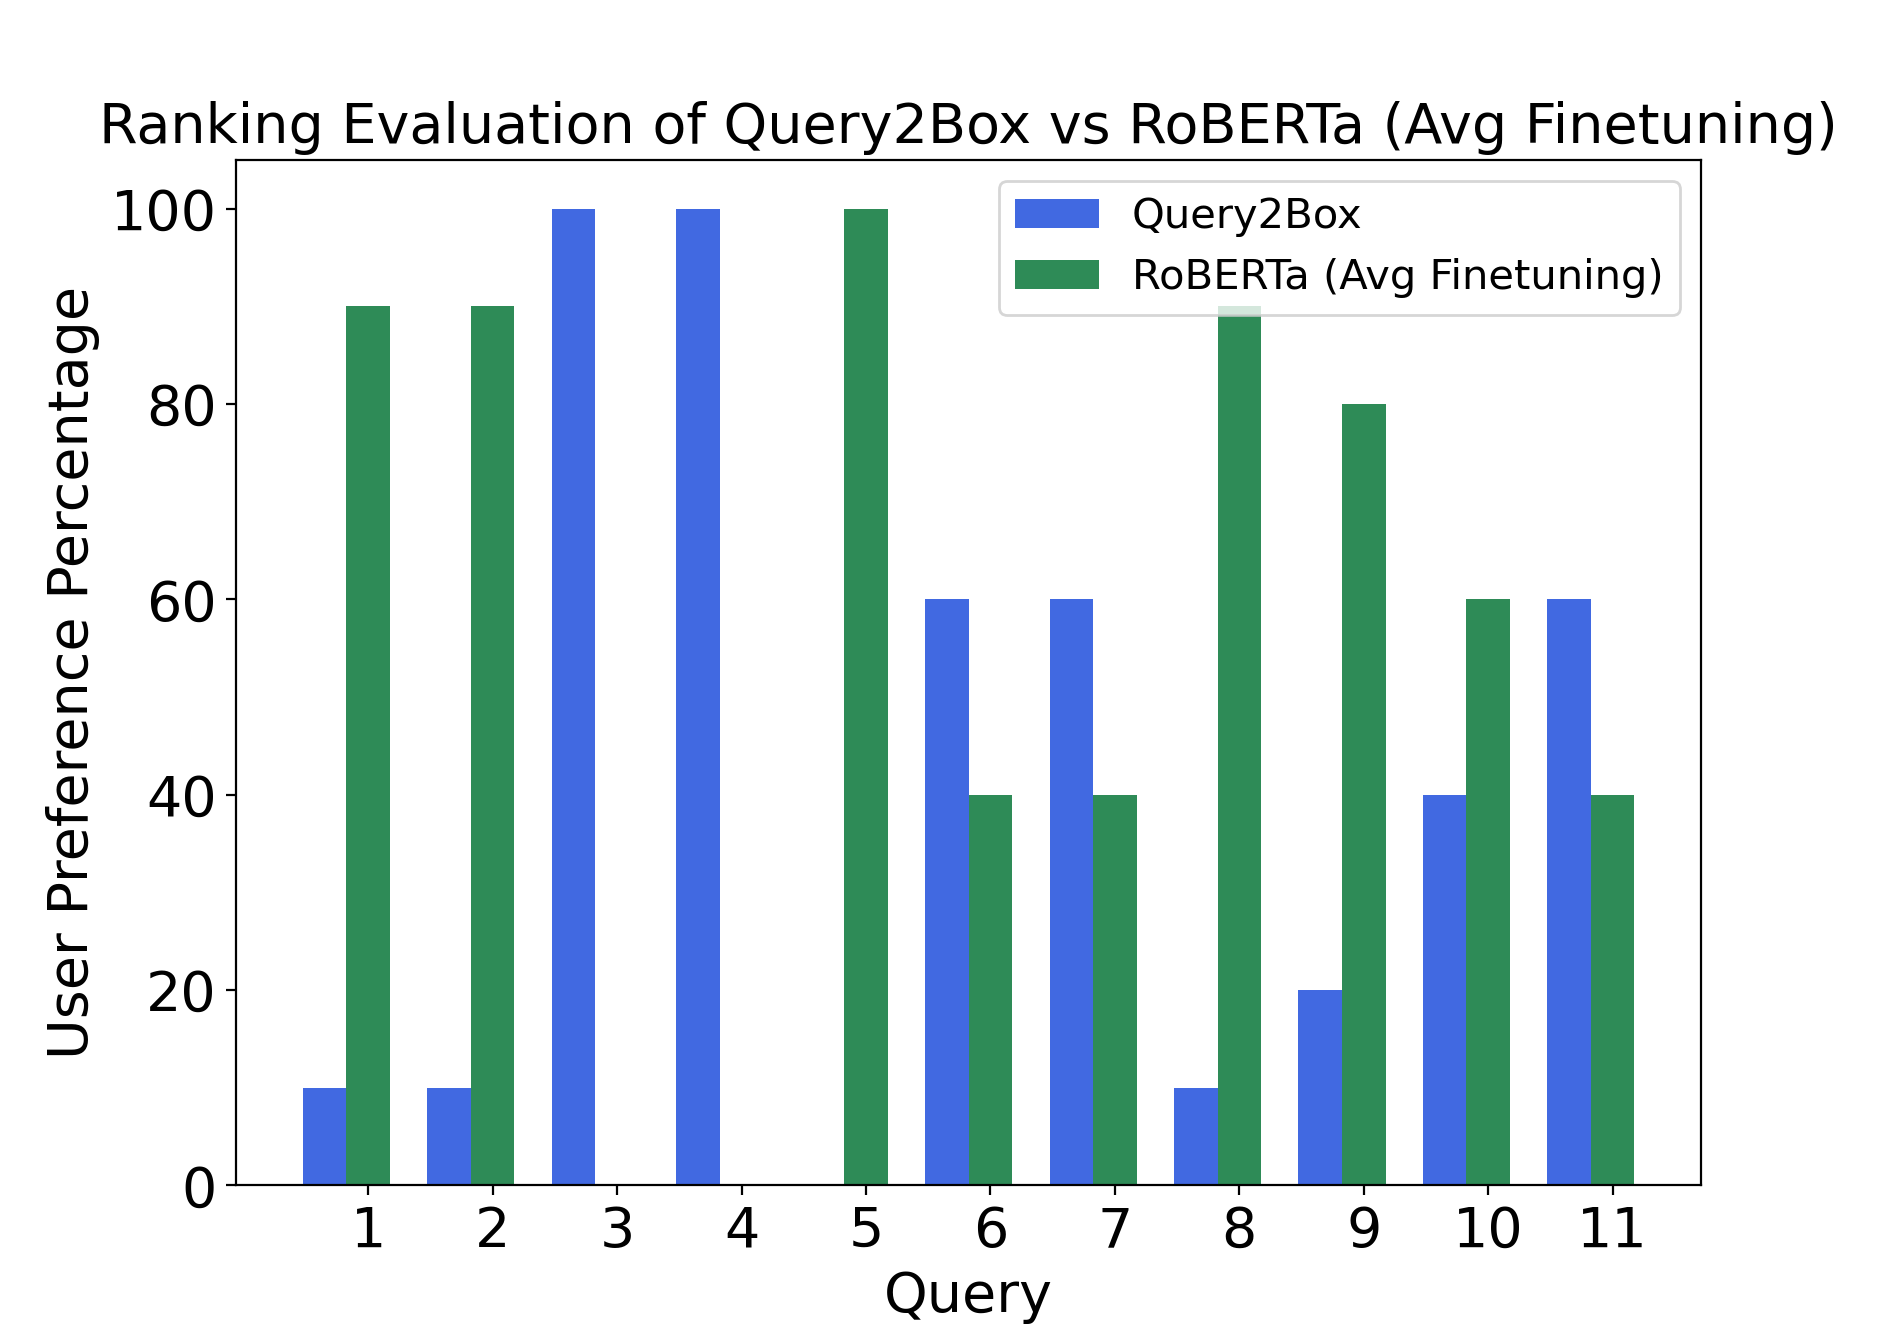
\includegraphics[clip,width=0.65\columnwidth]{submissions/Ali2023/figures/q2b_r2.png}%
% }
% ~
% \subfloat{%
%   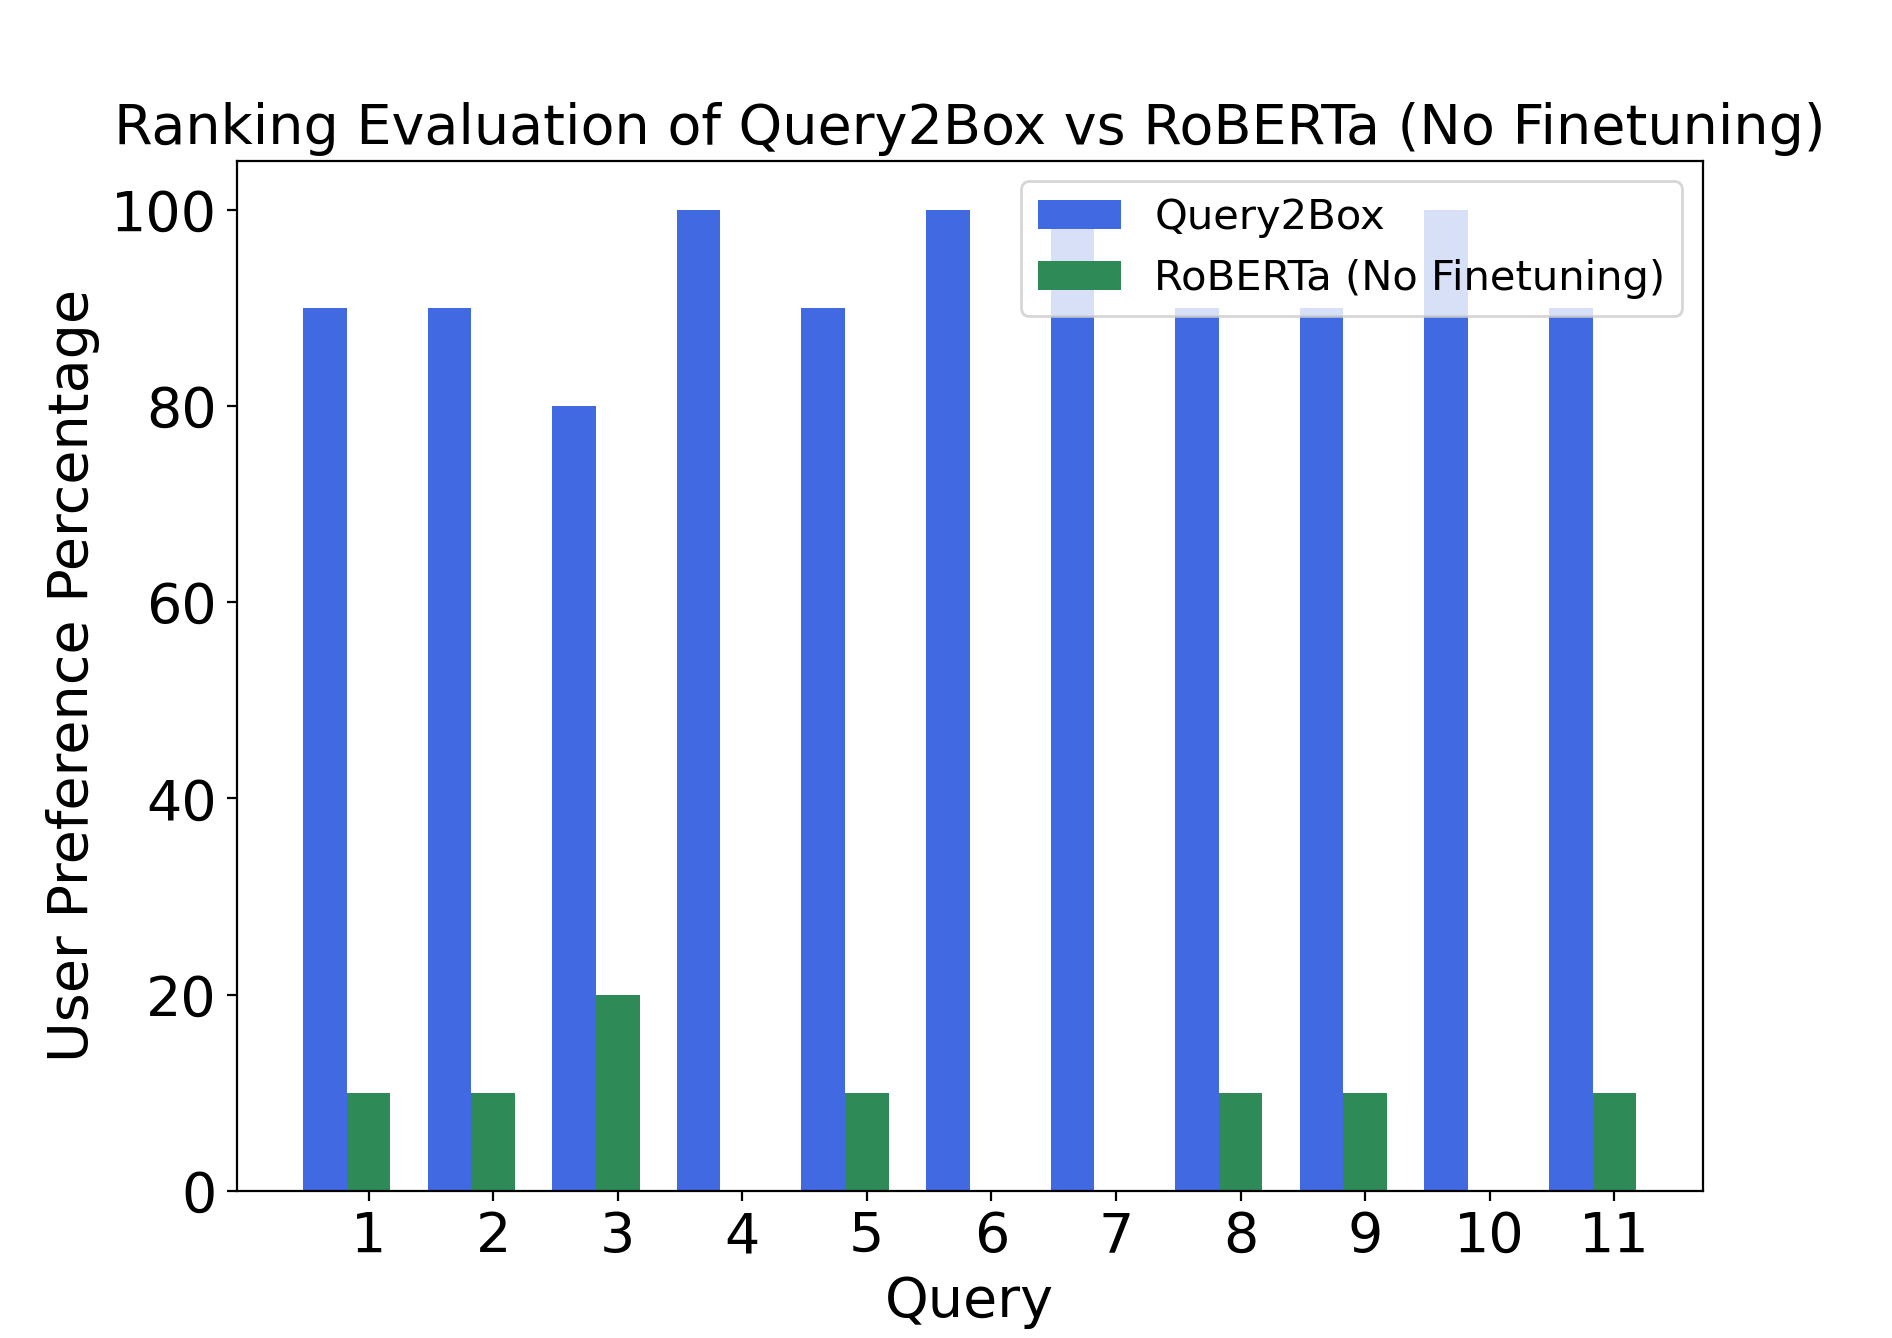
\includegraphics[clip,width=0.65\columnwidth]{submissions/Ali2023/figures/q2b_r3.png}%
% }
% \caption{Fact ranking using Query2Box vs. RoBERTa.}

% \label{fig:q2b_roberta}

% \end{figure*}

\begin{figure*}[!t]
\centering
\begin{minipage}{0.86\textwidth}
\begin{tabular}{@{}c@{}c@{}}
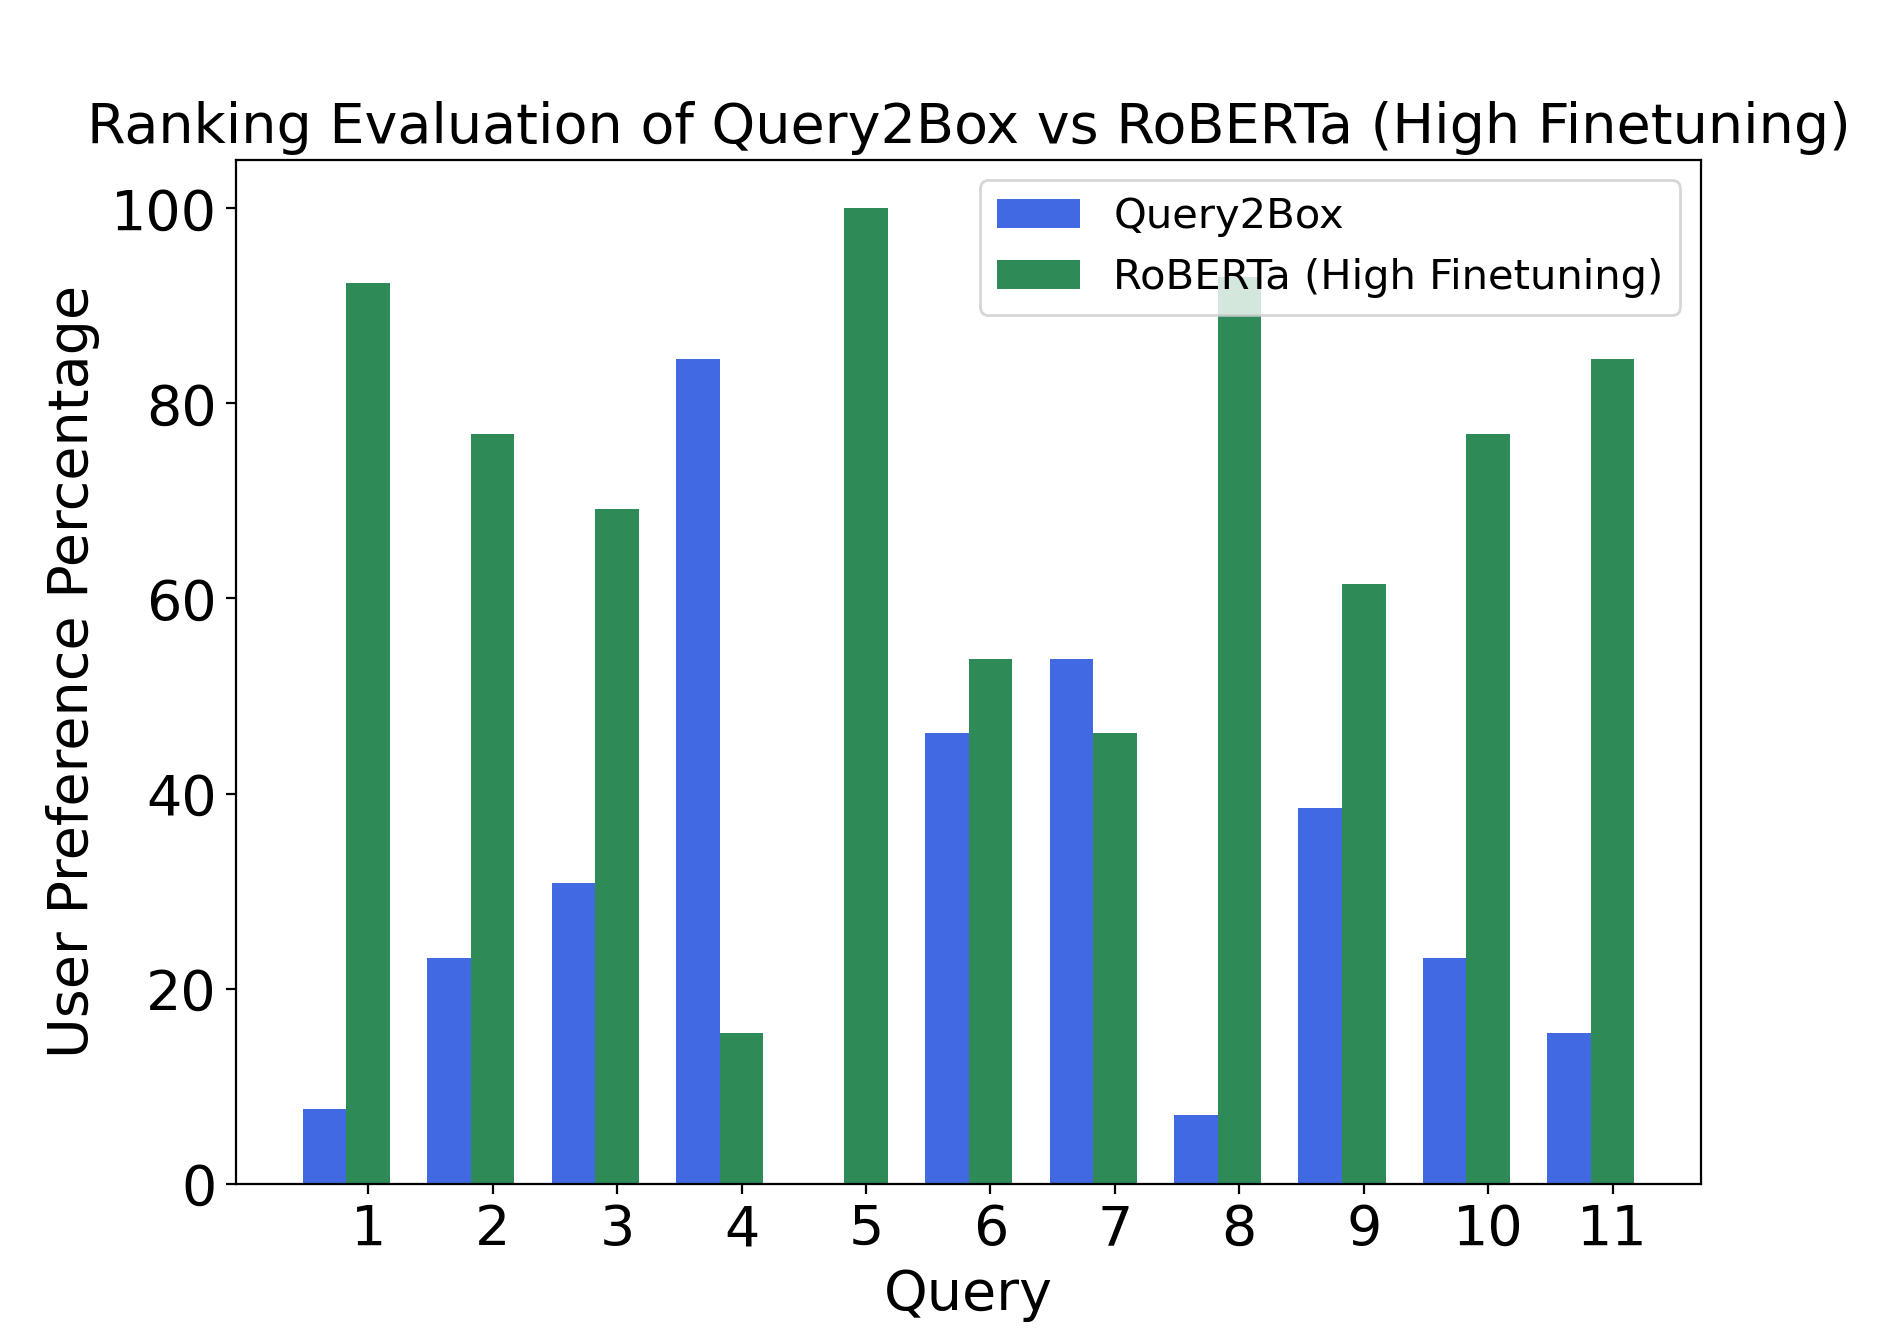
\includegraphics[width=0.43\textwidth]{submissions/Ali2023/figures/q2b_r1.png} & 
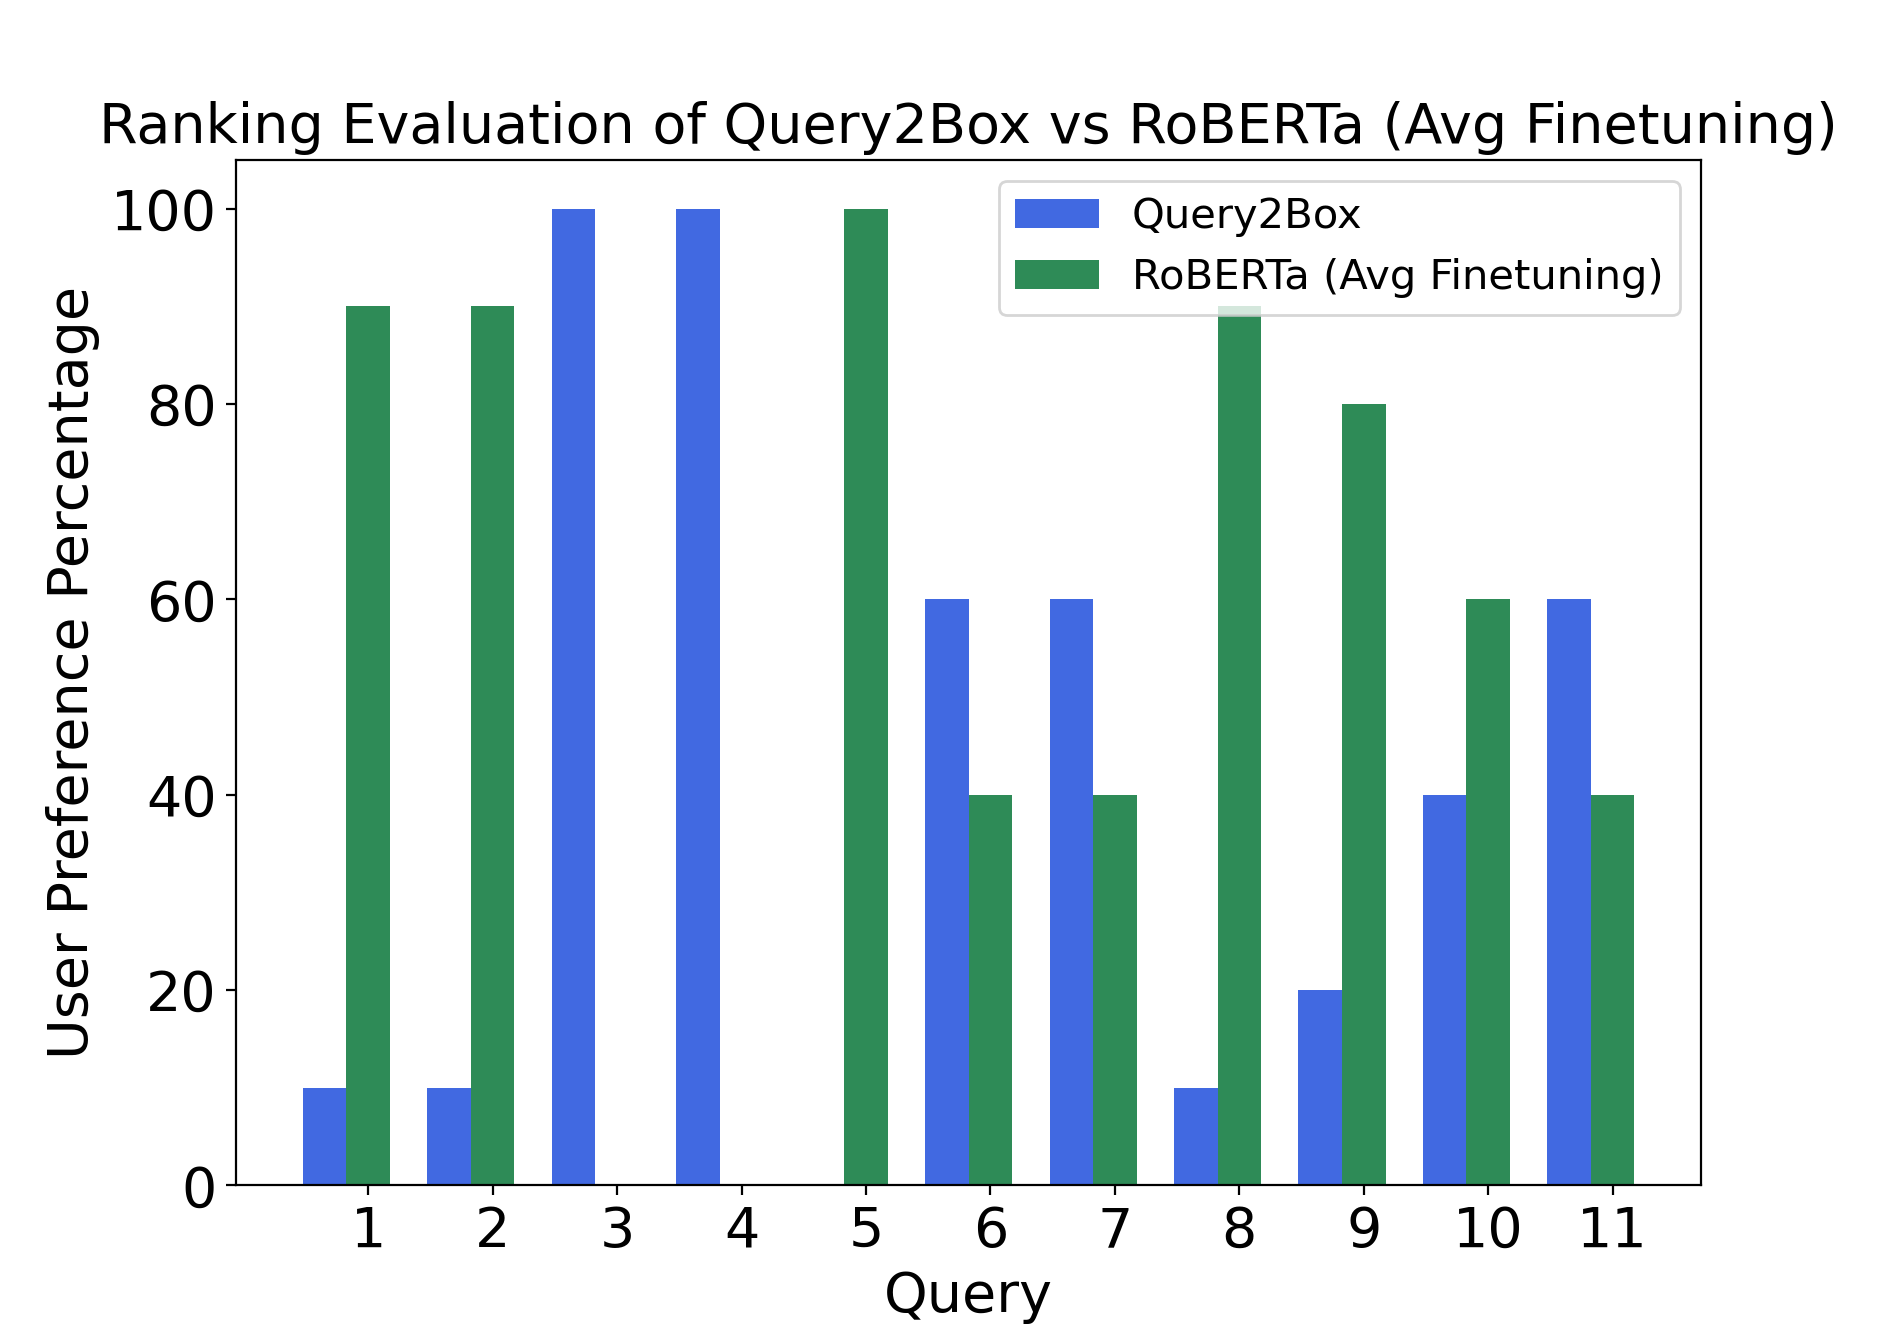
\includegraphics[width=0.43\textwidth]{submissions/Ali2023/figures/q2b_r2.png} \\
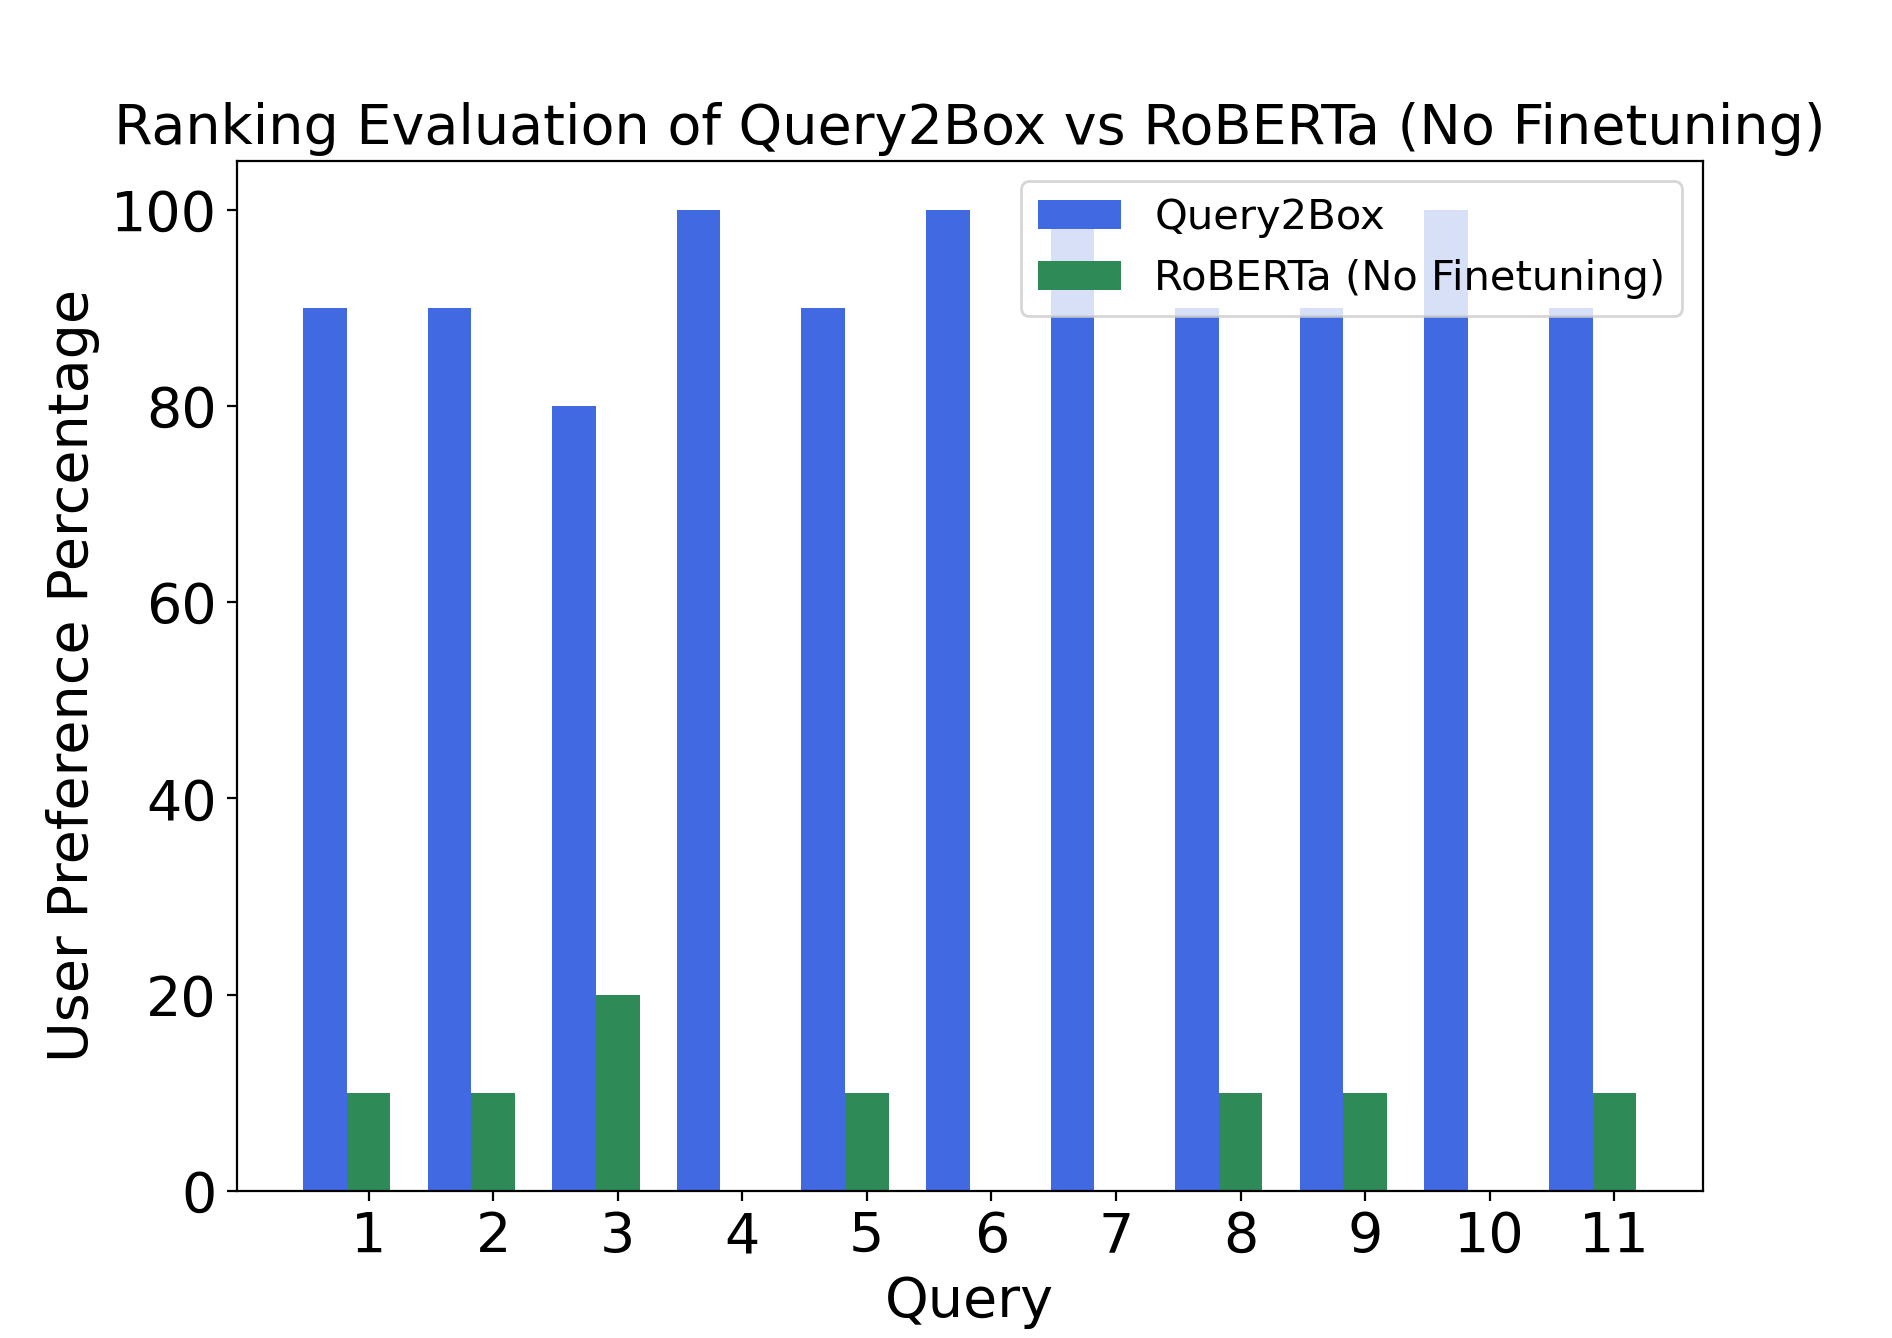
\includegraphics[width=0.43\textwidth]{submissions/Ali2023/figures/q2b_r3.png} &
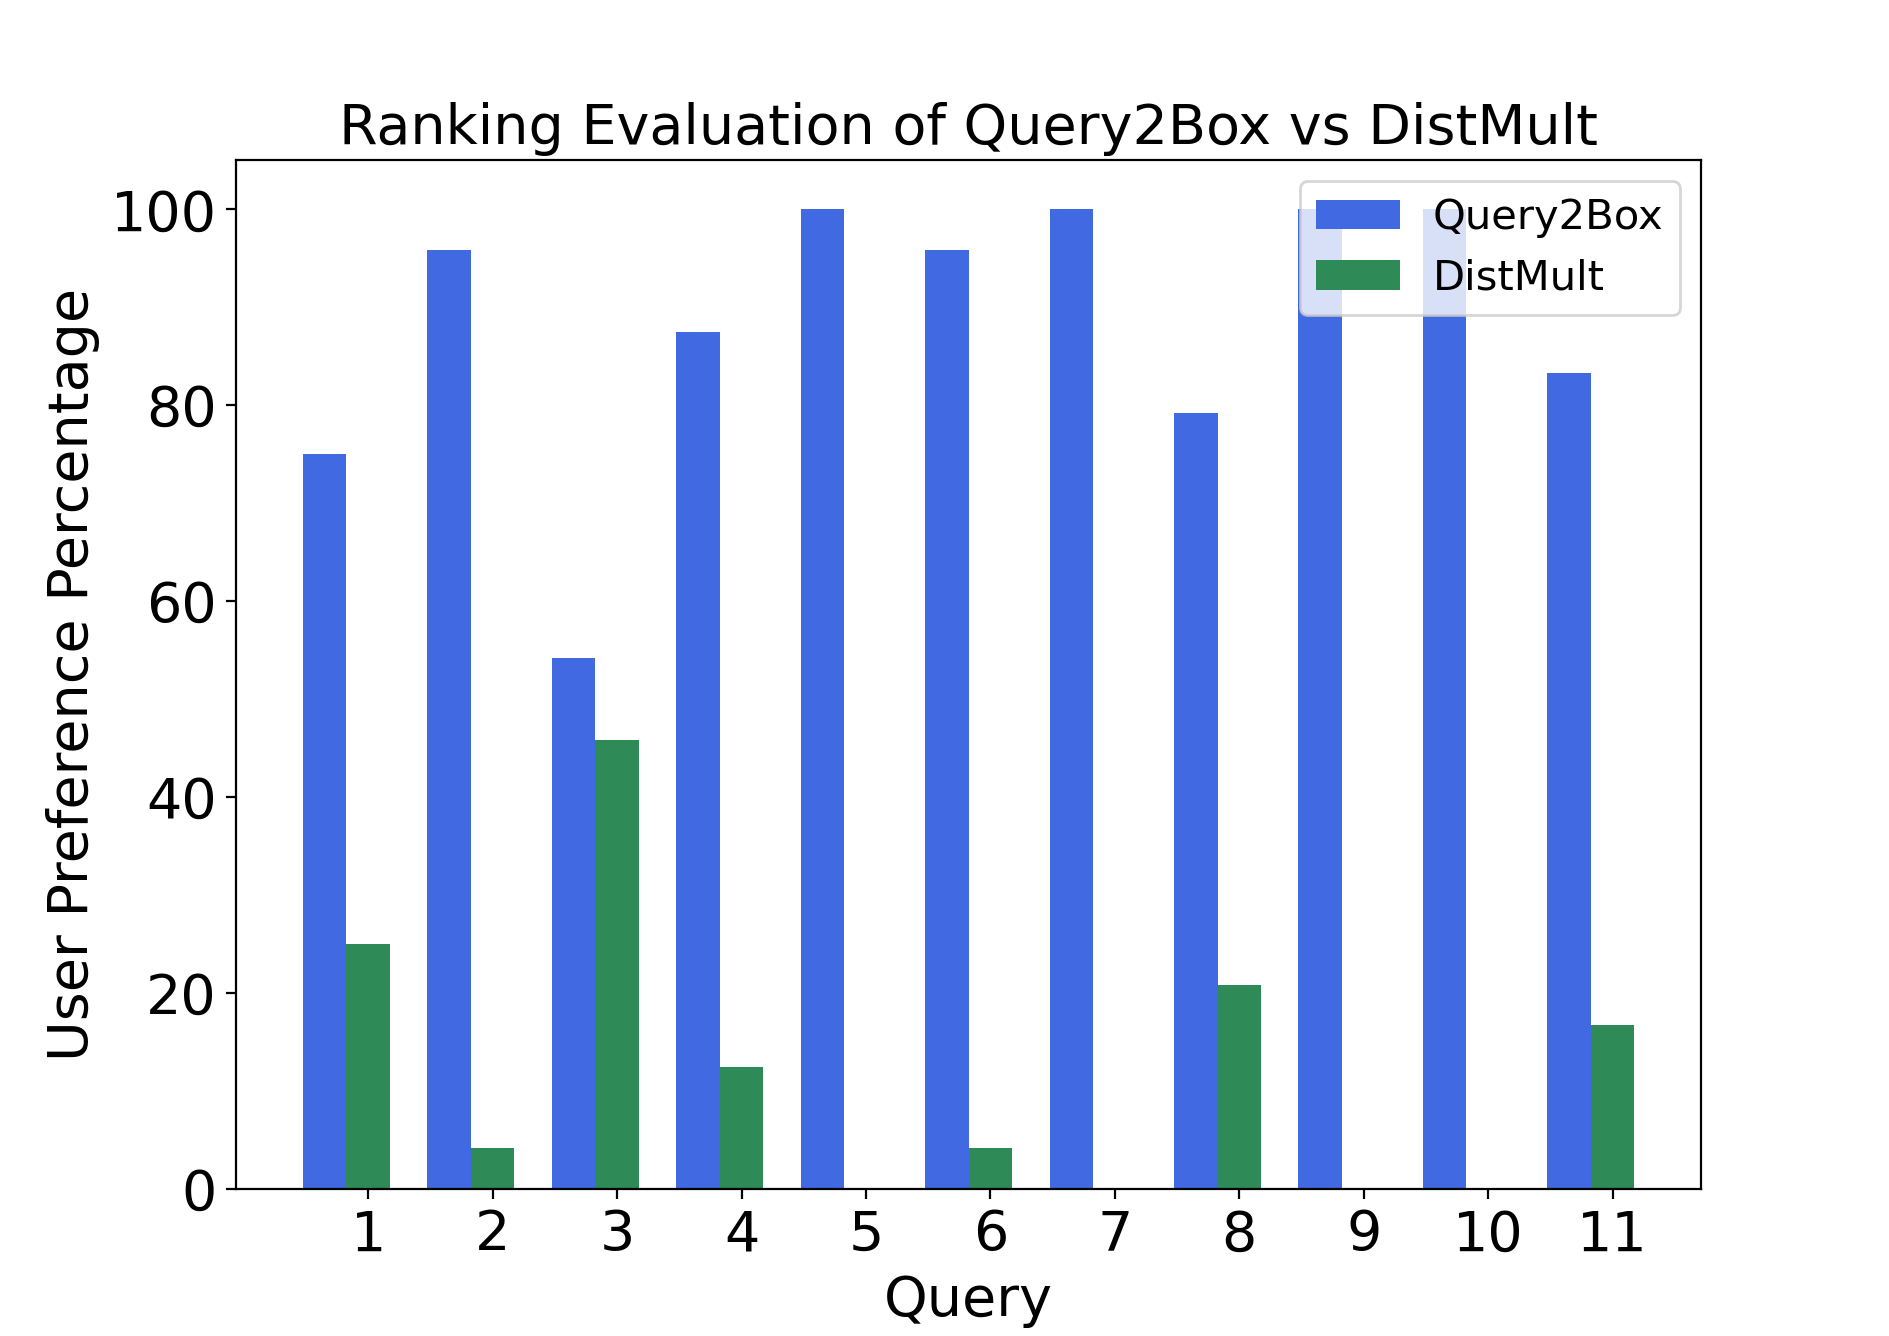
\includegraphics[width=0.43\textwidth]{submissions/Ali2023/figures/q2b_distmult.png}
\end{tabular}
\vspace{-3mm}
\caption{Fact ranking using Query2Box vs. RoBERTa and Query2Box vs. DistMult.
\label{fig:q2b_roberta_distmult}}
\end{minipage}
\end{figure*}







\begin{table}[t]
\caption{Average user preference (based on results in Figures \ref{fig:q2b_roberta_distmult}) for Q2Box vs other methods for different tasks. For RoBERTa models, (H): high finetuning, (A): average finetuning, (N): no finetuning.\label{tab:jen_ranking}}
\begin{tabular}{ccccc}
\textbf{Query2Box} & \textbf{DistMult} & \textbf{RoBERTa (N)} & \textbf{RoBERTa (A)}      & \textbf{RoBERTa (H)}      \\
\hline
1- TV Actor        & 1- Film Actor     & 1- Singer            & 1- Film Producer & 1- Actor         \\
2- Film Actor      & 2- Singer         & 2- Film Producer     & 2- Film Director & 2- Singer        \\
3- Film Director   & 3- Film Director  & 3- Film Director     & 3- Film Actor    & 3- Film Producer \\
4- Actor           & 4- Film Producer  & 4- Film Actor        & 4- TV Actor      & 4- Film Director \\
5- Film producer   & 5- Actor          & 5- Actor             & 5- Actor         & 5- Film Actor    \\
6- Singer          & 6- TV Actor       & 6- TV Actor          & 6- Singer        & 6- TV Actor     
\end{tabular}
\end{table}

\begin{table}[t]
\centering
\caption{Average user preference (based on results in Figure \ref{fig:q2b_roberta_distmult}) for Q2Box vs other methods for different tasks. For RoBERTa models, (H): high finetuning, (A): average finetuning, (N): no finetuning.}
\label{tab:avg_ranking}
\small
\begin{tabular}{@{}lccc@{}}
\textbf{Comparison Task} & \textbf{Competitor} & \textbf{Competitor Avg. Percentage} & \textbf{Q2Box Avg. Percentage} \\
\hline
DistMult / Q2Box         & DistMult            & 12\%                     & \textbf{88\%} \\
RoBERTa (H) / Q2Box      & RoBERTa (H)         & \textbf{70\%}            & 30\%          \\
RoBERTa (A) / Q2Box      & RoBERTa (A)         & \textbf{57\%}            & 43\%          \\
RoBERTa (N) / Q2Box      & RoBERTa (N)         & 7\%            & \textbf{93\%}          \\
\end{tabular}
\end{table}



% \begin{table*}[]
% \small
% \center
% \caption{Stability results of fact ranking. Query2box consistently achieves better performance than DistMult.}\label{tab:stability}
% \begin{tabular}{|l|c|c|c|c|ccc|}
% \hline
% \multicolumn{1}{|c|}{\multirow{2}{*}{}} & \multirow{2}{*}{Kendall} & \multirow{2}{*}{Weighted Kendall} & \multirow{2}{*}{Set-based Overlap} & \multirow{2}{*}{Rank-biased Overlap} & \multicolumn{3}{c|}{AdaptiveTau}                           \\ \cline{6-8} 
% \multicolumn{1}{|c|}{}                  &                          &                                   &                                    &                                      & \multicolumn{1}{c|}{0.02}  & \multicolumn{1}{c|}{0.05}  & 0.1   \\ \hline
% DistMult                                & 0.380                    & 0.384                             & 0.962                              & 0.990                                & \multicolumn{1}{c|}{0.460} & \multicolumn{1}{c|}{0.498} & 0.484 \\ \hline
% Query2box                               & \textbf{0.854}                    & \textbf{0.868}                             & \textbf{0.990}                              & \textbf{0.997}                                & \multicolumn{1}{c|}{\textbf{0.877}} & \multicolumn{1}{c|}{\textbf{0.917}} & \textbf{0.943} \\ \hline
% \end{tabular}
% \end{table*}



\begin{table}[!t]
\small
\center
\caption{Stability results of fact ranking. Query2box consistently achieves better performance than DistMult.}\label{tab:stability}
\begin{tabular}{cccccccc}
          & Kendall        & \begin{tabular}[c]{@{}c@{}}Weighted\\ Kendall\end{tabular} & \begin{tabular}[c]{@{}c@{}}Set-based\\ Overlap\end{tabular} & \begin{tabular}[c]{@{}c@{}}Rank-biased\\ Overlap\end{tabular} & \begin{tabular}[c]{@{}c@{}}AdaptiveTau\\ $\delta'=0.02$\end{tabular} & \begin{tabular}[c]{@{}c@{}}AdaptiveTau\\ $\delta'=0.05$\end{tabular} & \begin{tabular}[c]{@{}c@{}}AdaptiveTau\\ $\delta'=0.1$\end{tabular} \\ \hline
DistMult  & 0.380          & 0.384                                                      & 0.962                                                       & 0.990                                                         & 0.460                                                                & 0.498                                                                & 0.484                                                               \\
Query2Box & \textbf{0.854} & \textbf{0.868}                                             & \textbf{0.990}                                              & \textbf{0.997}                                                & \textbf{0.877}                                                       & \textbf{0.917}                                                       & \textbf{0.943}                                                     
\end{tabular}
\end{table}


\section{Experiments}\label{sec:ali_experiment}
We evaluate reasoning-based KG embeddings for fact ranking. We focus on fact ranking tasks that align with use cases in industrial deployments. We evaluate the following aspects of our proposed framework: (1) the utility to end users when using KG embeddings for fact ranking, (2) the stability of KG embedding models and hence to what extent they satisfy deployment requirements.

\subsection{Experiment Setup}

\newparagraph{Queries and Facts}
We focus on queries of the format \qu{What is the occupation of \texttt{[Celeb\_Name]}?} which captures the ranking task. We rank possible object completions for the structured query $(v_s, \texttt{OccupationOf}, ?)$, where $v_s$ is the entity of interest. Our dataset contains several million queries obtained by real intelligent assistant user queries.

\newparagraph{Knowledge Graph}
We consider the entire Wikidata KG~\cite{wikidata} to validate the proposed framework. The version of Wikidata that we use contains 1,754,058,566 facts defined over 91,900,599 entities and 35,446 relation types. We train our framework on this KG and obtain the answers to the aforementioned set of user queries by finding entities in this KG.

\newparagraph{Baselines}
We evaluate a diverse array of methods, including KG reasoning embeddings \textit{Query2box}~\cite{ren2020query2box}, shallow KG embeddings \textit{DistMult}~\cite{distmult},  and masked language models (MLMs) \textit{RoBERTa}~\cite{liu2019roberta}. 

For KG embedding based methods, both DistMult and Query2box fit in our unified framework. We adopt the standard training procedures for these models (see Section~\ref{sec:ali_prelim}). \iffalse Specifically, we randomly initialize the entity embedding matrix $\rmV_\theta$ and the relation embedding matrix $\rmR_\theta$ for both models. \fi For DistMult, we sample existing edges as positive samples and non-existing edges as negative samples to train the DistMult model with the objective defined in \eqref{eq:kgelossfunc}, where the distance and residue functions are defined in \Secref{sec:ali_prelim}. For Query2box, similar to~\cite{ren2020query2box} and as discussed in \Secref{sec:ali_background}, we sample multi-hop queries (\Figref{fig:query}), and their answers and non-answers to optimize the contrastive objective in \eqref{eq:lossfunc}. Besides the entity and relation embedding matrices, we use the neural logic operators in Query2box to embed the complex queries and optimize the query embeddings such that they are close to the answer embedding and pushed far away from the embedding of the sampled non-answers. We use the distance function of the original Query2box model and design the residue function as described in \Secref{sec:ali_prelim}.








For both DistMult and Query2Box, we use SMORE~\cite{ren2021smore} for training. We train both for 100k iterations with the Adam optimizer~\cite{kingma2014adam}. We anneal the learning rate from 0.001 to 0.0001, and adopt a batch size of 8,192 queries with 1,024 negative answers for each query in the batch.
\iffalse Given queries about a celebrity's occupation, \ie, $(v_s, \texttt{OccupationOf}, ?)$ and a candidate answer $v_o$,\fi
We score each candidate answer using the distance functions defined for both models.

For MLMs, we use the RoBERTa model. Given a triple-format query $(v_s, \texttt{OccupationOf}, ?)$, we provide three templates and convert the query into a natural language question. These templates include (1) \qu{$v_o$ is a {\tt [mask]}.}, (2) \qu{The occupation of $v_o$ is {\tt [mask]}.}, and (3) prompting~\cite{wei2021why} in which the template is \qu{Barack Obama is a politician, LeBron James is a basketball player, $v_o$ is a {\tt [mask]}.}. For different query types, we need to provide different prompts in order to make predictions more effective. As we show later, fine-tuning of the prompt is necessary to obtain competitive results and hence, MLMs are not a universal solution to our task. Given $v_o$, we score the candidate answer by calculating the likelihood score of $v_o$ in replacement of the \texttt{[mask]} in each of the three templates.


\subsection{Fact Ranking Evaluation}\iffalse We evaluate the utility and stability of our framework.\fi

\newparagraph{Utility}
We first evaluate the utility of our framework on the fact ranking task. \iffalse In fact ranking, we aim to use our framework to output a ranked list of answers to the input queries. As we mentioned in \Secref{sec:ali_ranking}, the first requirement for this task is to have a model whose outputs align well with user expectation. Therefore, in order\fi To assess the quality of Query2Box and compare it against other methods, we consider eleven celebrities and their occupations as listed in WikiData. We present our users with four different questionnaires. Each of these questionnaires compares Query2box ranking vs. another baseline ranking obtained using one of the methods we mentioned earlier. Each questionnaire contains eleven questions where each asks users to choose between two different rankings (Query2Box vs. a baseline) of a celebrity occupation.


\Figref{fig:q2b_roberta_distmult} shows the summary of user preferences between DistMult/RoBERTa and Query2box rankings. In \Figref{fig:q2b_roberta_distmult}, Query2box has outperformed DistMult and Query No. 3 (occupations of Jennifer Lawrence) shows the tightest competition. Table \ref{tab:jen_ranking} shows the ranking derived from these methods. Jennifer Lawrence is mostly known as a \textit{Film Actor} which is correctly predicted by DistMult. Some users have focused on the first occupation and hence voted for DistMult while other users have considered other occupations and voted for Query2box. In addition, we can notice the flipping of user preferences based on the amount of fine-tuning for RoBERTa models (see also Table \ref{tab:avg_ranking}). As shown in Table \ref{tab:avg_ranking} which represents the average user preference, Query2Box outperforms DistMult and RoBERTa requires significant fine-tuning of the prompt to outperform the Query2box model.


\begin{comment}

\textcolor{red}{fact verification figure commented out}
\begin{figure*}
        \centering
      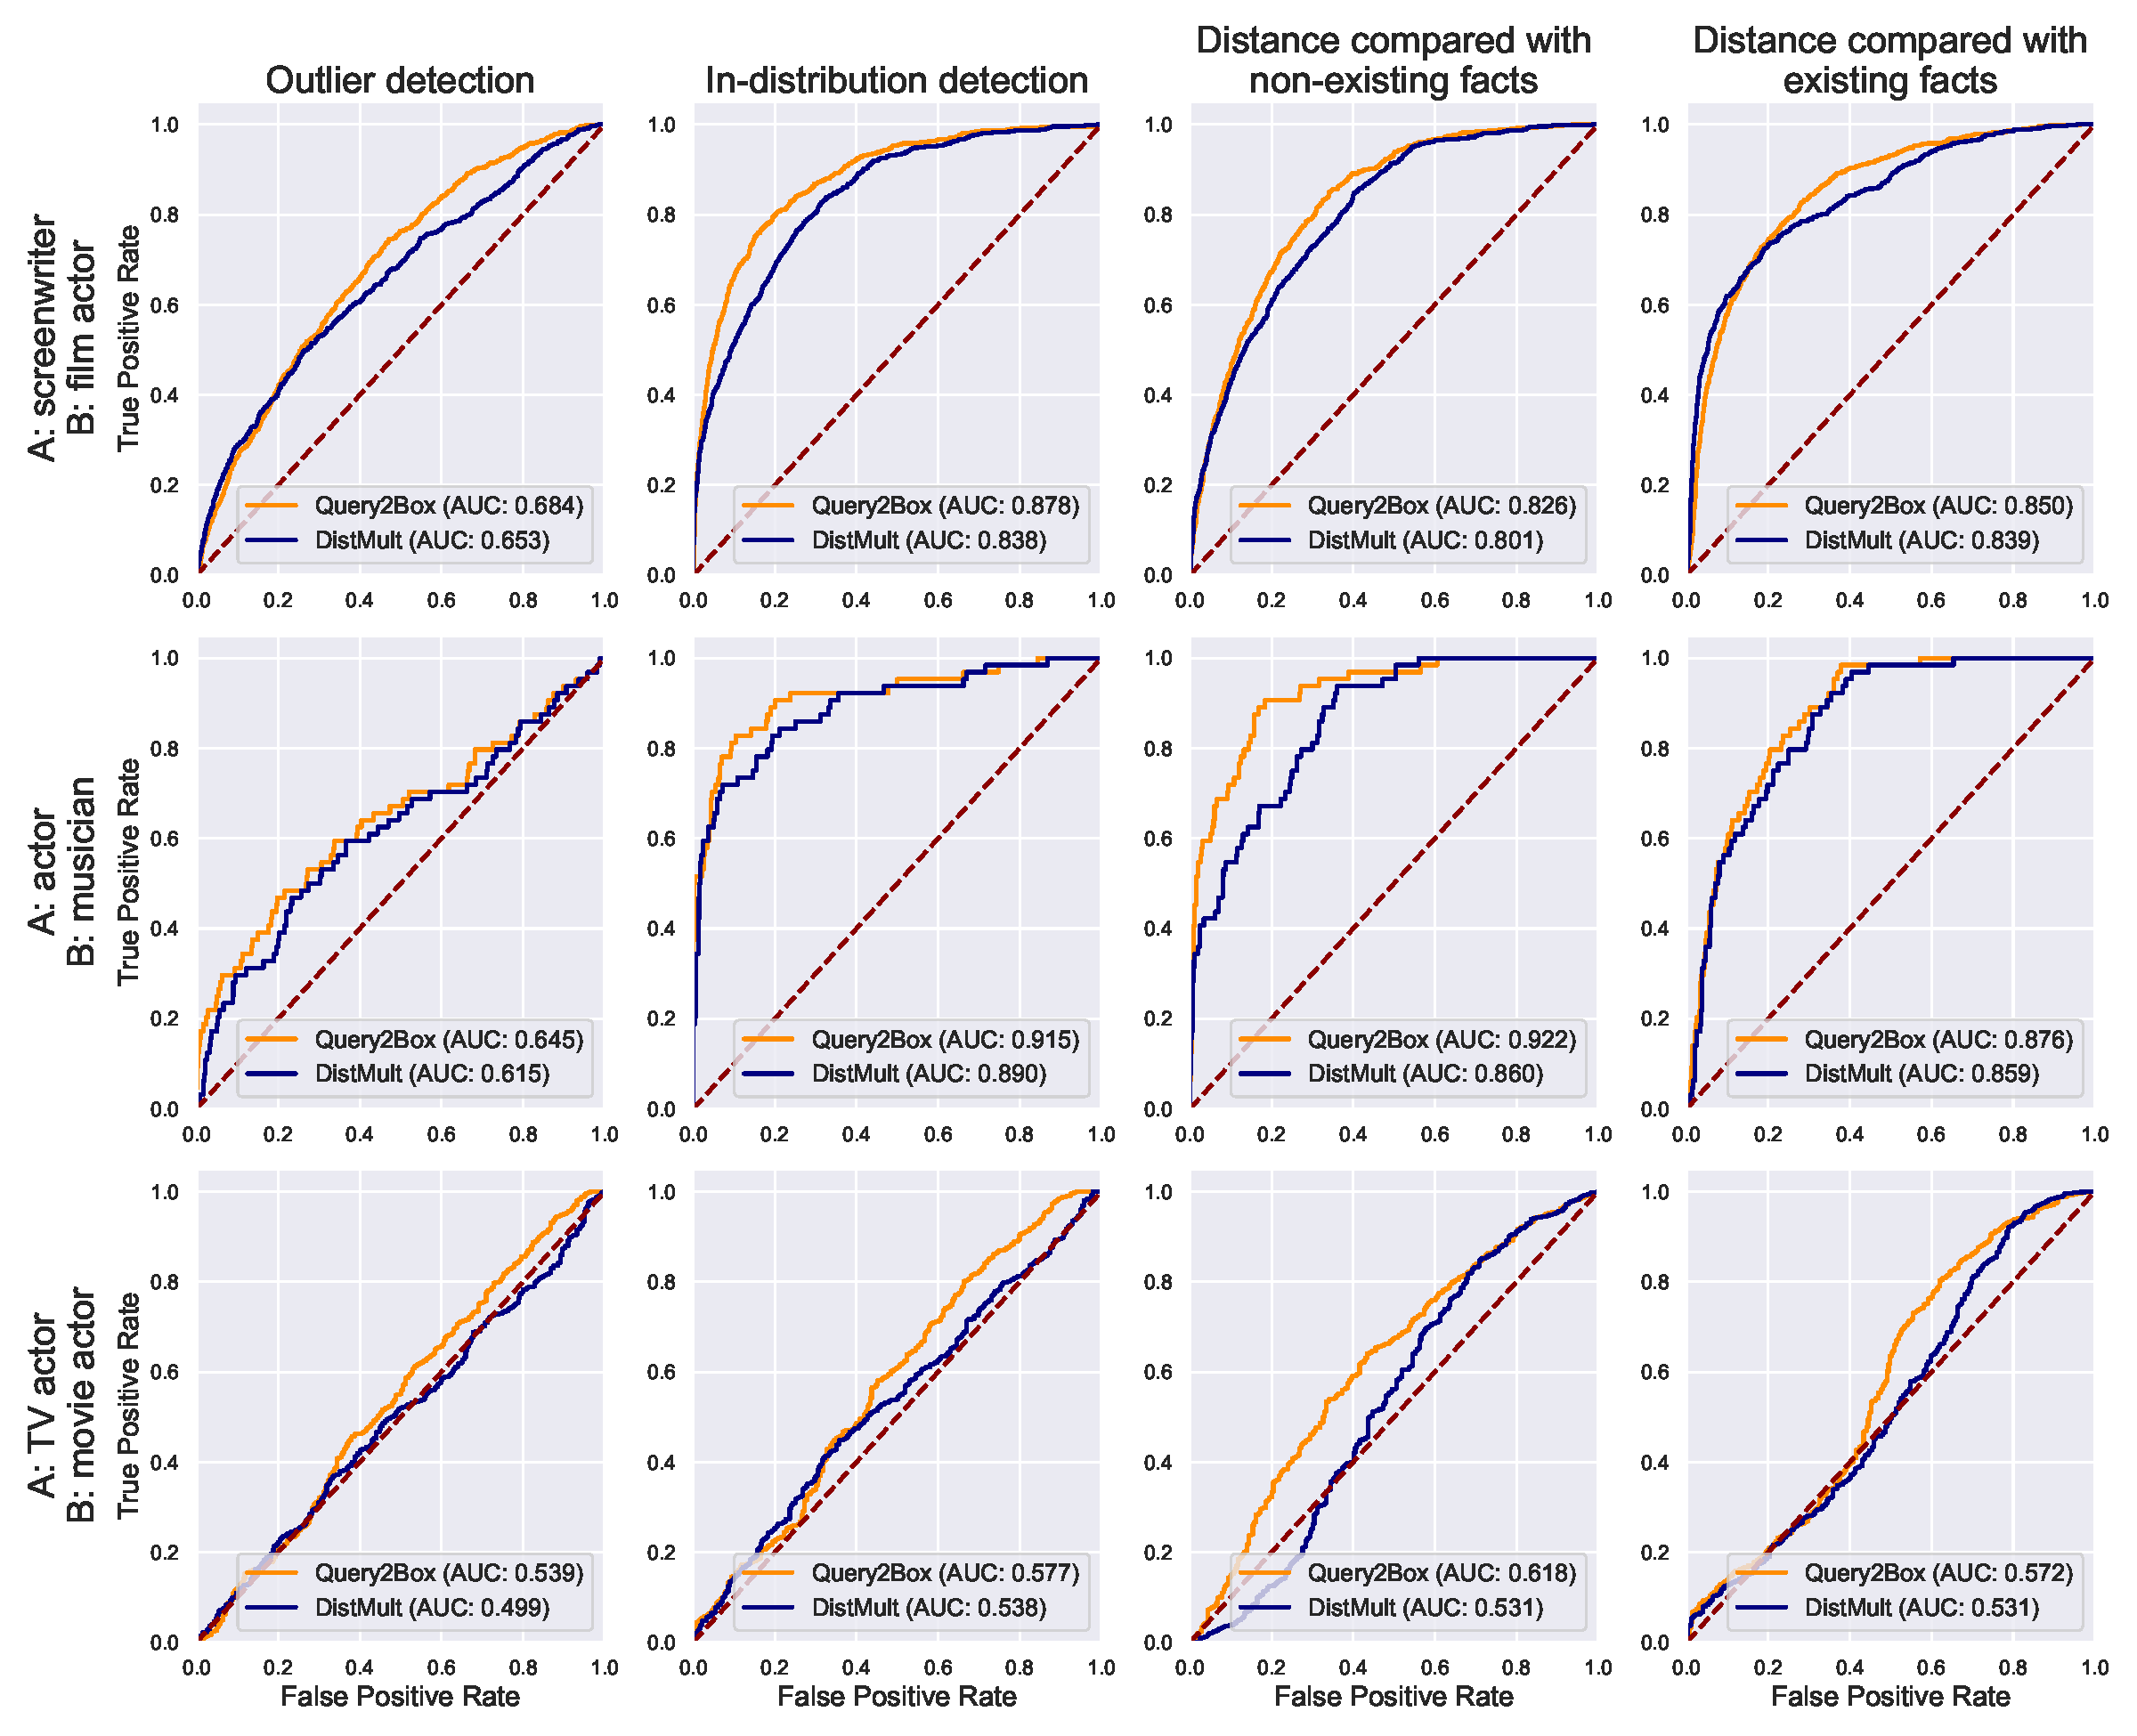
\includegraphics[width=1.7\columnwidth]{submissions/Ali2023/figures/final_roc.pdf}
      \caption{ROC-AUC curve of Query2box and DistMult in three case studies in fact verification. Query2box consistently achieves better performance than DistMult across cases and metrics. }
    \label{fig:roc-verification}
\end{figure*}
\end{comment}



\newparagraph{Stability}
We now measure the stability of different systems using the metrics we introduced in \Secref{sec:ali_method}.
We take all triples with \texttt{OccupationOf} as the relation type from the massive KG. Overall the dataset involves 6,566,224 queries of structure $(v_o, \texttt{OccupationOf}, ?)$ for which we measure the stability and consistency of rankings\iffalse across multiple runs (of training) for each method of interest\fi. 
Here we mainly consider two methods Query2box and DistMult, but not the MLMs due to their necessity of contexts for better ranking utility as discussed.
We train both models 5 times and measure the stability of both models using the metrics introduced in \Secref{sec:ali_consistency}.
As shown in Table \ref{tab:stability}, we find Query2box is more stable and consistent than DistMult since Query2box is trained on more complex multi-hop queries, which better captures the neighborhood structure for each fact.
\iffalse Specifically, for all the Kendall's Tau based methods (original, weighted or adaptive), Query2box is 0.474, 0.484, 0.432 better than DistMult.\fi For set-based overlap and rank-biased overlap, both methods achieve extremely high values. This is expected since the occupations of a celebrity are fixed across runs, and the overlap will always be 1 at the last step as we gradually compare the intersection of two sets starting from top-ranking items to the low-ranking ones.
Among evaluation metrics, our adaptive method can better characterize a more meaningful measurement of ranking stability than the vanilla Kendall's Tau and rank-biased overlap. As shown in Table \ref{tab:stability}, Query2box achieves higher performance in AdaptiveTau than the other two metrics. We argue such an adaptive metric is crucial in evaluating ranking stability in production. %Finally, we defer the experimental results for fact verification to \Secref{sec:ali_fact_ver_eval}.

\iffalse
\subsection{Performance  Improvements for Related Entity Search}
\revise{
We now present the performance improvements our hybrid query processing optimizations described in Section \ref{sec:ali_system}. We use a subset of KG entity embedding vectors, and compare the performance of our system against available existing hybrid query processing strategies (see \cite{mohoney2023high} for more details) using a randomly sampled and aggregated query workload from anonymized, historical queries. As shown in Table \ref{tab:end_to_end}, \hybridindex provides orders of magnitude performance improvements over best performing baselines for the related entity search task.
}

\begin{table}[t]
\small
\centering
	\caption{Slowdown for related entity search compared to \hybridindex @ Recall $>= .8$}\label{tab:end_to_end}
	\begin{tabular}{| c | c | c | c | c |}
		\hline
		 & \hybridindex & PreFilter & PostFilter & Range \\
		\hline
		\hline
		Slowdown & $1\times$ & $31\times$ & $136\times$ & NA \\
        \hline
	\end{tabular}
\end{table}
\fi
%%%%%%%%%%%%%%%%%%%%%%%%%%%%%%%%%%%%%%%%%%%%%%%%%%%%%%%%%%%%%%%%%%%%%%%%%%%%%%%%%%%%%%%%%%%%%%%%%%%%%%%%%%%%%%
\iffalse


\begin{figure*}
        \centering
      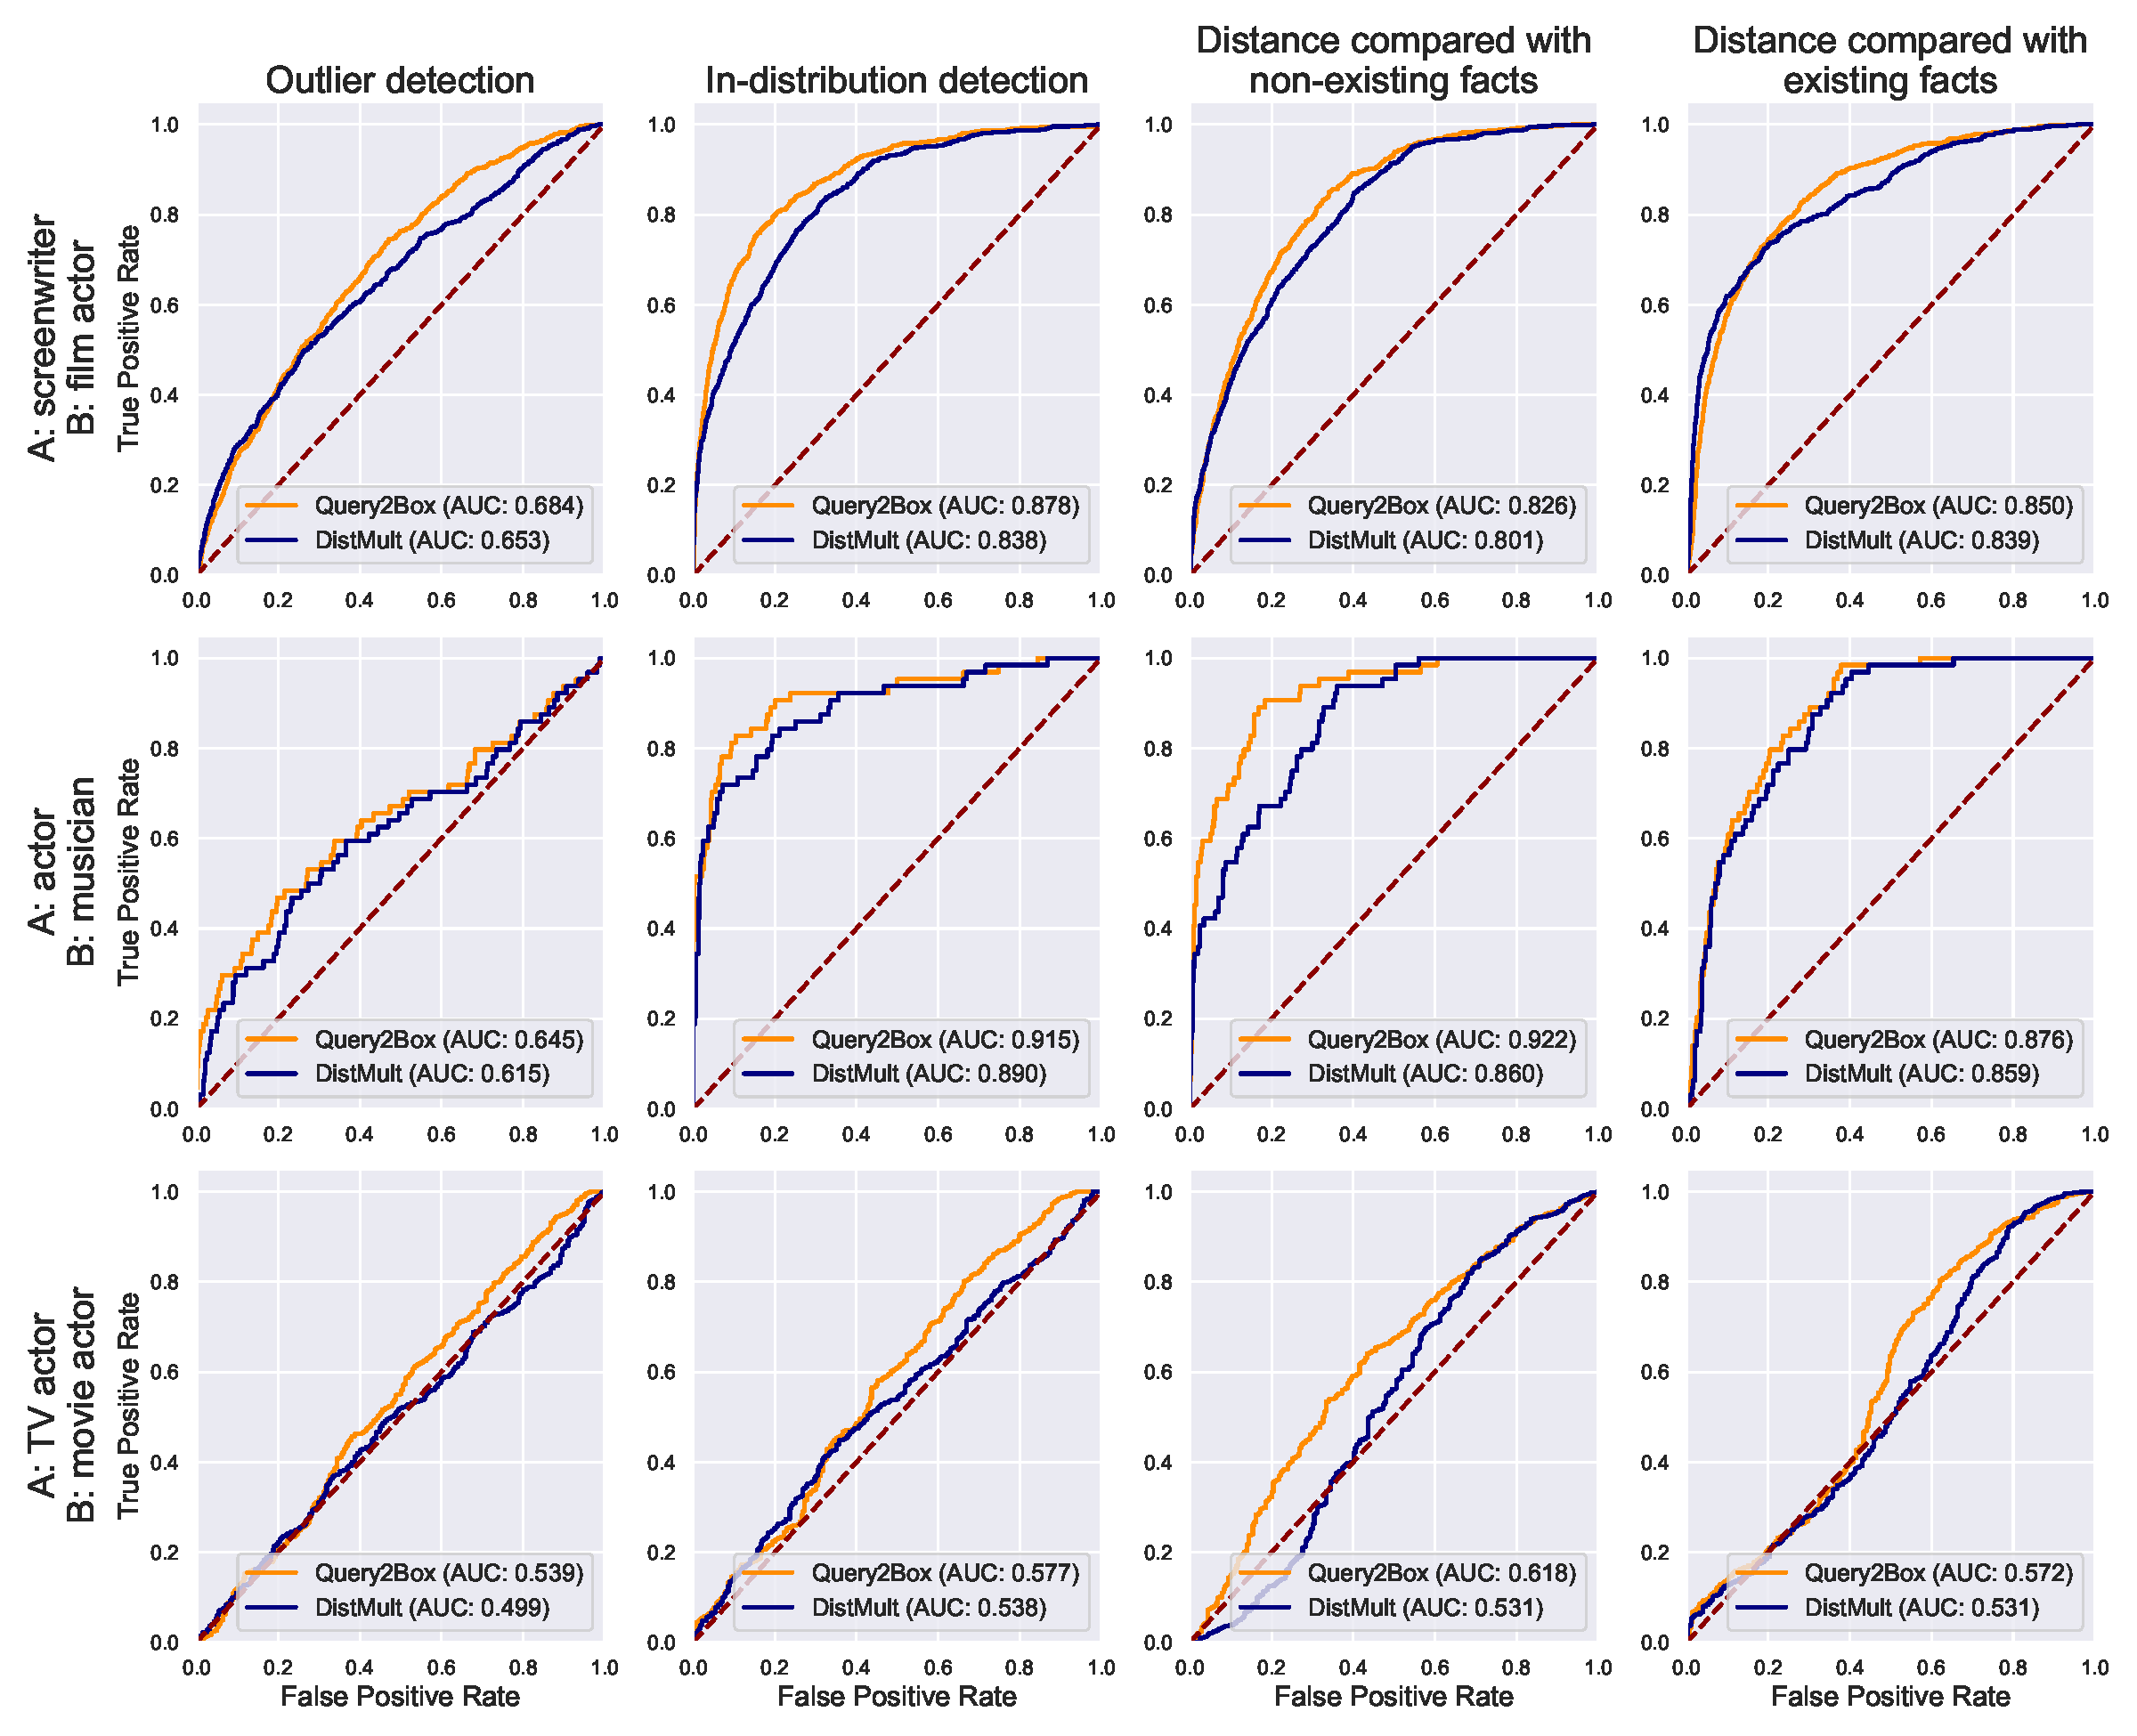
\includegraphics[width=1.5\columnwidth]{submissions/Ali2023/figures/final_roc.pdf}
      \caption{ROC-AUC curve of Query2box and DistMult in three case studies in fact verification. Query2box consistently achieves better performance than DistMult across cases and metrics. }
    \label{fig:roc-verification}
\end{figure*}


\section{Fact Verification Evaluation}\label{sec:ali_fact_ver_eval}
% Here we conduct experiments on the fact verification task. 
% Verifying the existing and missing facts on KG is one of the most important tasks in real-world production. Instead of giving a set of triplet facts directly for human curators to verify, we propose using our framework so that we can prioritize the promising facts for human curators to check first. 
We focus on queries about the occupation of a given celebrity with three case studies in fact verification task. In each case study, our system is given a set of celebrities $\{v_s\}$ of an occupation $A$, and the goal is to identify which celebrities among the set are likely to have occupation $B$. 
As introduced in \Secref{sec:ali_calibration}, we execute three different methods to calibrate the scores in our system. These methods include (1) outlier detection 
% -- we estimate a Gaussian distribution over sampled non-existing facts and verify whether a fact is an outlier to them using the Mahalanobis distance; 
(2) in-distribution sample detection 
% -- we sample existing facts related to the fact to verify and check whether the fact is an in-distribution sample; 
(3) distance compared with related facts.
% -- we calculate the score of a triplet fact (\ie, distance between the query and object as in \eqref{eq:lossfunc}, and also obtain the score of the sampled related facts, and compare to what extent the score of the fact is higher than that of the related facts. 
% For the method (3), we also use two definitions of related facts, including non-existing facts (same celebrity $v_s$ and relation {\tt OccupationOf} with an object entity $v_o$ where $(v_s, \texttt{OccupationOf}, v_o)$ does not exist on the graph) or existing facts (a set of $(v_s, \texttt{OccupationOf}, v_o)$ where $v_s$ is a semantically similar celebrity and the fact exists on the graph).


\newparagraph{Case study I -- A: screenwriter, B: film actor}
The first case study is that we aim to predict which celebrities in the given set of screenwriters are more likely to be also film actors. This case study is extremely challenging since screenwriters and film actors do not have a strong correlation, \ie, knowing a person is screenwriter does not give much information about whether this person is also a film actor. Together we have 5,715 screenwriters and we ask the human curators to first do a pass on each of the screenwriters and label whether they are also film actors. Finally we obtain a set of 715 screenwriters who are also film actors since they also appear in the IMDB database, while there are 5000 screenwriters who have never played in any movie so far. 
Then we further adopt the four different fact verification methods in order to classify whether the screenwriters are also film actors.
As shown in the first row in \Figref{fig:roc-verification}, we achieve an ROC-AUC of 0.878 and 0.838 for Query2box and DistMult respectively if we use the in-distribution detection formulation, \ie, whether \texttt{FilmActor} is considered as an in-distribution sample drawn from all the existing occupations of the specific celebrity. 
% Note the ROC-AUC would be 0.5 if we present all screenwriters directly to the human curators. 
Our framework demonstrates a significant boost in accuracy and especially the efficiency it brings to the verification process. If we consider the distance-based formulation, compared with the score of sampled related facts, Query2box achieves 0.826 when we sample non-existing facts as related facts, and 0.850 when we sample existing facts as related facts. 
% However, we find that outlier detection formulation is not as effective, with only 0.684 and 0.653 for Query2box and DistMult. For this case study, existing facts as related facts achieve a consistent better performance than non-existing facts.

\newparagraph{Case study II -- A: actor, B: musician}
The second case study is that given a set of actors, we aim to predict whether they are also musicians. This shares the similar situation with case study I, the two occupations -- \texttt{actor} and \texttt{musician} do not necessarily correlate with the other.
% Following the similar protocol as in the first case study, 
% We sample 564 actors and then pass them to human curators to check whether they are musicians or not. For each sample, we ask three human curators to check if each actor is a musician or not and then generate an answer based on the majority of votes. 
We collect a dataset of 64 actors with ``missing'' musician as their occupation and 500 actors who are truly not musicians so far. 
As shown in the second row in \Figref{fig:roc-verification}, all the four formulations achieve a ROC-AUC higher than 0.5. Specifically, with in-distribution detection formulation, we achieve 0.915 and 0.890 ROC-AUC score for Query2box and DistMult respectively. We may further improve the predictive performance of Query2box by using the distance-based verification. We push the performance to 0.922 for Query2box. Across all formulations, Query2box achieves consistently better performance than DistMult in prioritizing the promising facts. 

\newparagraph{Case study III -- A: TV actor, B: movie actor}
Finally, we check whether our proposed unified framework can predict whether TV actors are also movie actors. Unlike the previous two cases, \texttt{TVActor} and \texttt{MovieActor} are well correlated with each other. Most TV actors are also movie actors. Such a heuristic can be extremely predictive to solve this case study. 
% Given a set of TV actors but not movie actors, we can easily prioritize these TV actors and send them to human curators to verify whether they are also movie actors for most celebrities.
% However, even under such extreme circumstances, we would still aim to evaluate the performance of our proposed framework and validate whether it can achieve better performance than the heuristic when such heuristic may already work extremely well.
% Together we collect 5730 celebrities who are TV actors and send them to human curators to label whether they are also movie actors. 
% Due to the strong correlation between the two occupations, we find 5451 TV actors have also played roles in at least one movie.
Together we collect 5730 TV actors and among them 5451 have also played roles in movies.
We load the pretrained KG embeddings and calculate the score and residue of movie actor for each celebrity $v_o$ on query $(v_o, \texttt{OccupationOf}, \texttt{MovieActor})$.
Then we use the above four methods to classify whether we can use the score to classify those true missing movie actors from those who really have never appeared in any movie.
As shown in the last row in \Figref{fig:roc-verification}, compared with the results in the first two cases, here all our ROC-AUC scores of the four formulations are marginally over 0.5, where Query2box and DistMult achieves 0.577 and 0.525 ROC-AUC on average. 
% Although the heuristic is extremely effective in this case study, our framework still shows benefit over it. 
% Note that such strong heuristics do not often exist in most fact verification tasks. 
The results demonstrate that our framework can achieve comparable and even better performance than using strong heuristics, further validating the effectiveness of our unified solution.





% \newparagraph{Summary}
% Across the three case studies, Query2box achieves consistently better performance than the baseline DistMult, showcasing its effectiveness in prioritizing promising facts to human curators. Specifically, when there exists a nice heuristics to prioritize facts, Query2box achieves comparable or even better performance than using the heuristics. When no heuristics exist, KG embeddings demonstrate significant effectiveness than randomly assigning the facts for human curators to check.

\fi
\section{Use-case: Ranking for Related Entity Search}\label{sec:ali_related_entities}
%A key aspect of answering user queries in entity-centric experiences is to generate recommendation for other related entities that may be of interest within users' search contexts. For example, given the user query ``How tall is Taylor Swift'', we want to recommend a ranked list of top KG entities that are related to the query entity ``Taylor Swift'' and are aligned with users' search intent, \ie, find the most relevant KG entities that are ``Person'' and have a ``height'' attribute.

% Recommendation generation is a key aspect of answering user queries in entity-centric experiences, and finding related queries and other related entities for a given user query is critical entity-centric experience that can be powered by KGs. For example, given the user query ``How tall is Taylor Swift'', we want to construct queries of the form ``How tall is person?'' for other entities that uses can be interested given the query context. This requires us to find top KG entities that are related to ``Taylor Swift'' (i.e., ranking of KG entities based on their relatedness to the query entity) and align with users' intent (i.e., satisfying predicates in the query context such as their entity type is equal to ``Person'' and they have a non-NULL value for attribute ``height'') 
\revise{
Recommendation generation is a key component of question answering in entity-centric user experiences, and the task of providing a ranked list of KG entities related to that of users' query can be performed via fact ranking with KGE models.
}
Specifically, given a user query $q=(v_s, r, ?)$, the goal of related entity search is to find a ranking function $\rank{v_r}$ over a subset KG of entities $v_r \in \gR \subseteq \gV$ such that the query $q_r=(v_r, r, ?)$ is relevant to the original query, and $\rank{v_r}$ provides a ranking of each entity $v_r$ based on relatedness to the original query.  
% The task of finding ranked list of KG entities related to that of users' search context falls within the umbrella of recommendation generation.
We leverage the KGE models described in the previous sections 
% One can leverage the modern KGE techniques
for embedding a KG into a vector space and define \emph{relatedness} between two entities in a KG to be the similarity between their vector representations. Thus, we can use \emph{similarity search over KG embeddings} to find related entities for a given KG entity.
Depending on the specific application of related entity search, we can use different embedding models. As an example, if we are interested in relatedness in the ontology space of a KG, Poincaré embeddings \cite{poincare} is a suitable model. Otherwise, if we care about relatedness in the whole graph we can use either a shallow (\eg, DistMult \cite{distmult}) or reasoning-based embedding model. 

In addition to the use of KGE-based fact ranking for similarity based relatedness, the task of finding a ranked list of related KG entities for a query requires evaluating additional constraints for aligning answers with users' search intent. 
For instance, for the query ``How tall is LeBron James'', the goal is to find other ``Person'' entities that are \emph{related} to ``Lebron James'' and have the corresponding fact for the same predicate ``height''. 
Consequently,
related entity search use-case goes beyond the traditional vector similarity search and requires batch processing of \emph{hybrid queries}~\cite{mohoney2023high}. Hybrid queries are two part queries consisting of: (i) vector similarity search for retrieving the most similar entities in the embedding space; and (ii) evaluation of conjunction of relational constraints for ensuring the returned results are relevant to search context (\eg, only include ``Person'' entities). 
\revise{In addition to hybrid query processing, the task of related entity search exhibits following characteristics: (i) hybrid queries are evaluated in a \textbf{batch setting} over past user queries, (ii) and relational predicates in industrial KG workloads exhibit \emph{filter commonality} and \emph{filter stability}~\cite{sun2014fine}, allowing us to customize the system design based on \textbf{available prior workload} characteristics. 
% These characteristics necessitate new optimizations that are not covered by existing vector similarity search systems (see Section \ref{sec:ali_system}).
%Consequently, related entity search task imposes additional requirements for fact ranking with KGE models: 
% In addition to challenges of fact ranking over large-scale KG Performing batch inference for related entity search  has additional requirements due to the unique characteristics of the related entity search task: 
%(i) hybrid queries and their relational predicates require inference techniques beyond traditional vector similarity search-based solutions, and (ii) the volume and variety of candidate queries that are generated from available prior workloads render static, ``one size fits all'' solutions ineffective. 
To this end, we employ \hybridindex~\cite{mohoney2023high} hybrid vector similarity search system for  batch inference over KG embeddings and adopt the following suite of optimizations for \textit{high-throughput batch processing of hybrid queries}:
}

% The batch processing requirement of our workload is in fundamentally different from the existing industrial-scale systems focus on latency optimized online hybrid query processing. Therefore, in contrast to the other fact ranking tasks, our primary challenge here is performing \textit{high-throughput batch processing of hybrid queries} on KG embedding trained for the use-case. The requirements of related entity search use-case necessitate new optimizations that current vector database systems do not cover. To this end, we proposes the following suite of solutions including a \emph{workload-aware vector index} and a \emph{multi-query optimization technique}:

\textbf{Workload-aware vector index:}
% First, we introduce a new workload-aware index for vector databases.
Specialized vector indexes that either partition the data or form multi-level indexes over centroids are commonly used in vector databases to speed-up vector similarity search \cite{wang2021milvus}. \hybridindex utilizes the past workload information to guide the partitioning of the vectors in the underlying index in a  way that hybrid queries can be answered by accessing as few partitions as possible. By extending the concept of \emph{query-data routing trees (qd-trees)}~\cite{qd-tree} to vector databases, \hybridindex considers both vectors and relational predicates from a hybrid query workload when generating physical data layout at data loading time. The resulting data layout partitions the vectors using the distribution of the attributes associated with vectors, the attribute constraints, and similarity of vectors present in the hybrid query workload. We then use the resulting partitioning scheme to generate an index layout that enables processing a batch workload of hybrid queries by accessing vectors from as few partitions as possible.

\textbf{Batch query optimization:}
Second, we use \hybridindex's a multi-query optimization technique that (i) batches queries with similar attribute and vector similarity constraints; and (ii) performs batch vector distance computation against a posting list of vectors obtained from a clustering-based index over the vectors. 
This optimization is motivated by the fact that the set of candidate queries are computed from past user queries and evaluated in a batch setting, which enables computation sharing across queries.
% This optimization is motivated by the fact that our target hybrid query workloads need to be evaluated in a batch setting, enabling computation sharing across queries. 
Note that this optimization is orthogonal to the workload-aware vector index and is applicable to any clustering-based vector index.

We evaluate the performance improvements of these optimizations for related entity search over KG. We use a subset of KG entity embedding vectors, and we focus on ranking related entities for queries of the format \qu{What is the \texttt{[Predicate]} of \texttt{[Entity\_Name]}?}, similar to Section \ref{sec:ali_experiment}. Table \ref{tab:end_to_end} compares the performance of our solution against available existing hybrid query processing strategies (see \cite{mohoney2023high} for more details) using a randomly sampled and aggregated query workload from anonymized, historical queries. \hybridindex and its optimizations provide orders of magnitude performance improvements over best performing baselines for the related entity search task.
}

% \begin{table}[t]
% \small
% \centering
% 	\caption{Slowdown for related entity search compared to \hybridindex @ Recall $>= .8$}\label{tab:end_to_end}
% 	\begin{tabular}{| c | c | c | c | c |}
% 		\hline
% 		 & \hybridindex & PreFilter & PostFilter & Range \\
% 		\hline
% 		\hline
% 		Slowdown & $1\times$ & $31\times$ & $136\times$ & NA \\
%         \hline
% 	\end{tabular}
% \end{table}

\begin{table}[!t]
\small
\centering
	\caption{Slowdown for related entity search compared to \hybridindex @ Recall $>= .8$}\label{tab:end_to_end}
\begin{tabular}{lcccc}
                             & \textbf{HQI} & \textbf{PreFilter} & \textbf{PostFilter} & \textbf{Range} \\ \hline
\multicolumn{1}{c}{Slowdown} & 1$\times$    & 31$\times$         & 136$\times$         & NA            
\end{tabular}
\end{table}
% \section{Related Work}\label{sec:related_work}
\section{Conclusion}\label{sec:ali_conclusion}
In this work, we studied fact ranking over large-scale knowledge graphs. We evaluated to what extent modern knowledge graph embedding (KGE) models provide a solution for addressing the problem of fact ranking. We highlighted unique challenges associated with solving this task in industrial settings and evaluated different KGE and text-based embedding models. Our work demonstrated that, in contrast to neural language models or shallow KGE models, multi-hop reasoning models such as Query2Box can better meet user satisfaction.

% compared to  more stable than shallow KGE models with the latter not satisfying the stability properties required for stable fact ranking and fact verification services. We also showed that reasoning embedding models can be used to effectively prioritize facts to be verified by human graders. Finally, we evaluated the performance of modern generative natural language models on the tasks for fact ranking and verification and found that KG embedding models are competitive without requiring careful fine-tuning of the prompt that is used during inference.

\appendix
%\clearpage

\begin{thebibliography}{10}
\itemsep=1pt
\begin{small}


\bibitem{bollacker2008freebase} K.~Bollacker, C.~Evans, P.~Paritosh, T.~Sturge, and J.~Taylor. \newblock Freebase: a collaboratively created graph database for structuring human knowledge. \newblock {\em SIGMOD}, 2008.

\bibitem{transe} A.~Bordes, N.~Usunier, A.~Garcia-Dur\'{a}n, J.~Weston, and O.~Yakhnenko. \newblock Translating Embeddings for Modeling Multi-Relational Data. \newblock {\em Neural Information Processing Systems}, 2787–-2795, 2013.

\bibitem{bouraga2014knowledge} S.~Bouraga, I.~Jurerta, S.~Faulkner, and C.~Herssens. \newblock Knowledge-based recommendation systems: a survey. \newblock {\em International Journal of Intelligent Information Technologies}, 10(2):1--19, 2014.

% \bibitem{catherine2016personalized} R.~Catherine, and W.~Cohen. \newblock Personalized recommendations using knowledge graphs: A probabilistic logic programming approach. \newblock {\em ACM conference on recommender systems}, 325--332, 2016.

\bibitem{chami2020machine} I.~Chami, S.~Abu-El-Haija, B.~Perozzi, C.~Re, and K.~Murphy. \newblock Machine learning on graphs: A model and comprehensive taxonomy. \newblock {\em arXiv preprint}, arXiv:2005.03675, 2020.

\bibitem{DBLP:journals/corr/Cohen16b} W.~Cohen. \newblock TensorLog: {A} Differentiable Deductive Database. \newblock {\em arXiv preprint}, arXiv:1605.06523, 2016.

\bibitem{de2018formal} C.~De Sa, I.~Ilyas, B.~Kimelfeld, C.~R{\'e}, and T.~Rekatsinas. \newblock A formal framework for probabilistic unclean databases. \newblock {\em arXiv preprint}, arXiv:1801.06750, 2018.

\bibitem{knowledgevault} X.~Dong, E.~Gabrilovich, G.~Heitz, W.~Horn, N.~Lao, K.~Murphy, T.~Strohmann, S.~Sun, and W.~Zhang. \newblock Knowledge vault: A web-scale approach to probabilistic knowledge fusion. \newblock {\em ACM SIGKDD International Conference on Knowledge Discovery \& Data Mining}, 601--610, 2014.

\bibitem{Dong2019DataIA} D.~Xin, and T.~Rekatsinas. \newblock Data Integration and Machine Learning: A Natural Synergy. \newblock {\em ACM SIGKDD International Conference on Knowledge Discovery \& Data Mining}, 2019.

\bibitem{10.14778/2732951.2732962} X.~Dong, E.~Gabrilovich, G.~Heitz, W.~Horn, K.~Murphy, S.~Sun, and W.~Zhang. \newblock From Data Fusion to Knowledge Fusion. \newblock {\em VLDB}, 7(10):881--892, 2014.


% \bibitem{guo2022manu}, R.~Guo, X.~Luan, L.~Xiang, X.~Yan, X.~Yi, J.~Luo, Q.~Cheng, W.~Xu, J.~Luo, F.~Liu, and others. \newblock Manu: A Cloud Native Vector Database Management System. \newblock {\em arXiv preprint},  arXiv:2206.13843

\bibitem{hamilton2018embedding} W.~Hamilton, P.~Bajaj, M.~Zitnik, D.~Jurafsky, and J.~Leskovec. \newblock Embedding Logical Queries on Knowledge Graphs. \newblock {\em Neural Information Processing Systems}, 2018.

\bibitem{heidari2020record} A.~Heidari, G.~Michalopoulos, S.~Kushagra, I.~Ilyas, and T.~Rekatsinas. \newblock Record fusion: A learning approach. \newblock {\em arXiv preprint}, arXiv:2006.10208, 2020.

\bibitem{10.1145/3447548.3467342} H.~Huang, L.~Sun, B.~Du, C.~Liu, W.~Lv, and H.~Xiong. \newblock Representation Learning on Knowledge Graphs for Node Importance Estimation. \newblock {\em ACM SIGKDD Conference on Knowledge Discovery \& Data Mining}, 646-655, 2021.

\bibitem{apple_kp} I.~Ilyas, T.~Rekatsinas, V.~Konda, J.~Pound, X.~Qi, and M.~Soliman. \newblock Saga: A Platform for Continuous Construction and Serving of Knowledge At Scale. \newblock {\em ACM SIGMOD International Conference on Management of data}, 2022.

\bibitem{ilyas2019data} I.~Ilyas, and X.~Chu. \newblock Data Cleaning. \newblock {\em Morgan \& Claypool}, 2019.

\bibitem{ji2021survey} S.~Ji, S.~Pan, E.~Cambria, P.~Marttinen, and S.Y.~Philip. \newblock A survey on knowledge graphs: Representation, acquisition, and applications. \newblock {\em IEEE Transactions on Neural Networks and Learning Systems}, 2021.

\bibitem{kingma2014adam} D.~Kingma, and J.~Ba. \newblock Adam: A method for stochastic optimization. \newblock {\em International Conference on Learning Representations (ICLR)}, 2015.

\bibitem{lerer2019pytorch} A.~Lerer, L.~Wu, J.~Shen, T.~Lacroix, L.~Wehrstedt, A.~Bose, and A.~Peysakhovich. \newblock Pytorch-biggraph: A large-scale graph embedding system. \newblock {\em Conference on Machine Learning and Systems (MLSys)}, 2019.


\bibitem{liu2019roberta} Y.~Liu, M.~Ott, N.~Goyal, J.~Du, M.~Joshi, D.~Chen, O.~Levy, M.~Lewis, L.~Zettlemoyer, and V.~Stoyanov. \newblock Roberta: A robustly optimized bert pretraining approach. \newblock {\em arXiv preprint}, arXiv:1907.11692, 2019.

% \bibitem{mohoney2023high} J.~Mohoney, A.~Pacaci, S.~Chowdhury, A.~Mousavi, I.~Ilyas, U.F.~Minhas, J.~Pound, and T.~Rekatsinas. \newblock High-Throughput Vector Similarity Search in Knowledge Graphs. \newblock {\em arXiv preprint},  arXiv:2304.01926

\bibitem{mohoney2021marius} J.~Mohoney, R.~Waleffe, H.~Xu, T.~Rekatsinas, S.~Venkataraman. \newblock Marius: Learning Massive Graph Embeddings on a Single Machine. \newblock {\em USENIX Symposium on Operating Systems Design and Implementation (OSDI)}, 2021.


\bibitem{industry_kgs} N.~Noy, Y.~Gao, A.~Jain, A.~Narayanan, A.~Patterson, and J.~Taylor. \newblock Industry-Scale Knowledge Graphs: Lessons and Challenges. \newblock {\em Queue}, 17(2):48--75, 2019.


\bibitem{pujara2013knowledge} J.~Pujara, H.~Miao, L.~Getoor, and W.~Cohen. \newblock Knowledge graph identification. \newblock {\em International semantic web conference}, 542-557, 2013.


\bibitem{holoclean} T.~Rekatsinas, X.~Chu, I.~Ilyas, and C.~R\'{e}. \newblock HoloClean: Holistic Data Repairs with Probabilistic Inference. \newblock {\em VLDB Endowment}, 10(11):1190--1201, 2017.

\bibitem{ren2021smore} H.~Ren, H.~Dai, B.~Dai, X.~Chen, D.~Zhou, J.~Leskovec, and D.~Schuurmans. \newblock SMORE: Knowledge Graph Completion and Multi-hop Reasoning in Massive Knowledge Graphs. \newblock {\em arXiv preprint}, arXiv:2110.14890, 2021.

\bibitem{ren2020query2box} H.~Ren, W.~Hu, and J.~Leskovec. \newblock Query2box: Reasoning over Knowledge Graphs in Vector Space using Box Embeddings. \newblock {\em International Conference on Learning Representations (ICLR)}, 2020.

\bibitem{ren2020beta} H.~Ren, and J.~Leskovec. \newblock Beta Embeddings for Multi-Hop Logical Reasoning in Knowledge Graphs. \newblock {\em Neural Information Processing Systems (NeurIPS)}, 2020.

\bibitem{rossi2021knowledge} A.~Rossi, D.~Barbosa, D.~Firmani, A.~Matinata, P.~Merialdo. \newblock Knowledge graph embedding for link prediction: A comparative analysis. \newblock {\em ACM Transactions on Knowledge Discovery from Data}, 15(2)1--49, 2021.

\bibitem{sun2019rotate} Z.~Sun, Z.~Deng, J.~Nie, and J.~Tang. \newblock Rotate: Knowledge graph embedding by relational rotation in complex space. \newblock {\em International Conference on Learning Representations (ICLR)}, 2019.

\bibitem{sun2014fine} L.~Sun, M.J.~Franklin, S.~Krishnan, and R.S.~Xin. \newblock Fine-grained partitioning for aggressive data skipping, \newblock {\em ACM SIGMOD International Conference on Management of Data}, 1115-1126, 2014

\bibitem{sun2019re} Z.~Sun, S.~Vashishth, S.~Sanyal, P.~Talukdar, and Y.~Yang. \newblock A re-evaluation of knowledge graph completion methods. \newblock {\em arXiv preprint}, arXiv:1911.03903, 2019.

\bibitem{DBLP:conf/iclr/TabacofC20} P.~Tabacof and L.~Costabello. \newblock Probability Calibration for Knowledge Graph Embedding Models. \newblock {\em International Conference on Learning Representations (ICLR)}, 2020.

\bibitem{trouillon2016complex} T.~Trouillon, J.~Welbl, S.~Riedel, E.~Gaussier, G.~Bouchard. \newblock Complex embeddings for simple link prediction. \newblock {\em International Conference on Machine Learning (ICML)}, 2016.

% \bibitem{vartak2013chic} M.~Vartak, S.~Madden. \newblock CHIC: a combination-based recommendation system. \newblock {\em ACM SIGMOD International Conference on Management of Data}, 981--984, 2013.

\bibitem{wikidata} D.~Vrande\v{c}i\'{c}, and M.~Kr\"{o}tzsch. \newblock Wikidata: A Free Collaborative Knowledgebase. \newblock {\em Communications of the ACM}, 57(10):78--85, 2014.

 \bibitem{wang2021milvus} J.~Wang, X.~Yi, R.~Guo, H.~Jin, P.~Xu, S.~Li, X.~Wang, X.~Guo, C.~Li, X.~Xu, and others. \newblock Milvus: A purpose-built vector data management system. \newblock {\em ACM SIGMOD International Conference on Management of Data}, 2614--2627, 2021.

\bibitem{wei2021why} C.~Wei, S.M.~Xie, and T.~Ma. \newblock Why Do Pretrained Language Models Help in Downstream Tasks? An Analysis of Head and Prompt Tuning. \newblock {\em Advances in Neural Information Processing Systems}, 2021.

\bibitem{weikum2021knowledge} G.~Weikum. \newblock Knowledge graphs 2021: a data odyssey. \newblock {\em VLDB Endowment}, 14(12):3233--3238, 2021.

\bibitem{qd-tree} Z.~Yang, B.~Chandramouli, C.~Wang, J.~Gehrke, Y.~Li, U.F.~Minhas, P.~Larson, D.~Kossman, and R.~Acharya. \newblock Qd-Tree: Learning Data Layouts for Big Data Analytics. \newblock {\em ACM SIGMOD International Conference on Management of Data}, 193--208, 2020.

% \bibitem{yang2020pase} W.~Yang, T.~Li, G.~Fang, and H.~Wei. \newblock Pase: Postgresql ultra-high-dimensional approximate nearest neighbor search extension. \newblock {\em ACM SIGMOD International Conference on Management of Data}, 2241--2253, 2020.

\bibitem{distmult} B.~Yang, W.~Yih, X.~He, J.~Gao, L.~Deng. \newblock Embedding Entities and Relations for Learning and Inference in Knowledge Bases. \newblock {\em International Conference on Learning Representations (ICLR)}, 2015.

\bibitem{you2020handling} J.~You, X.~Ma, Y.~Ding, M.~Kochenderfer, and J.~Leskovec. \newblock Handling missing data with graph representation learning. \newblock {\em Advances in Neural Information Processing Systems (NeurIPS)}, 2020.

\bibitem{zhang2019quaternion} S.~Zhang, Y.~Tay, L.~Yao, Q.~Liu. \newblock Quaternion knowledge graph embeddings. \newblock {\em Advances in Neural Information Processing Systems (NeurIPS)}, 2019.

\bibitem{zhu2019graphvite} Z.~Zhu, S.~Xu, J.~Tang, and M.~Qu. \newblock Graphvite: A high-performance cpu-gpu hybrid system for node embedding. \newblock {\em The World Wide Web Conference (WWW)}, 2019.

\bibitem{poincare} M.~Nickel, and D.~Kiela. \newblock Poincaré embeddings for learning hierarchical representations \newblock {\em Advances in neural information processing systems (NeurIPS)}, 2017.

\bibitem{mohoney2023high} J.~Mohoney, A.~Pacaci, S.R.~Chowdhury, A.~Mousavi, I.~Ilyas, U.F.~Minhas, J.~POund, T.~Rekatsinas \newblock High-Throughput Vector Similarity Search in Knowledge Graphs \newblock{\em ACM SIGMOD/PODS International Conference on Management of Data (SIGMOD)}, 2023.

\end{small}
\end{thebibliography}


\end{document}